\documentclass[../main.tex]{subfiles}
\begin{document}
\clearpage
\setcounter{section}{0}% Сбрасываем счетчик в 0 (чтобы первое приложение было A)
\renewcommand{\thesection}{\Alph{section}}% Формат метки
\refstepcounter{section}
\section*{Приложение \Alph{section}.  Численный метод построения множеств достижимости при интегрально-квадратичных ограничениях на управление}% Заголовок с "Приложение A"
\label{app:A}% Метка с буквой (например, app:A)
\addcontentsline{toc}{section}{Приложение \Alph{section}. Численный метод построения множеств достижимости при интегрально-квадратичных ограничениях на управление}% Добавляем в оглавление
\renewcommand{\theequation}{\Alph{section}.\arabic{equation}}% Формат A.1 для формул
\setcounter{equation}{0}
В этом приложении приведен численный метод построения множеств достижимости нелинейных управляемых систем при интегрально-квадратичных ограничениях на управление, который был использован для расчета примеров в основном тексте диссертации.

Существуют различные методы приближенного построения множеств достижимости (пиксельные методы; методы, основанные на принципе максимума Понтрягина; методы, использующие эллипсоидальные и полиэдральные оценки).
Рассматриваемый метод относится к группе методов, которые можно назвать аналогами метода Монте-Карло. 
 
Отметим работы \cite{Gornov2015, Gornov2017}, ориентированные на геометрические ограничения на управление и развивающие методы, основанные на заполнении множества достижимости случайным набором точек, а также работы \cite{Lew2020, Lew2022}, в которых используется случайный выбор управлений и обеспечивается асимптотическая сходимость к выпуклой оболочке истинных множеств достижимости.
Используемый в диссертации подход основывается на случайном переборе управлений, разложенных по системе ортонормированных функций.

Повторим здесь постановку задачи и некоторые определения из Главы \ref{s1}.
На интервале времени $ t_0 \leqslant t \leqslant {T} $ рассмотрим нелинейную систему, аффинную по управлению
\begin{gather}\label{a1:common_nonlinear}
	\begin{gathered}
		\dot{x}(t)=f\big(t, x(t), u(t)\big), \qquad x(t_0) = x_0.
	\end{gathered}
\end{gather}

Здесь $ x \in \mathbb{R}^n $ ~--- вектор состояния, $ u \in \mathbb{R}^r $~--- управление, $t_0$, $ {T} $ ~--- некоторые фиксированные положительные числа.

Функция $ f: [t_0, {T}] \times \mathbb{R}^n \times \mathbb{R}^r \rightarrow \mathbb{R}^{n} $ предполагается непрерывной по $(t,x,u)$ и обладающей непрерывными производными по $ x $ на $ [t_0, {T}] \times \Omega \times \mathbb{R}^r $, где $\Omega$~--- некоторая область, $\Omega \subset \mathbb{R}^n$.

Всюду далее будем считать, что $x_0$ фиксирован и $x_0 \in \Omega $.
Также будем предполагать, что существует такое $\overline{\mu} > 0 $, что все решения (траектории) $ x(t, u(\cdot)) $ системы \eqref{a1:common_nonlinear}, отвечающие управлениям $u(\cdot) \in B_{\mathbb{L}_2[t_0, {T}]}(0,\overline{\mu})$, определены на интервале $ [t_0,{T}] $ и лежат в некотором выпуклом компакте $D \subset \Omega \subset \mathbb{R}^n$. 
 
Через $\mathbb{L}_2[t_0, {T}]$ здесь обозначено пространство интегрируемых с квадратом функций на интервале $[t_0, {T}]$. 
Под шаром $B_X(a,r)$ понимается замкнутый шар радиуса $r>0$ с центром в точке $a$ в линейном пространстве $X$ с нормой $\|\cdot\|_X$, $B_X(a, r) = \{x\in X: \|x-a\|_X \leqslant r \}$.
 
В дальнейшем, управление $ u(\cdot) $ будем выбирать из шара $ B_{\mathbb{L}_2[t_0, {T}]}(0,\mu) $, где $ 0 < \mu < \overline{\mu} $, т.\,е.
\begin{gather}\label{a1:constraints}
	\int\limits_{t_0}^T u^{\top}(t) u(t) \ dt \leqslant \mu^2.
\end{gather}
 
{\sl Множеством достижимости } $ G(T,\mu) $ системы \eqref{a1:common_nonlinear} в пространстве состояний в момент времени $ T $ назовем множество всех концов траекторий $ x(T, u(\cdot)) \in \mathbb{R}^n $, которые могут быть порождены управлениями $ u(\cdot) \in B_{\mathbb{L}_2}(0,\mu) =\left\lbrace u:\lVert u(\cdot)\rVert^2_{\mathbb{L}_2} \leqslant \mu^2\right\rbrace $,
\begin{gather*}
	G(T,\mu)=\{x\in \mathbb{R}^n:\exists u(\cdot)\in B_{\mathbb{L}_2}(0,\mu),\; x=x(T,u(\cdot))\}.
\end{gather*}
 
Как и в других численных методах построения множеств достижимости, основанных на алгоритме Монте-Карло, идея обсуждаемого метода состоит в случайном переборе достаточно большого конечного набора управлений $u_i(\cdot) \in U \subset B_{\mathbb{L}_2[t_0, {T}]}(0,\mu) $, $ i = 1, \dots, N$, каждое из которых удовлетворяет ограничению \eqref{a1:constraints}.
Для каждого управления производится интегрирование системы \eqref{a1:common_nonlinear} и запоминается конечная точка полученной траектории $x_i(T, u_i(\cdot))$, $ i = 1, \dots, N$. 
По определению, все такие точки лежат в множестве достижимости $G(T,\mu)$.
 
Ключевым вопросом является конструирование множества управлений $U$.
 В случае геометрических ограничений, управления, которые ведут на границу, как правило, относятся к классу кусочно-постоянных (ступенчатых или релейных) функций.
 Соответственно, для того, чтобы точнее построить границу множества достижимости, разумно строить множество перебираемых управлений именно из таких функций. 
 В случае же интегральных квадратичных ограничений, систему можно перевести в любую точку множества достижимости (в том числе в граничную) используя только непрерывные управления, поэтому достаточно перебирать непрерывные функции. 
 Рассматриваемый метод предполагает заполнение этого множества управлениями вида 
 \begin{gather}\label{a1:control}
 	u_i(t) = C_i p (t),
 \end{gather}
 где $ i = 1, \dots, N$, $p(t) = \big(p_{0}(t),p_{1}(t),\dots,p_{k}(t)\big)$, $p: [t_0, {T}] \rightarrow \mathbb{R}^{k+1} $ --- вектор-функция, состоящая из ортонормированных скалярных функций в пространстве $\mathbb{L}_2[t_0, {T}]$, а $C_i \in \mathbb{R}^{r \times k+1}$ --- матрица коэффициентов. 
	 
 Например, $p(t)$ для интервала $[0,1]$ можно составить из полиномов Лежандра:
 \begin{gather*}
 	p_0(t) = 1, \quad p_1(t) = 3.46t-1.73, \quad p_2(t) = 13.41t^2 - 13.41t + 2.24, \\ \quad 
 	p_3(t) = 52.92t^3 - 79.37t^2+31.75t -2.65, ...
 \end{gather*}
 
 Ортонормированные полиномы позволяют легко учитывать интегральные квадратичные ограничения.
 Для того, чтобы такие управления $u_i(\cdot)$ удовлетворяли ограничению \eqref{a1:constraints} оказывается достаточно, чтобы $\|C_i\| \leqslant \mu$, где $\|\cdot\| $ --- фробениусова норма матрицы.
 Действительно,
 \begin{gather}\label{a1:norm1}
 	 u^{\top}(t) u(t) = \big(C p(t)\big)^{\top} \big(C p(t)\big) = p^{\top}(t) C^{\top} C p(t) = \sum_{i=0}^k \sum_{j=0}^k a_{ij} p_i(t) p_j(t),
 \end{gather}
 где $ A = \{a_{ij}\}_{1\leqslant i,j \leqslant k + 1} = C^{\top} C \in \mathbb{R}^{(k+1) × (k+1)} $.
 
 Подставляя выражение из \eqref{a1:norm1} в \eqref{a1:constraints}, получим
 \begin{gather}\label{a1:norm2}
 		\int\limits_{t_0}^T u^{\top}(t) u(t) \ dt = \sum_{i=0}^k \sum_{j=0}^k a_{ij} \int\limits_{t_0}^T p_i(t) p_j(t) dt.
 \end{gather}
 Из ортонормированности $p$ следует, что 
 \begin{gather}
 	\int\limits_{t_0}^T p_i(t) p_j(t) dt = \delta_{ij}. 
 \end{gather}
 Поэтому, все члены выражения справа в \eqref{a1:norm2} с $i \neq j$ равны нулю, и остается 
 \begin{gather}
 	\int\limits_{t_0}^T u^{\top}(t) u(t) \ dt = \sum_{i=0}^k a_{ii} = \operatorname{trace}(A) = \operatorname{trace}(C^{\top} C) = \| C\|^2.
 \end{gather}
 
 Таким образом, выбирая различные матрицы $C$, удовлетворяющие неравенству $\| C\| \leqslant \mu $ можно получать различные управления $u(t) = C p(t)$, удовлетворяющие ограничению \eqref{a1:constraints}.
 
 Заметим, что процедура случайного перебора таких матриц $C$ может быть организована различными способами, о некоторых из которых будет рассказано ниже.
 
 Описанный алгоритм построения множества достижимости системы \eqref{a1:common_nonlinear} с ограничениями \eqref{a1:constraints} легко реализовать, что видно из псевдокода \ref{ap:method}.
 \RestyleAlgo{ruled}
 \begin{algorithm}[hbt!]
 	\SetKwFunction{Propagate}{Propagate}
 	\SetKwInOut{Parameters}{Параметры}\SetKwInOut{Data}{Данные}\SetKwInOut{Output}{Выход}
 	\Parameters{количество точек $N$, степень полиномов $k$;}
 	\Data{ресурс управления $\mu$, начальное условие $x_0$, $t_0$, $T$;}
 	\Output{$\{x_i\}_{i = 1}^{N}$;}
 	$p(t) \gets $ ортонормированные полиномы в $\mathbb{L}_2[t,T]$\;
 	\For{$i\leftarrow 0$ \KwTo $N$}{
 		$C \gets $ случайная матрица, такая, что $ \|C\| \leqslant \mu $\;
 		$u(t) \gets C p(t)$\;
 		$x_i \gets $ проинтегрировать уравнение \eqref{ap:nonlinear_system1} с начальным условием $x_0$, управлением $u(t)$ на интервале $\big[t_0, T\big]$\; }
 	\caption{Численный метод построения множеств достижимости}
 	 \label{ap:method}
 \end{algorithm}
 
 Полученное с помощью такого алгоритма множество концов траекторий $\{x_i\}_{i = 1}^{N}$ при достаточно большом $N$ и $k$ дает представление о форме и размерах множества достижимости и его проекций. 
 Повышение точности при увеличении числа ортонормированных функций $k$ следует из теоремы о наилучшем приближении в гильбертовом пространстве (см., например, \cite{Kolmogorov}). 
 
 Фактически, представление \eqref{a1:control} можно считать частичной суммой ряда Фурье по системе функций $p(t)$ для некоторой функции из $\mathbb{L}_2[t_0, {T}]$. 
 Из равенства Бесселя следует, что ошибка аппроксимации уменьшается при увеличении количества членов ряда. 
 
 Таким образом, при увеличении $k$ увеличивается точность аппроксимации непрерывных управлений. 
 Однако, увеличение $k$ может приводить к накоплению ошибок округления при  формировании ортонормированной системы $p(t)$ с использованием алгоритма Грама-Шмидта (CGS, classical Gram–Schmidt). 
 От использования этого алгоритма можно отказаться при использовании полиномов Лежандра, для которых существуют рекуррентные формулы, обеспечивающие численную устойчивость. 
 Но при использовании произвольных базисных функций (например, гармонических или радиально-базисных функций) для сохранения точности при увеличении $k$ необходимо использовать более устойчивые алгоритмы ортогонализации, например, модифицированный алгоритм Грама-Шмидта (MGS, modified Gram-Schmidt).
 
 Итерации алгоритма независимы друг от друга, что позволяет вычислять концы траекторий $x_i$ параллельно. 
 Это, в свою очередь, позволяет увеличивать $N$, сохраняя время работы алгоритма в разумных пределах.
 
 В следующих подразделах будут приведены примеры использования этого алгоритма для расчета точек множества достижимости различных систем, и обсуждены некоторые эффекты, возникающие при его использовании.
 
 \subsection{Простые примеры}
 \begin{figure}[ht!] 
 	\hspace{-2.5ex}
 	\begin{minipage}[b]{.3\linewidth} 
 		\small
 		\centering 
 		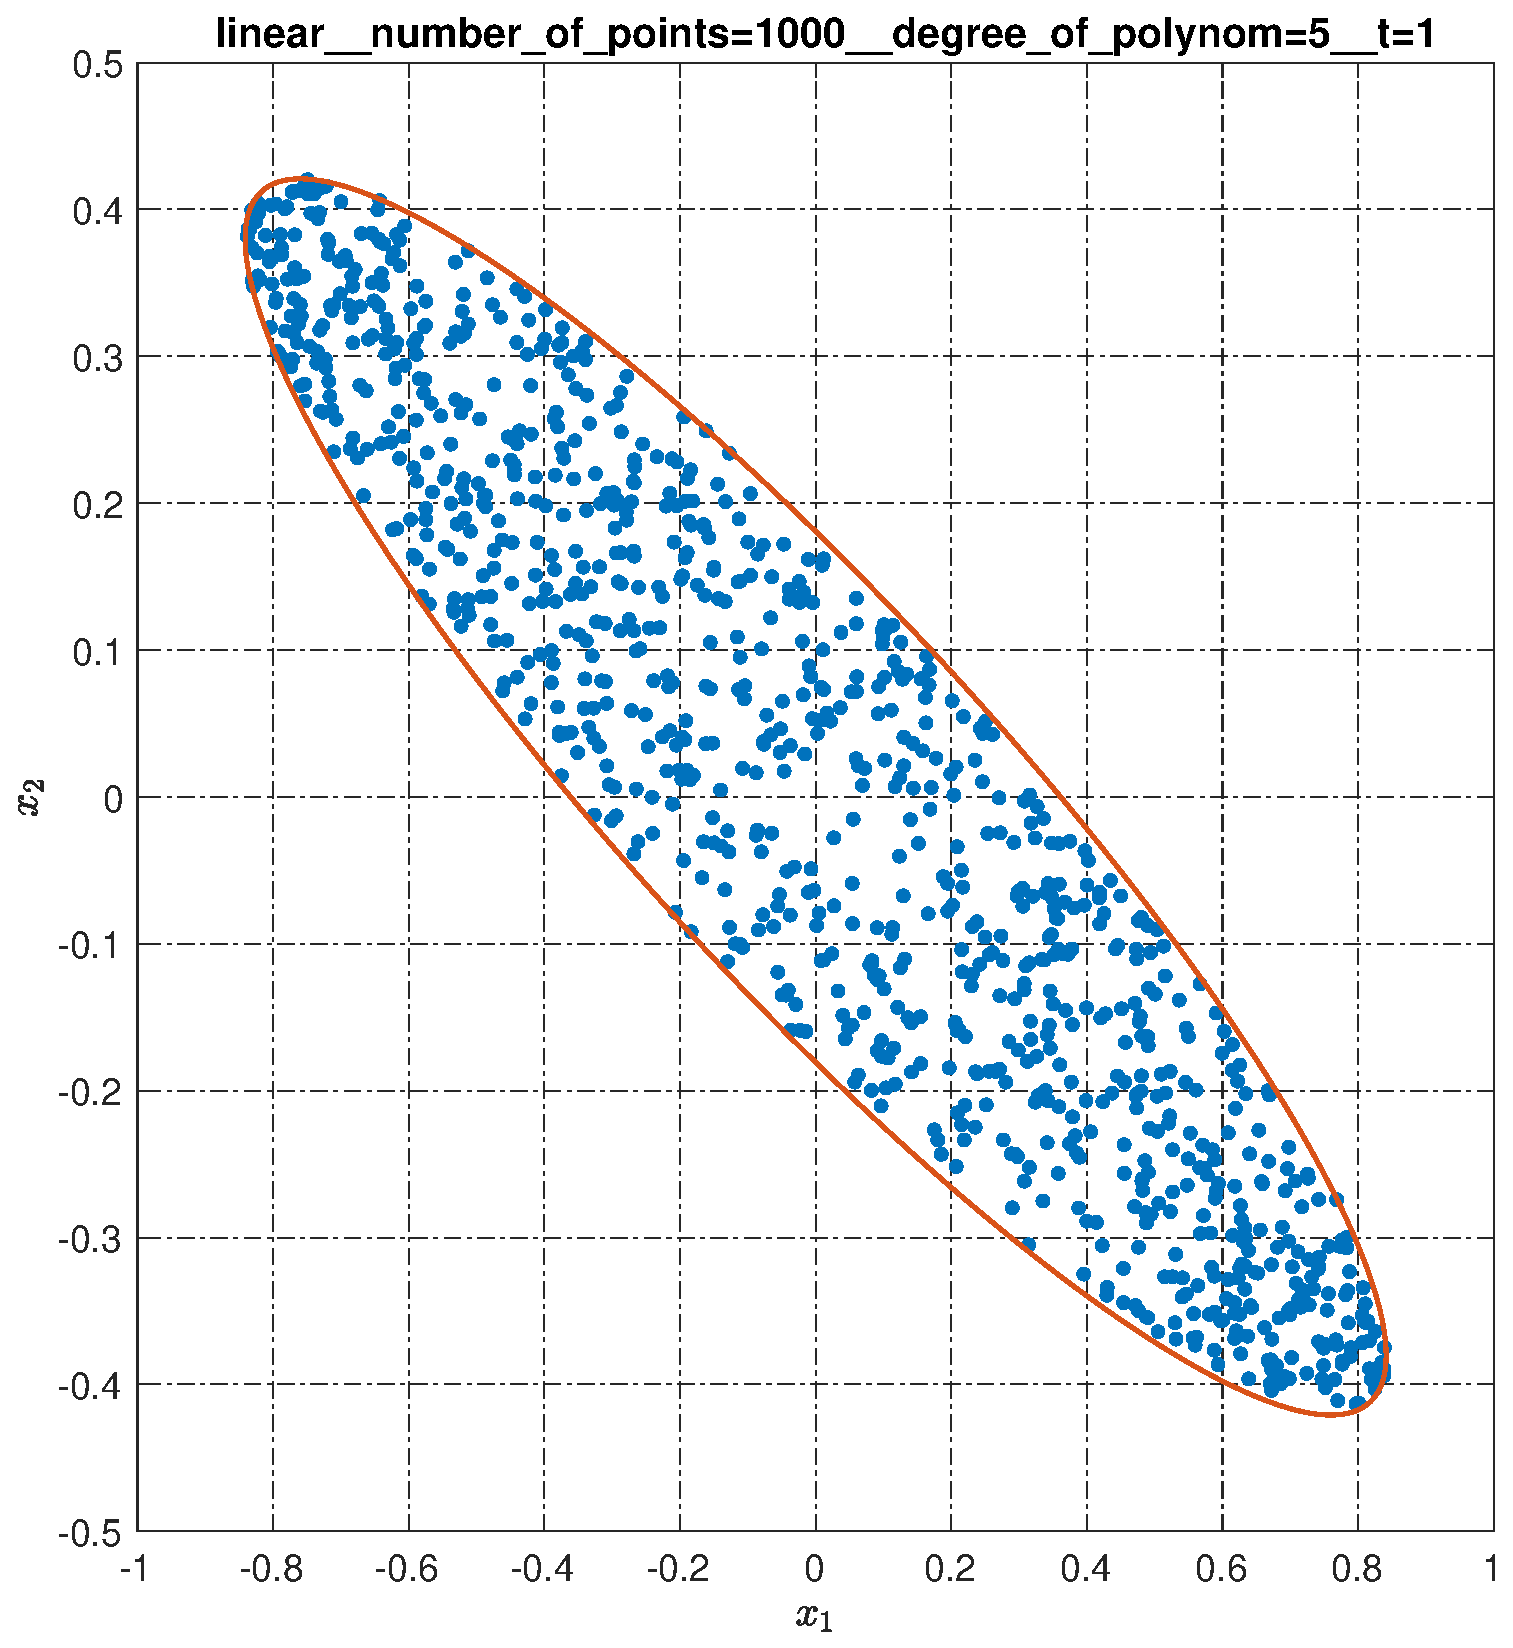
\includegraphics[width=\linewidth]{images/linear__number_of_points=1000__degree_of_polynom=5__t=1.eps}
 		\subcaption{$ N = 10^3 $, $ k = 5 $, $T = 1 $}
 		\label{fig:ap:linearN103k5T1} 
 	\end{minipage}
 	\hfill
 	\begin{minipage}[b]{.3\linewidth} 
 		\small
 		\centering
 		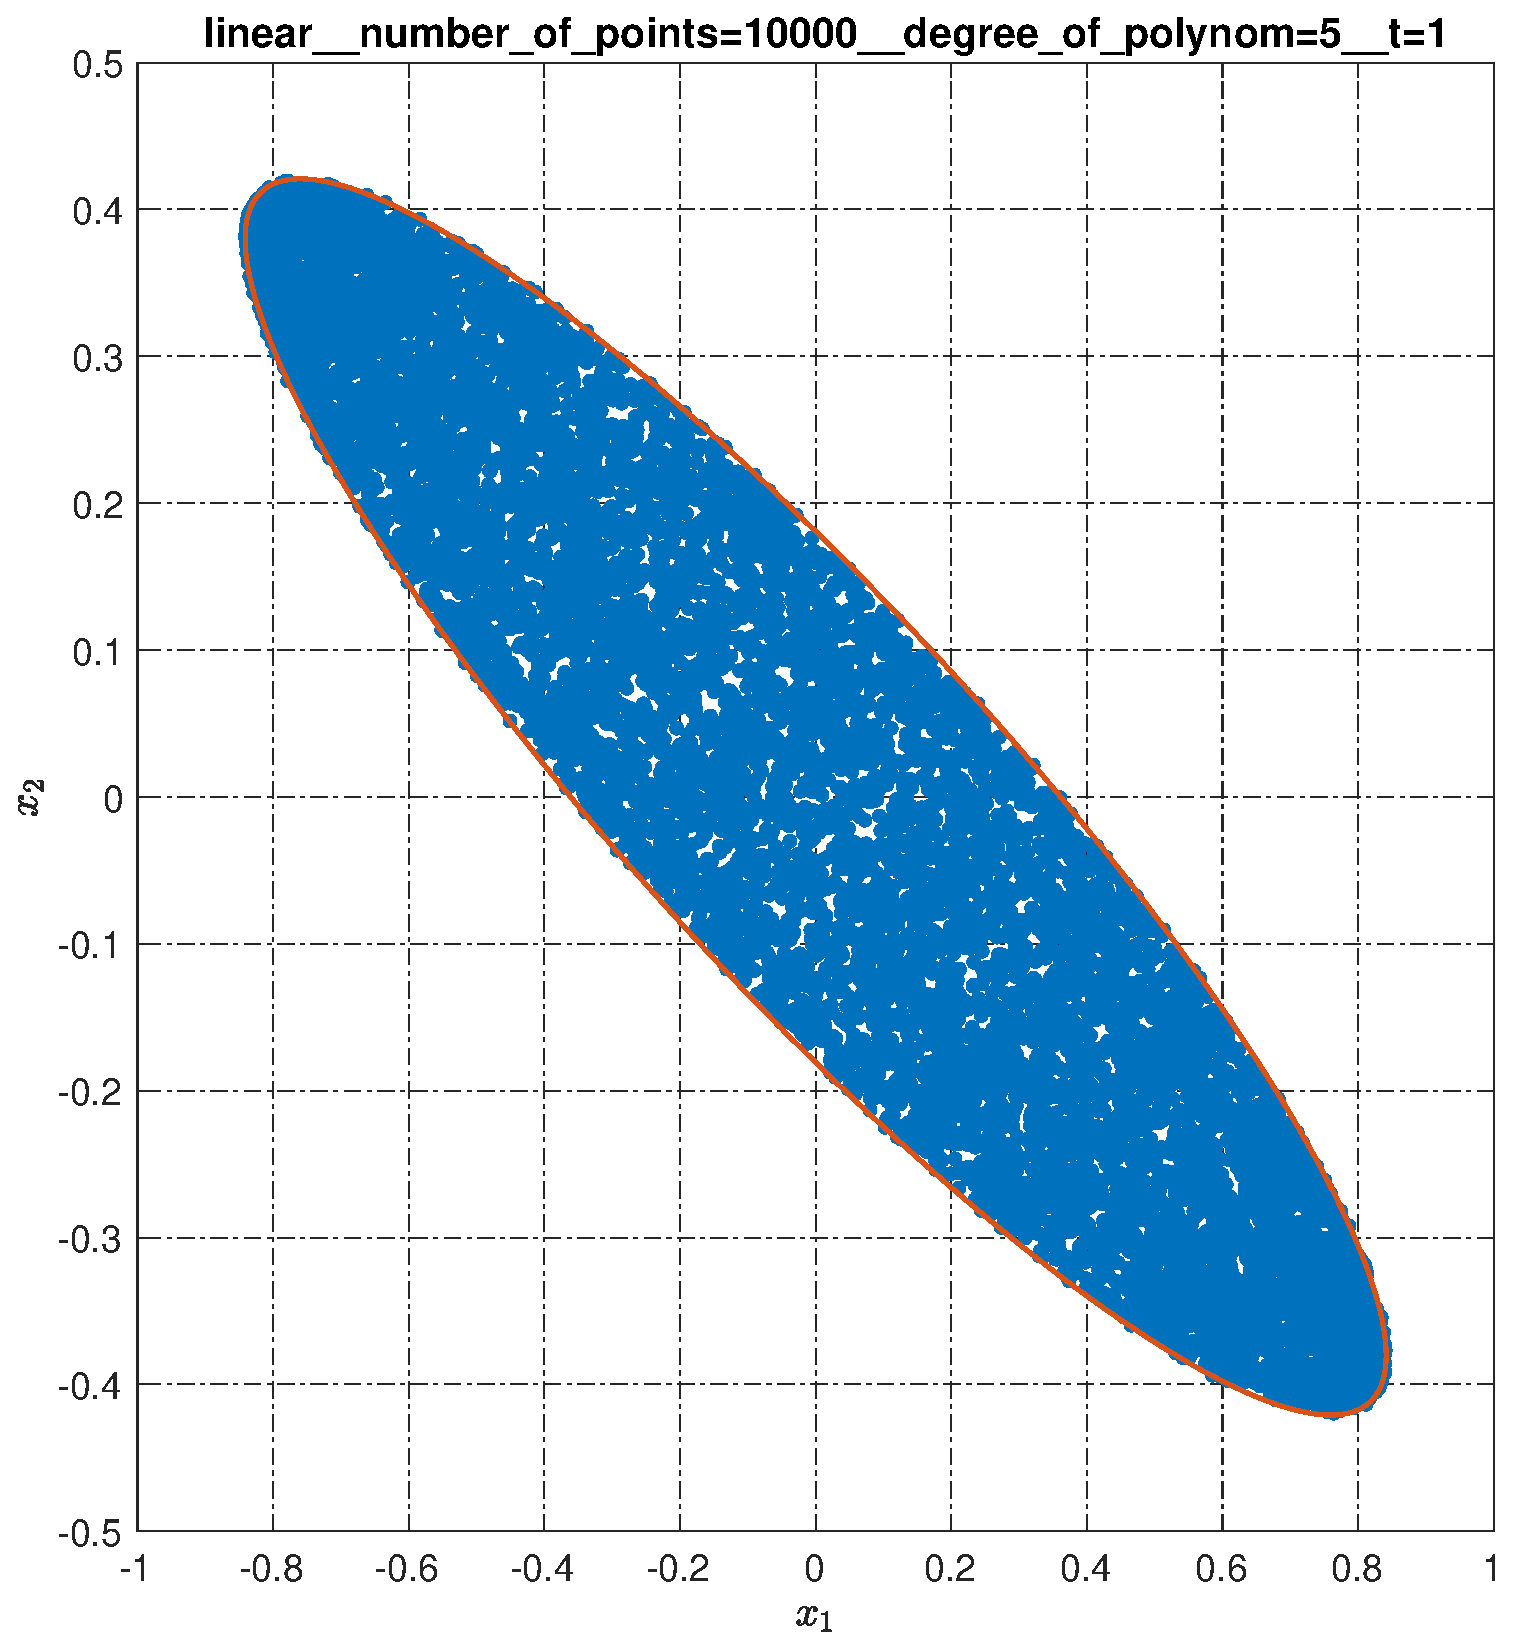
\includegraphics[width=\linewidth]{images/linear__number_of_points=10000__degree_of_polynom=5__t=1.eps}
 		\subcaption{$ N = 10^4 $, $ k = 5 $, $T = 1 $ }
 	\end{minipage} 
 	\hfill
 	\begin{minipage}[b]{.3\linewidth} 
 		\small
 		\centering
 		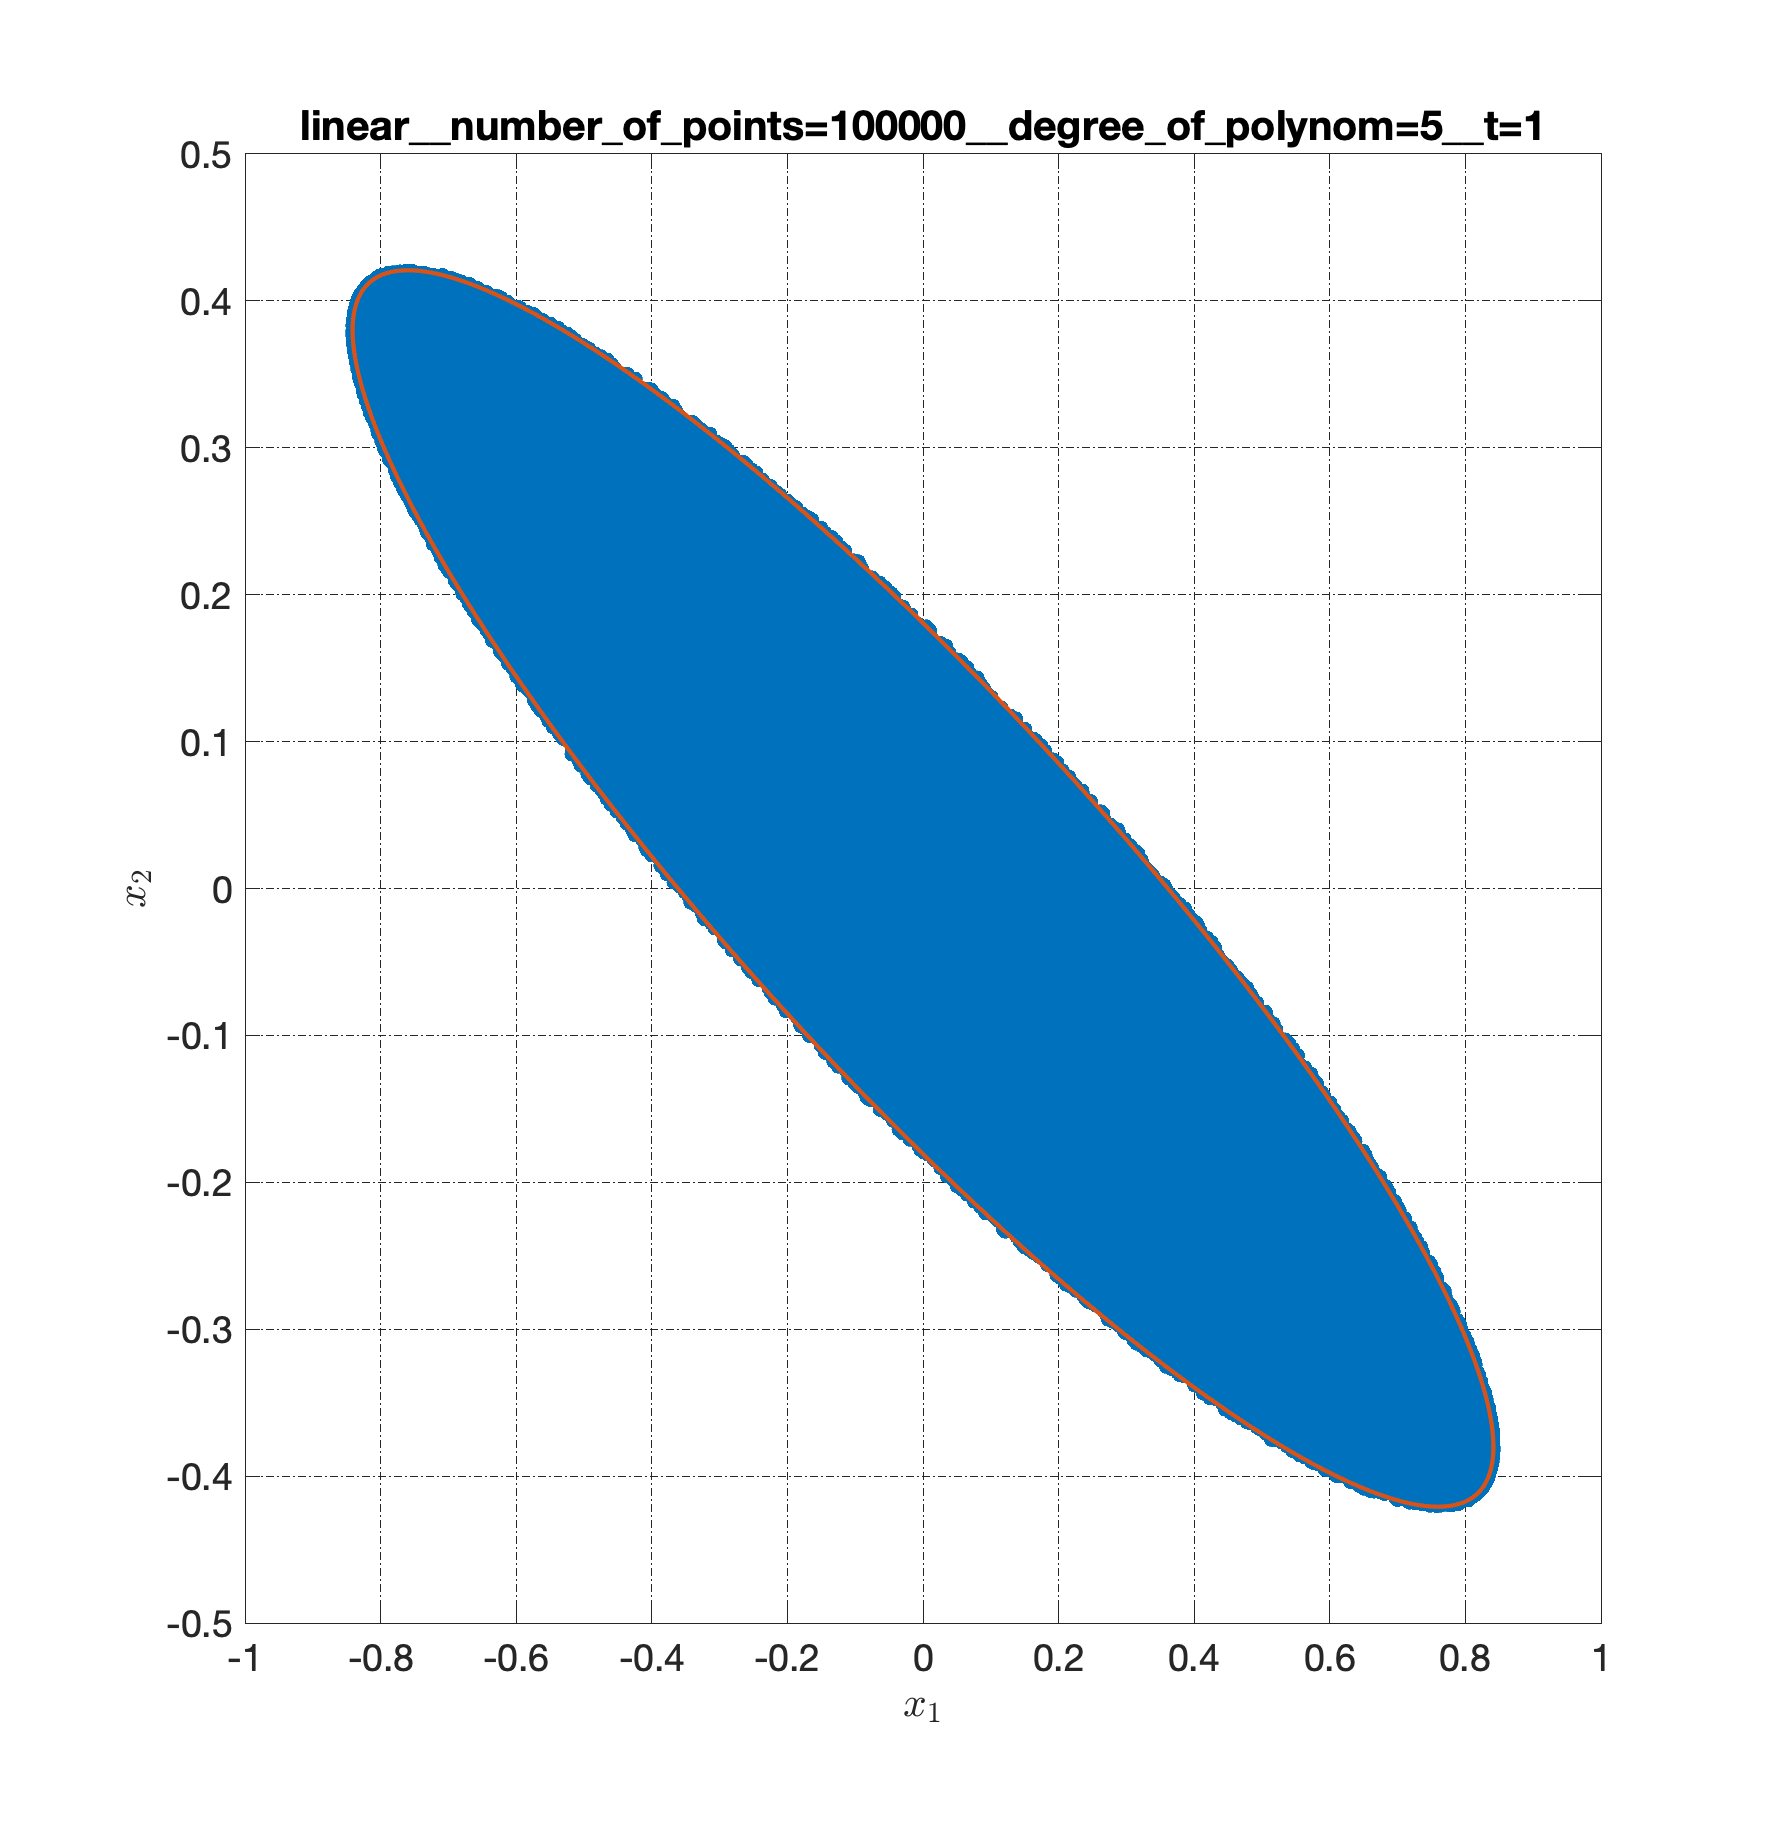
\includegraphics[width=\linewidth]{images/linear__number_of_points=100000__degree_of_polynom=5__t=1.eps}
 		\subcaption{$ N = 10^5 $, $ k = 5 $, $T = 1 $}
 	\end{minipage} 
 	\vfill
 	\begin{minipage}[b]{.3\linewidth} 
 		\small
 		\centering 
 		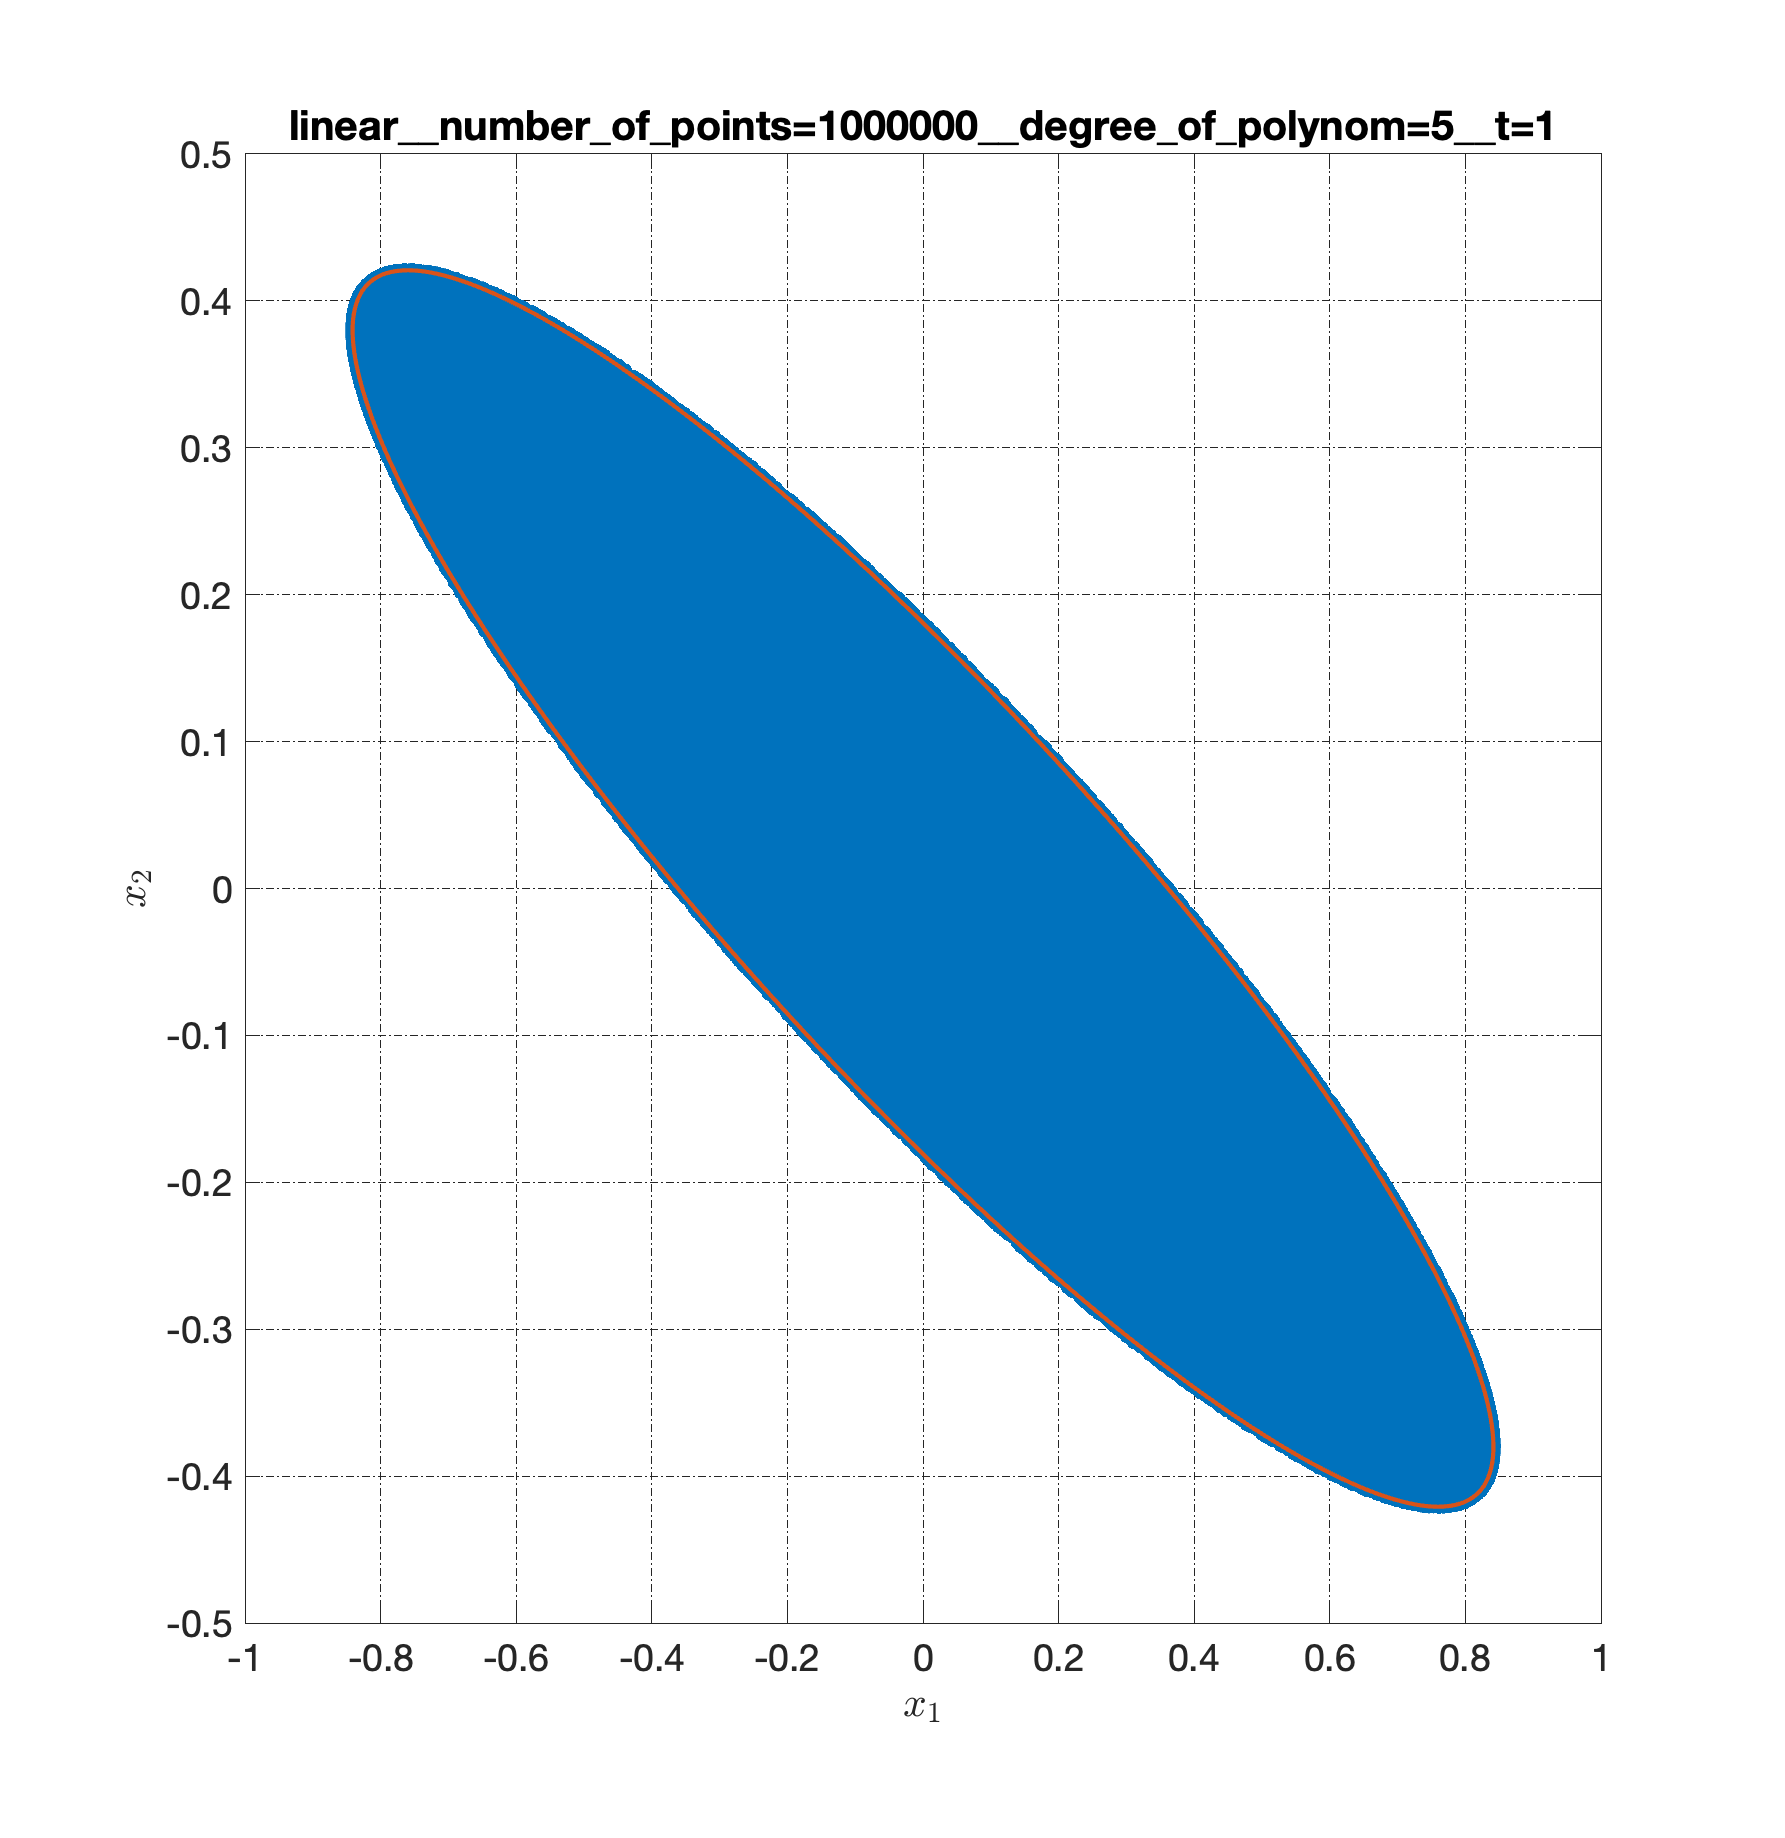
\includegraphics[width=\linewidth]{images/linear__number_of_points=1000000__degree_of_polynom=5__t=1.eps}
 		\subcaption{$ N = 10^6 $, $ k = 5 $, $T = 1 $}
 		\label{fig:ap:linearN106k5T1}
 	\end{minipage}
 	\hfill
 	\begin{minipage}[b]{.3\linewidth} 
 		\small
 		\centering
 		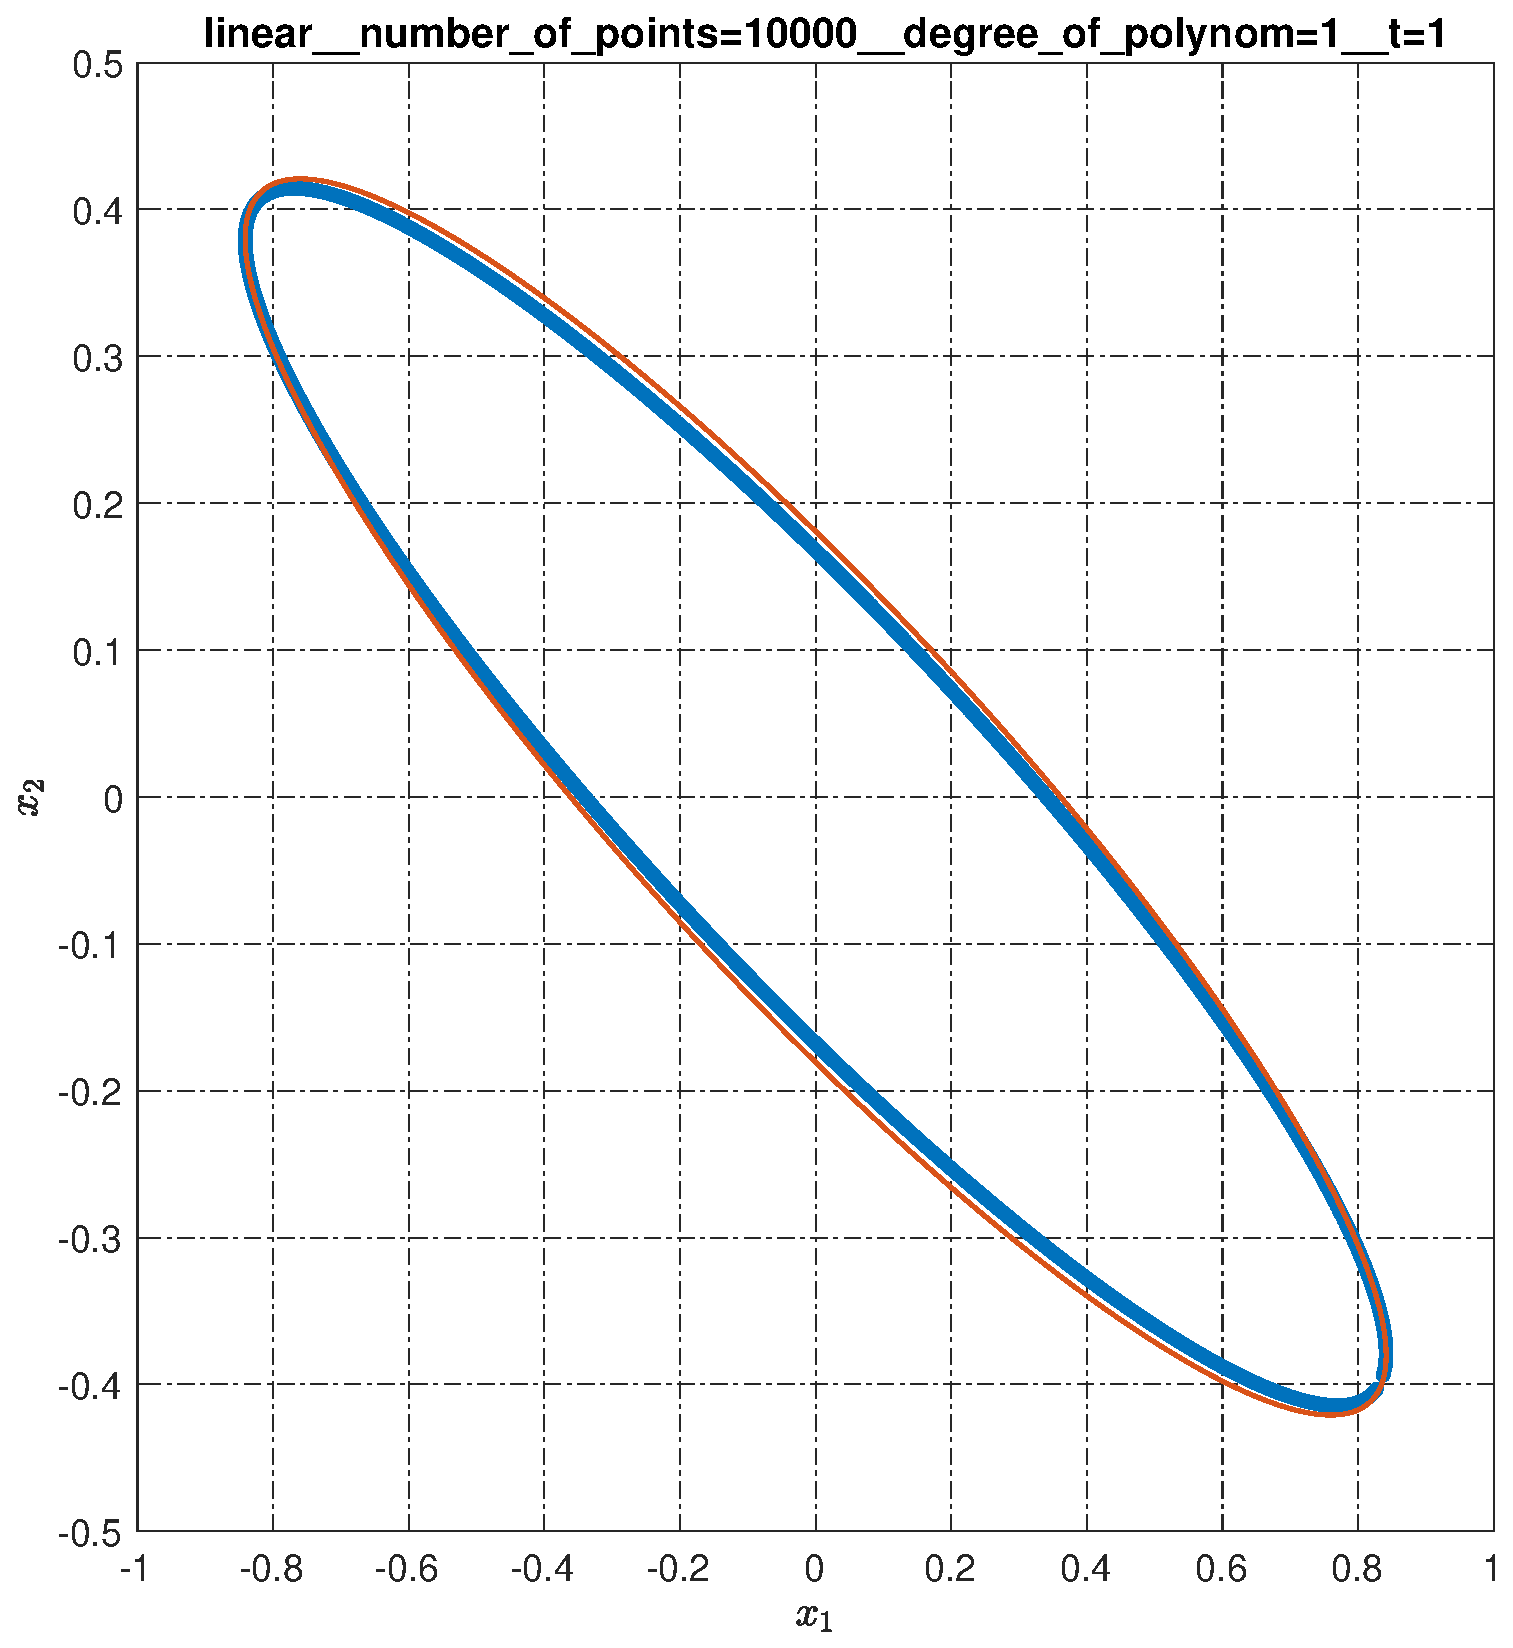
\includegraphics[width=\linewidth]{images/linear__number_of_points=10000__degree_of_polynom=1__t=1.eps}
 		\subcaption{$ N = 10^4 $, $ k = 1 $, $T = 1 $ }
 		 \label{fig:ap:linearN104k1T1} 
 	\end{minipage} 
 	\hfill
 	\begin{minipage}[b]{.3\linewidth} 
 		\small
 		\centering
 		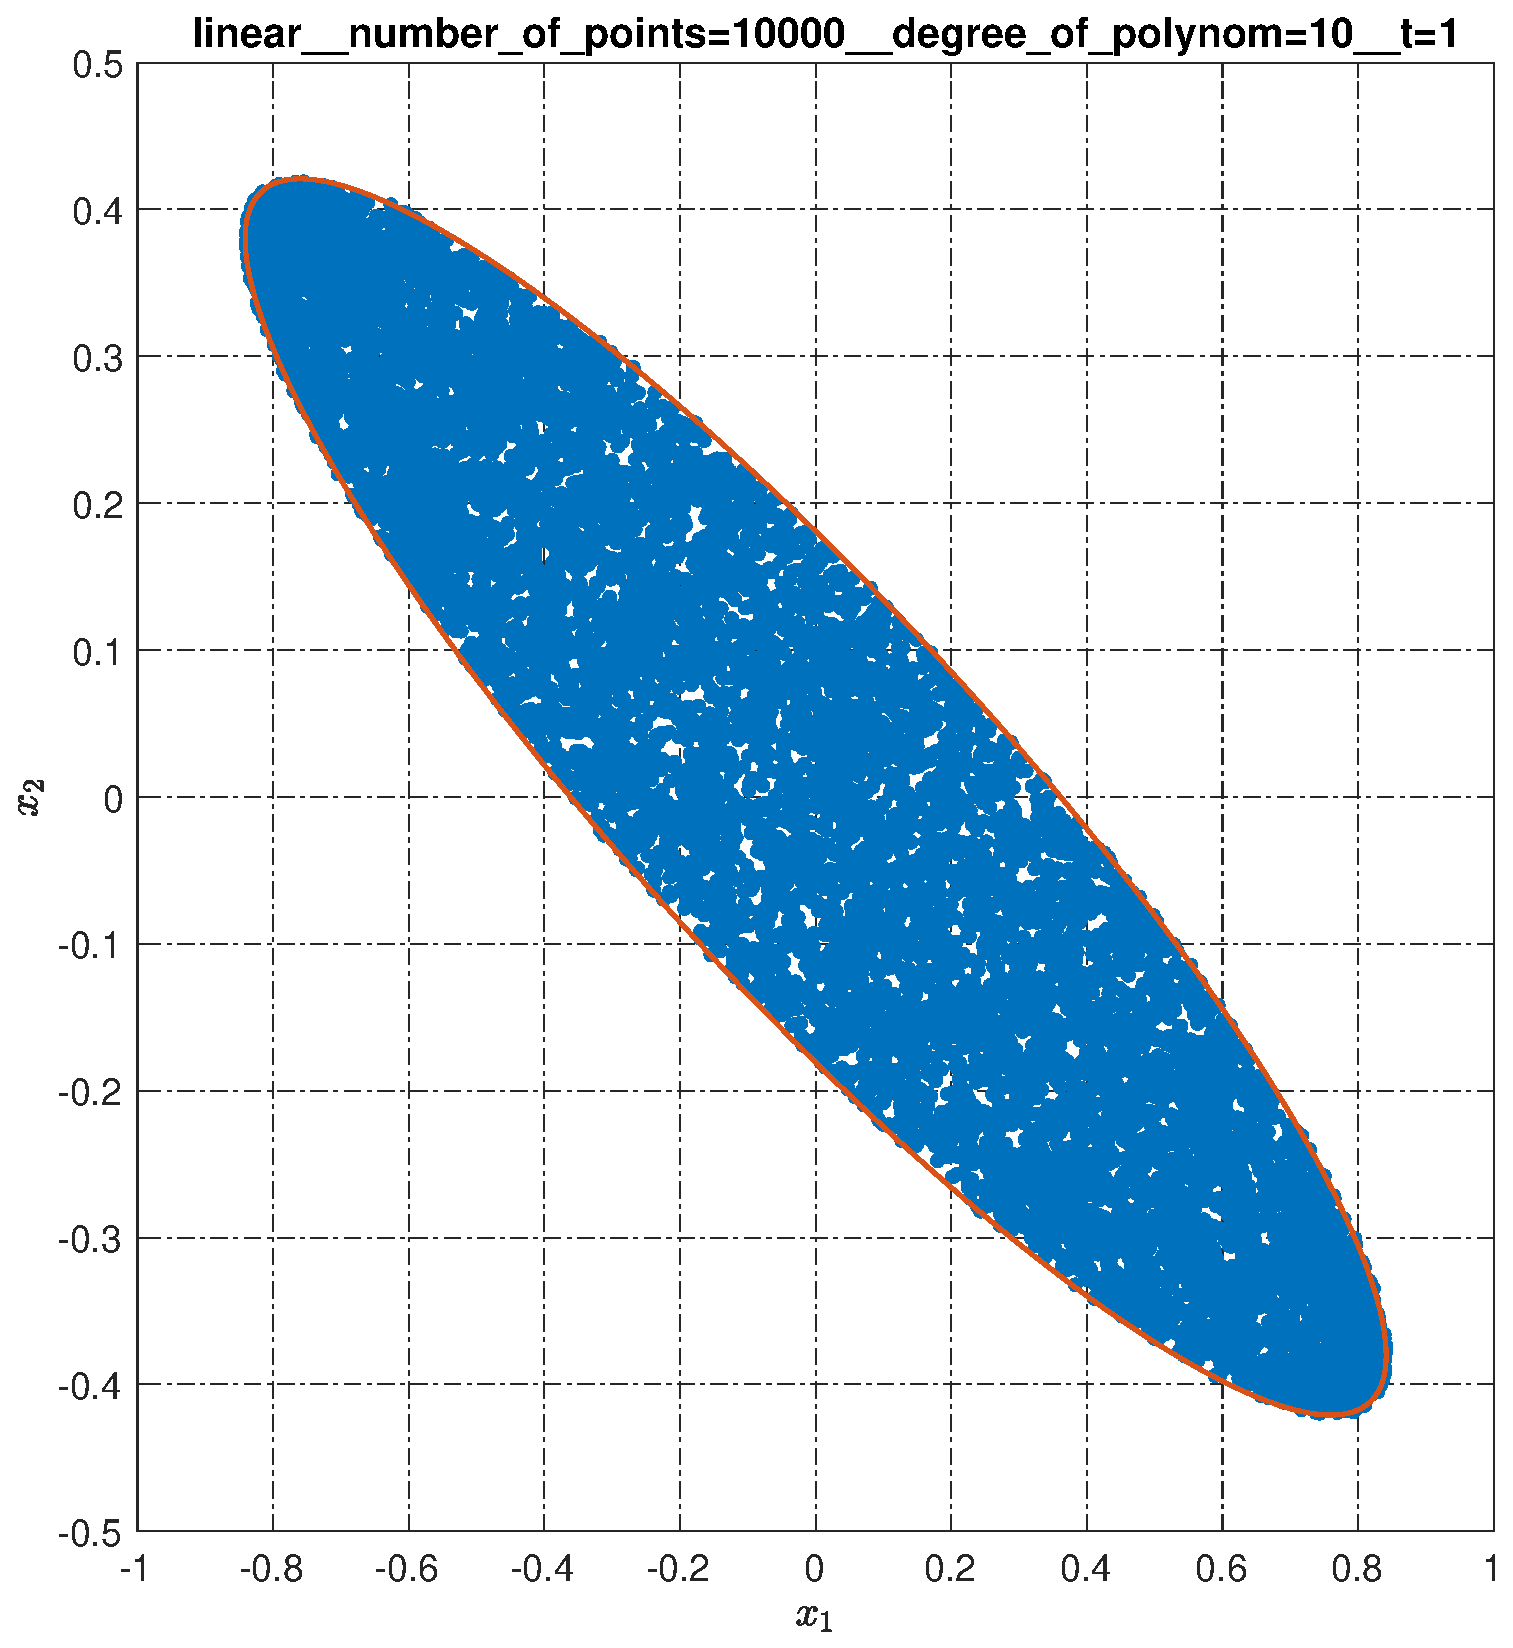
\includegraphics[width=\linewidth]{images/linear__number_of_points=10000__degree_of_polynom=10__t=1.eps}
 		\subcaption{$ N = 10^4 $, $ k = 10 $, $T = 1 $ }
 	\end{minipage} 
 	\vfill
 	\begin{minipage}[b]{.3\linewidth} 
 		\small
 		\centering 
 		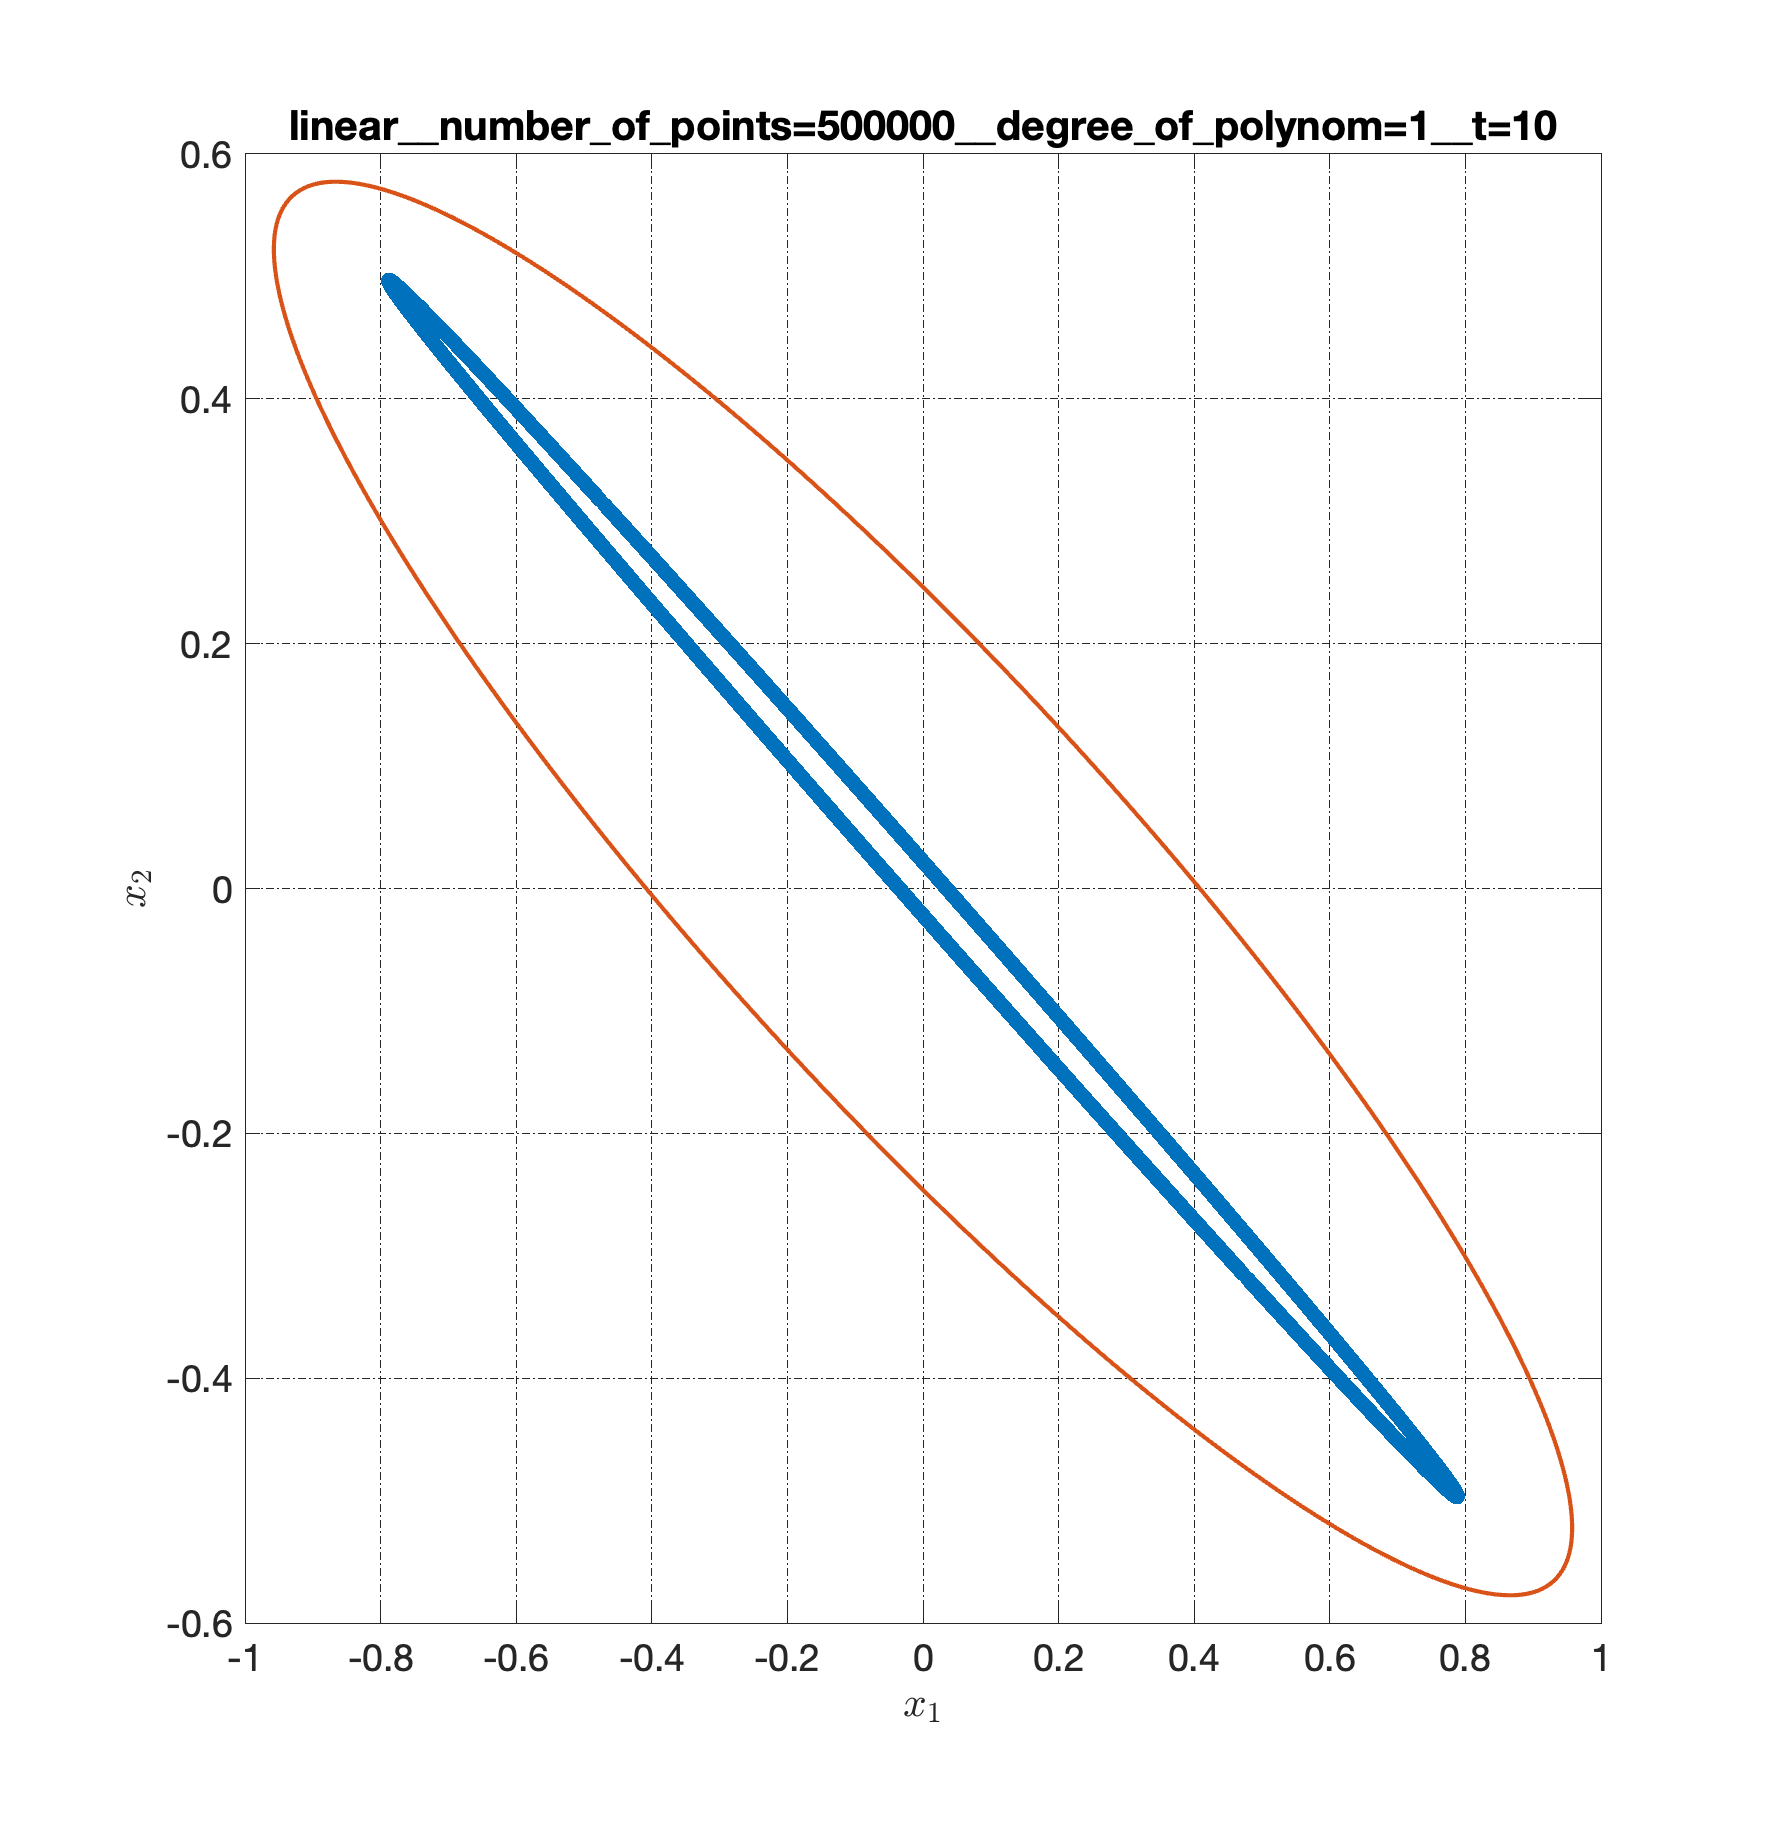
\includegraphics[width=\linewidth]{images/linear__number_of_points=500000__degree_of_polynom=1__t=10.eps}
 		\subcaption{$ N = 5\cdot 10^5 $, $ k = 1 $, $T = 10 $ }
 		\label{fig:ap:linearN5105k1T10}
 	\end{minipage}
 	\hfill
 	\begin{minipage}[b]{.3\linewidth} 
 		\small
 		\centering
 		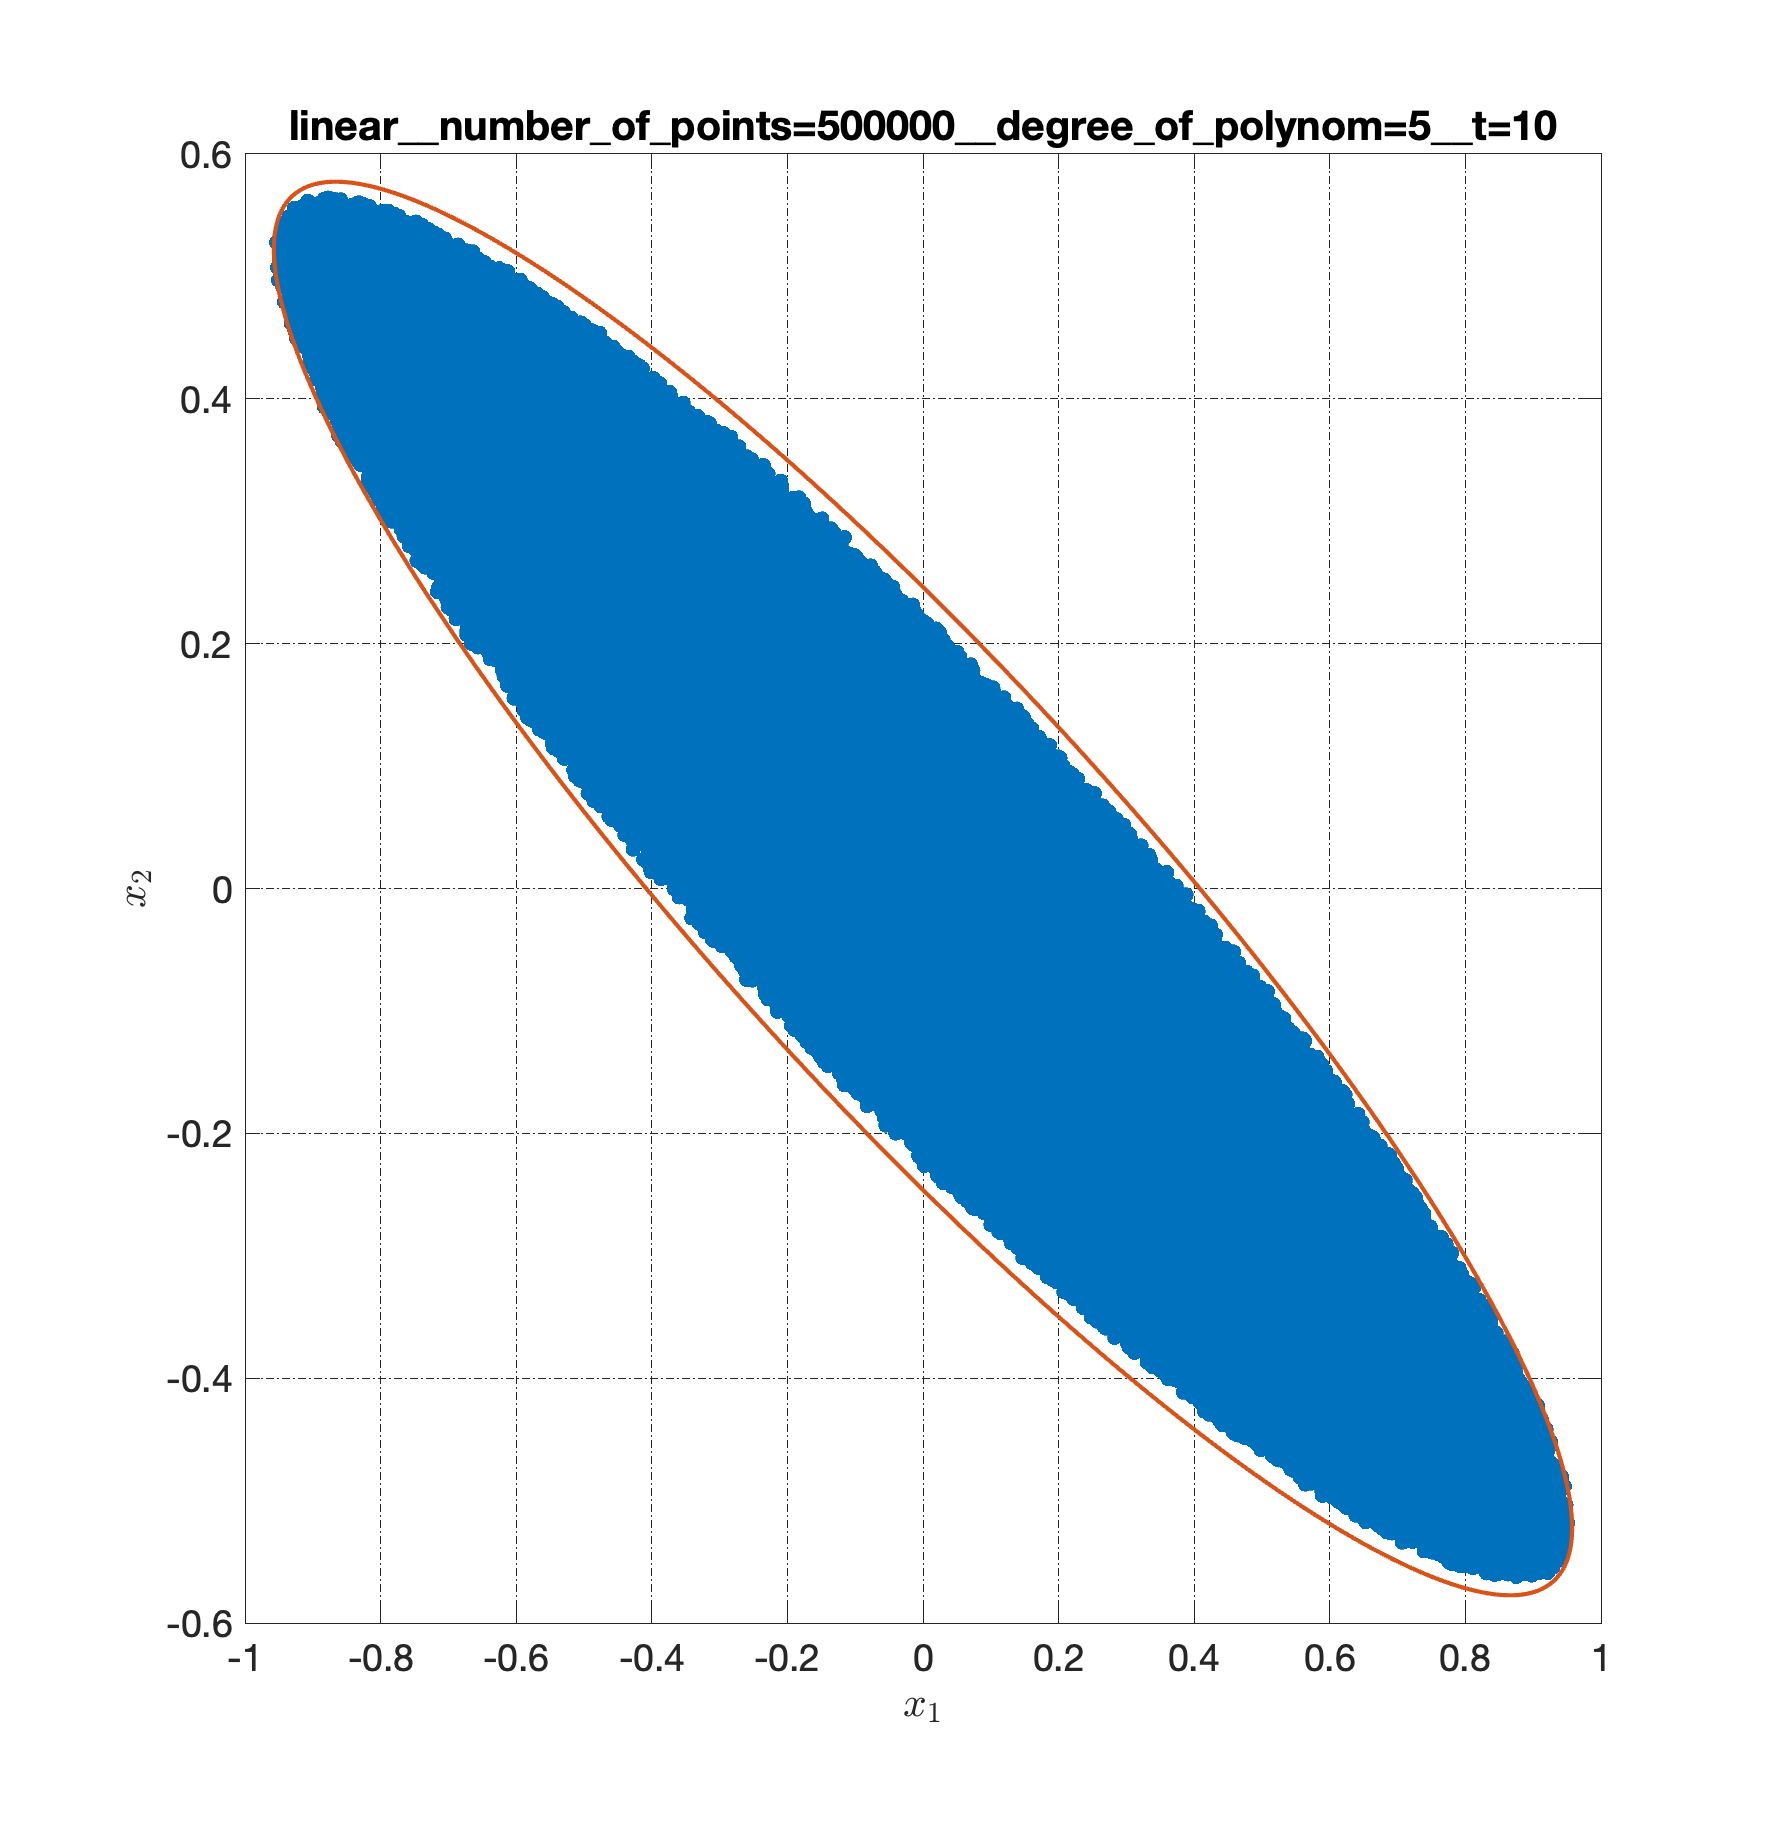
\includegraphics[width=\linewidth]{images/linear__number_of_points=500000__degree_of_polynom=5__t=10.eps}
 		\subcaption{$ N = 5\cdot 10^5 $, $ k = 5 $, $T = 10 $ } 
 	\end{minipage} 
 	\hfill
 	\begin{minipage}[b]{.3\linewidth} 
 		\small
 		\centering
 		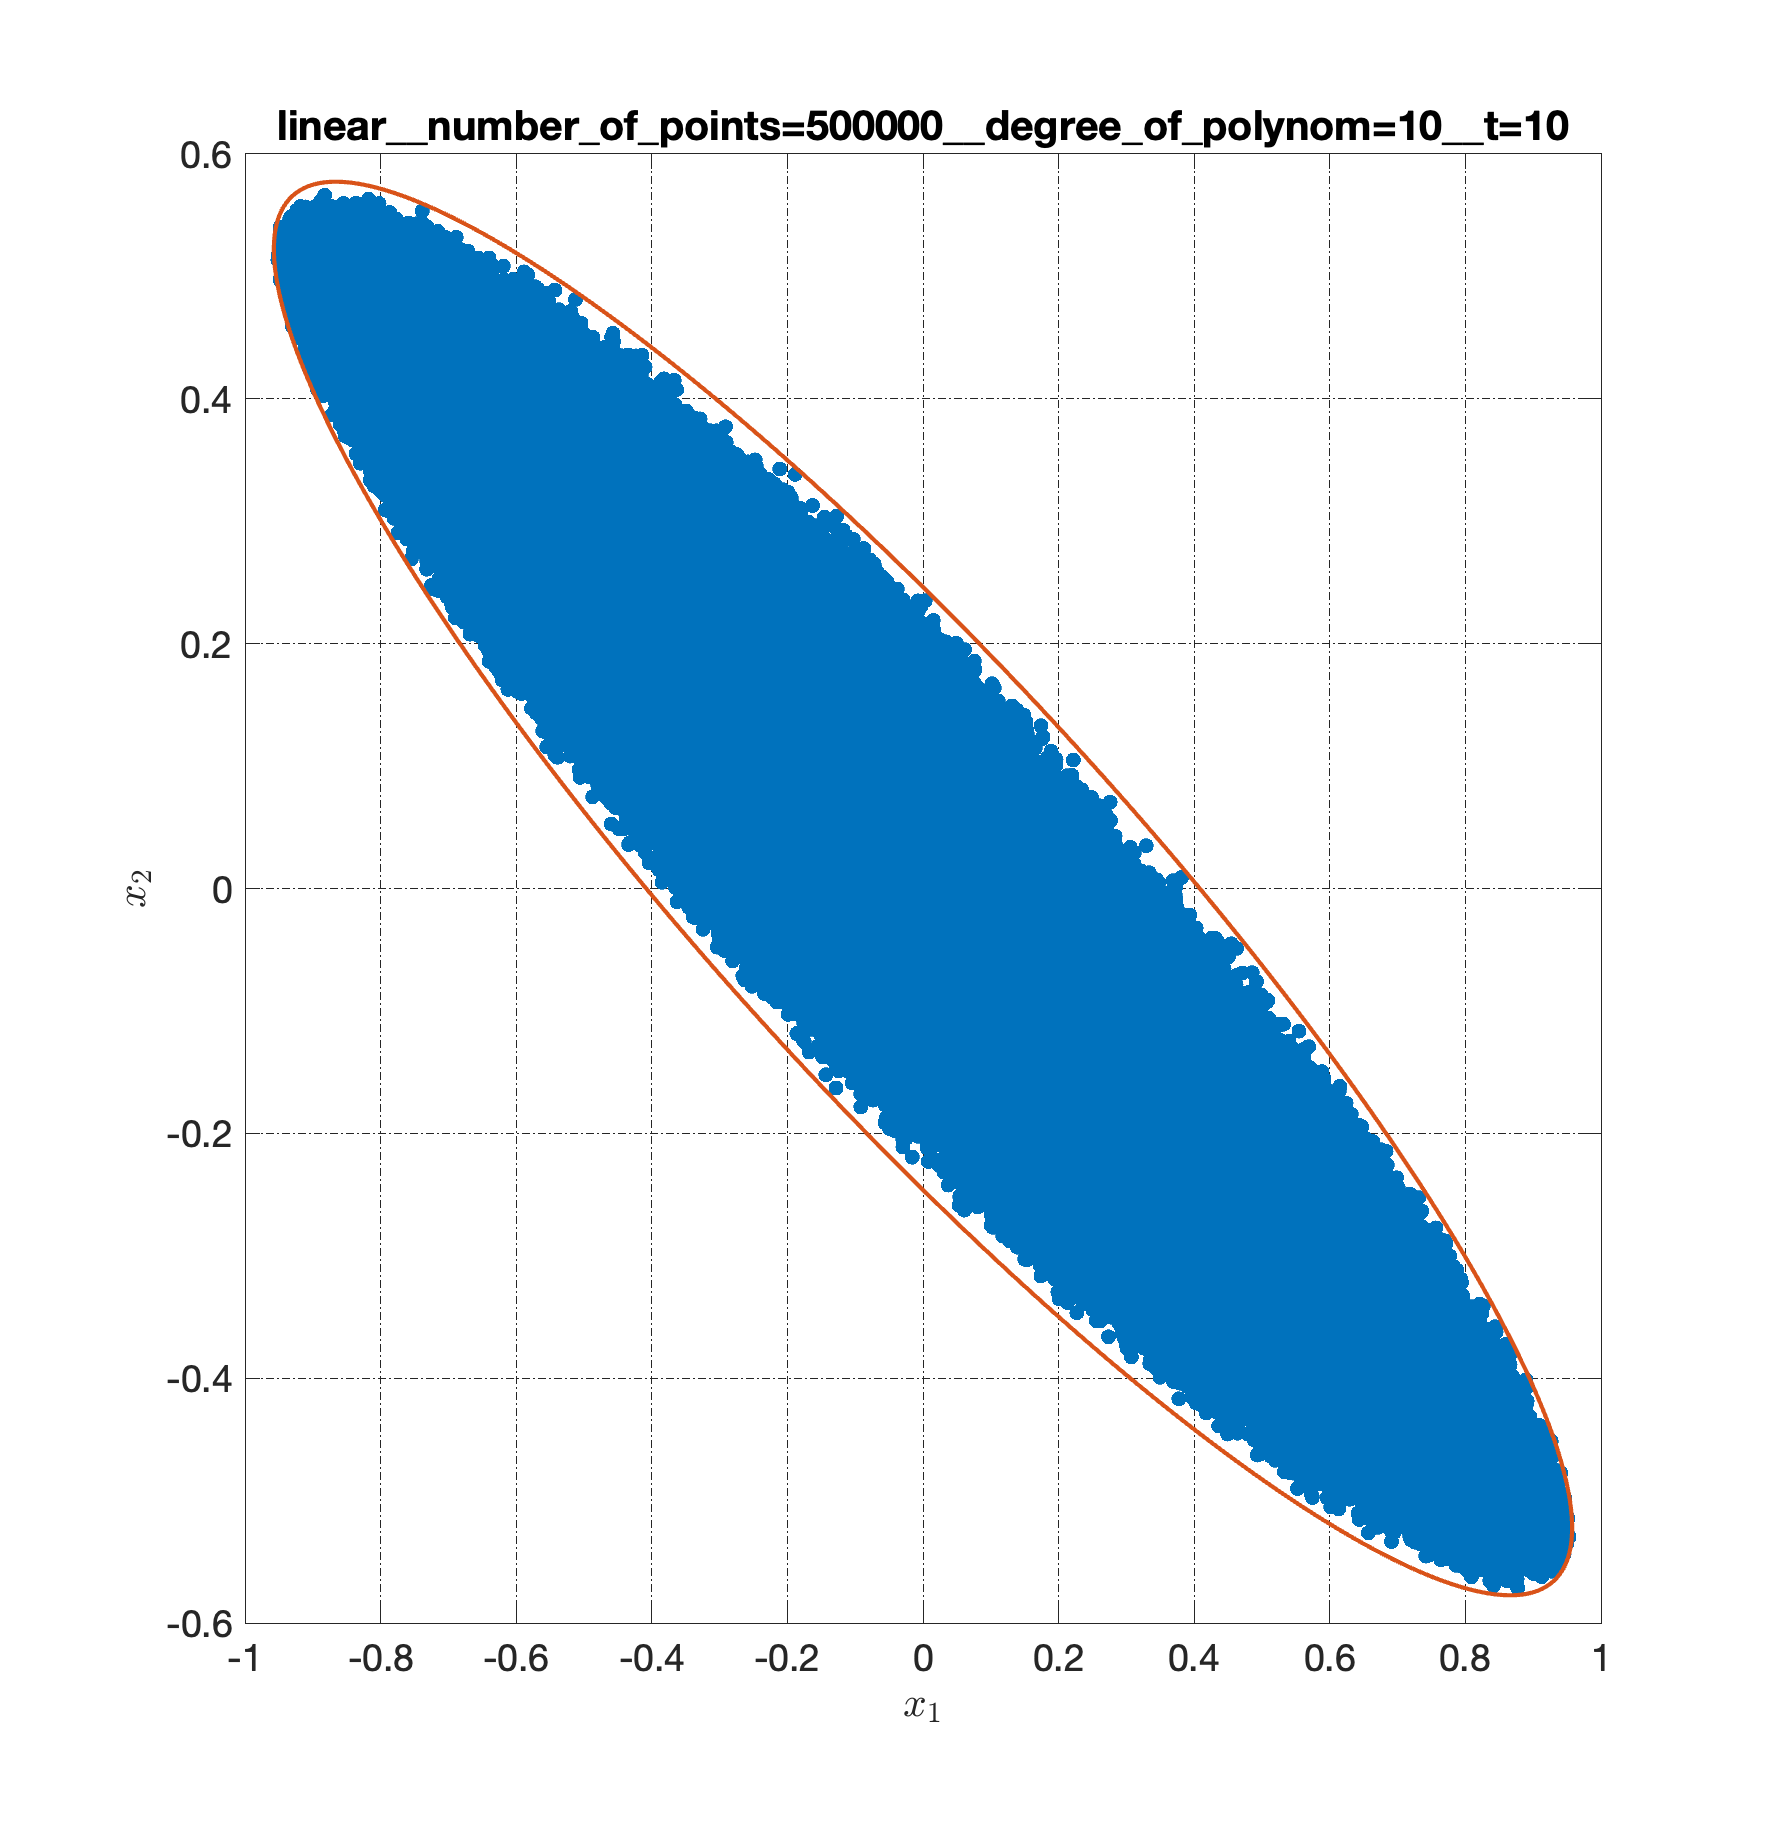
\includegraphics[width=\linewidth]{images/linear__number_of_points=500000__degree_of_polynom=10__t=10.eps}
 		\subcaption{$ N = 5\cdot 10^5 $, $ k = 10 $, $T = 10 $ } 
 	\end{minipage} 
 	\caption{Результаты численного эксперимента для системы \eqref{ap:linear_system1}.}\label{fig:ap:rs_linear1}
 \end{figure}
 
 \begin{figure}[ht!] 
 	 \hspace{-2.5ex}
 	\begin{minipage}[b]{.3\linewidth} 
 		\small
 		\centering 
 		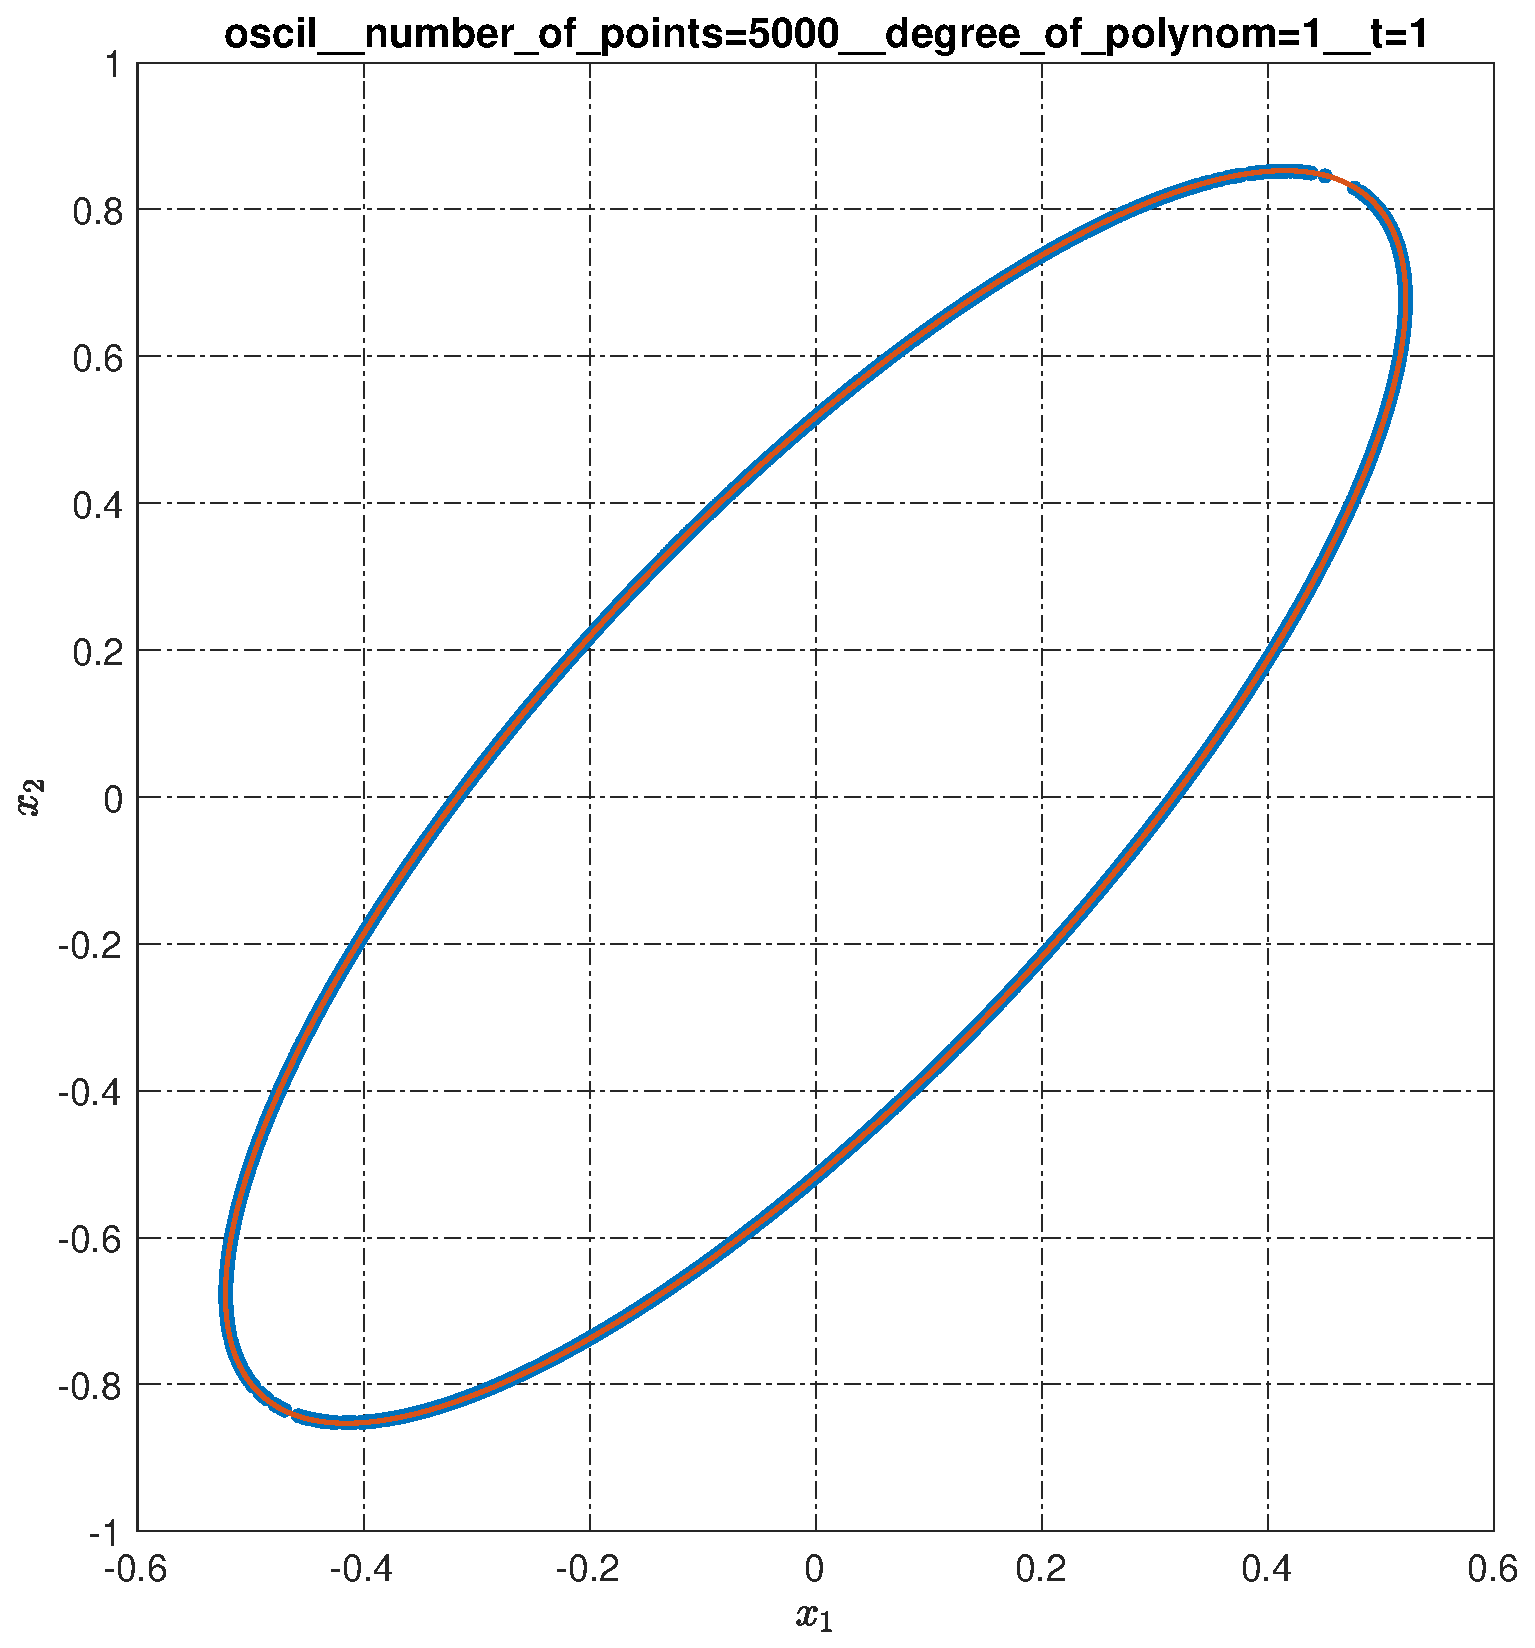
\includegraphics[width=\linewidth]{images/oscil__number_of_points=5000__degree_of_polynom=1__t=1.eps}
 		\subcaption{$ N = 5\cdot10^3 $, $ k = 1 $, $ t = 1 $ }
 		\label{fig:ap:oscilN5103k1T1} 
 	\end{minipage}
 	\hfill
 	\begin{minipage}[b]{.3\linewidth} 
 		\small
 		\centering
 		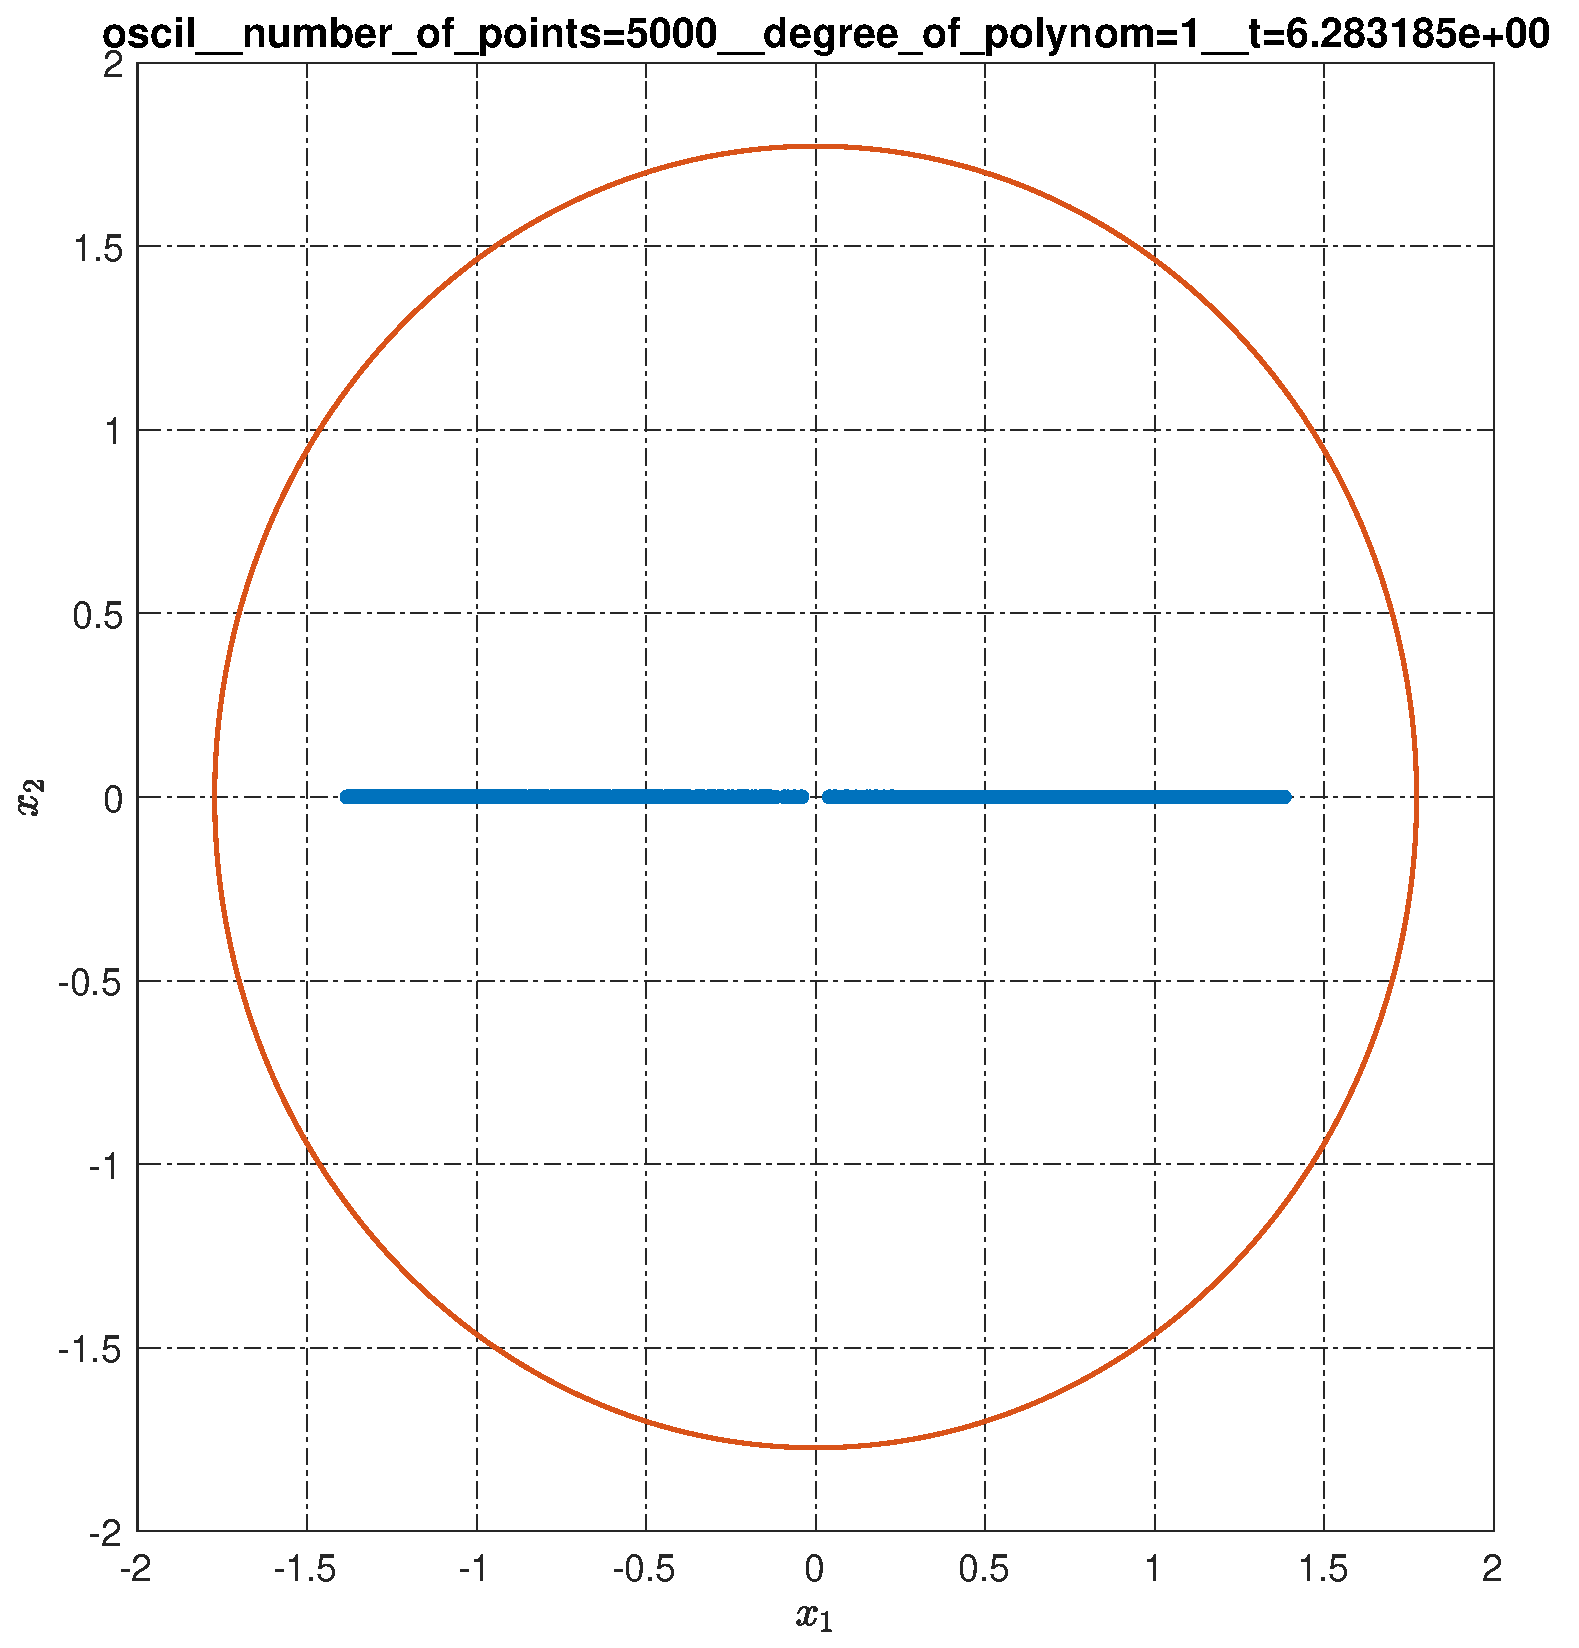
\includegraphics[width=\linewidth]{images/oscil__number_of_points=5000__degree_of_polynom=1__t=2pi.eps}
 		\subcaption{$ N = 5\cdot10^3 $, $ k = 1 $, $ t = 2\pi $}
 		\label{fig:ap:oscilN5103k1T2pi}
 	\end{minipage} 
 	\hfill
 	\begin{minipage}[b]{.3\linewidth} 
 		\small
 		\centering
 		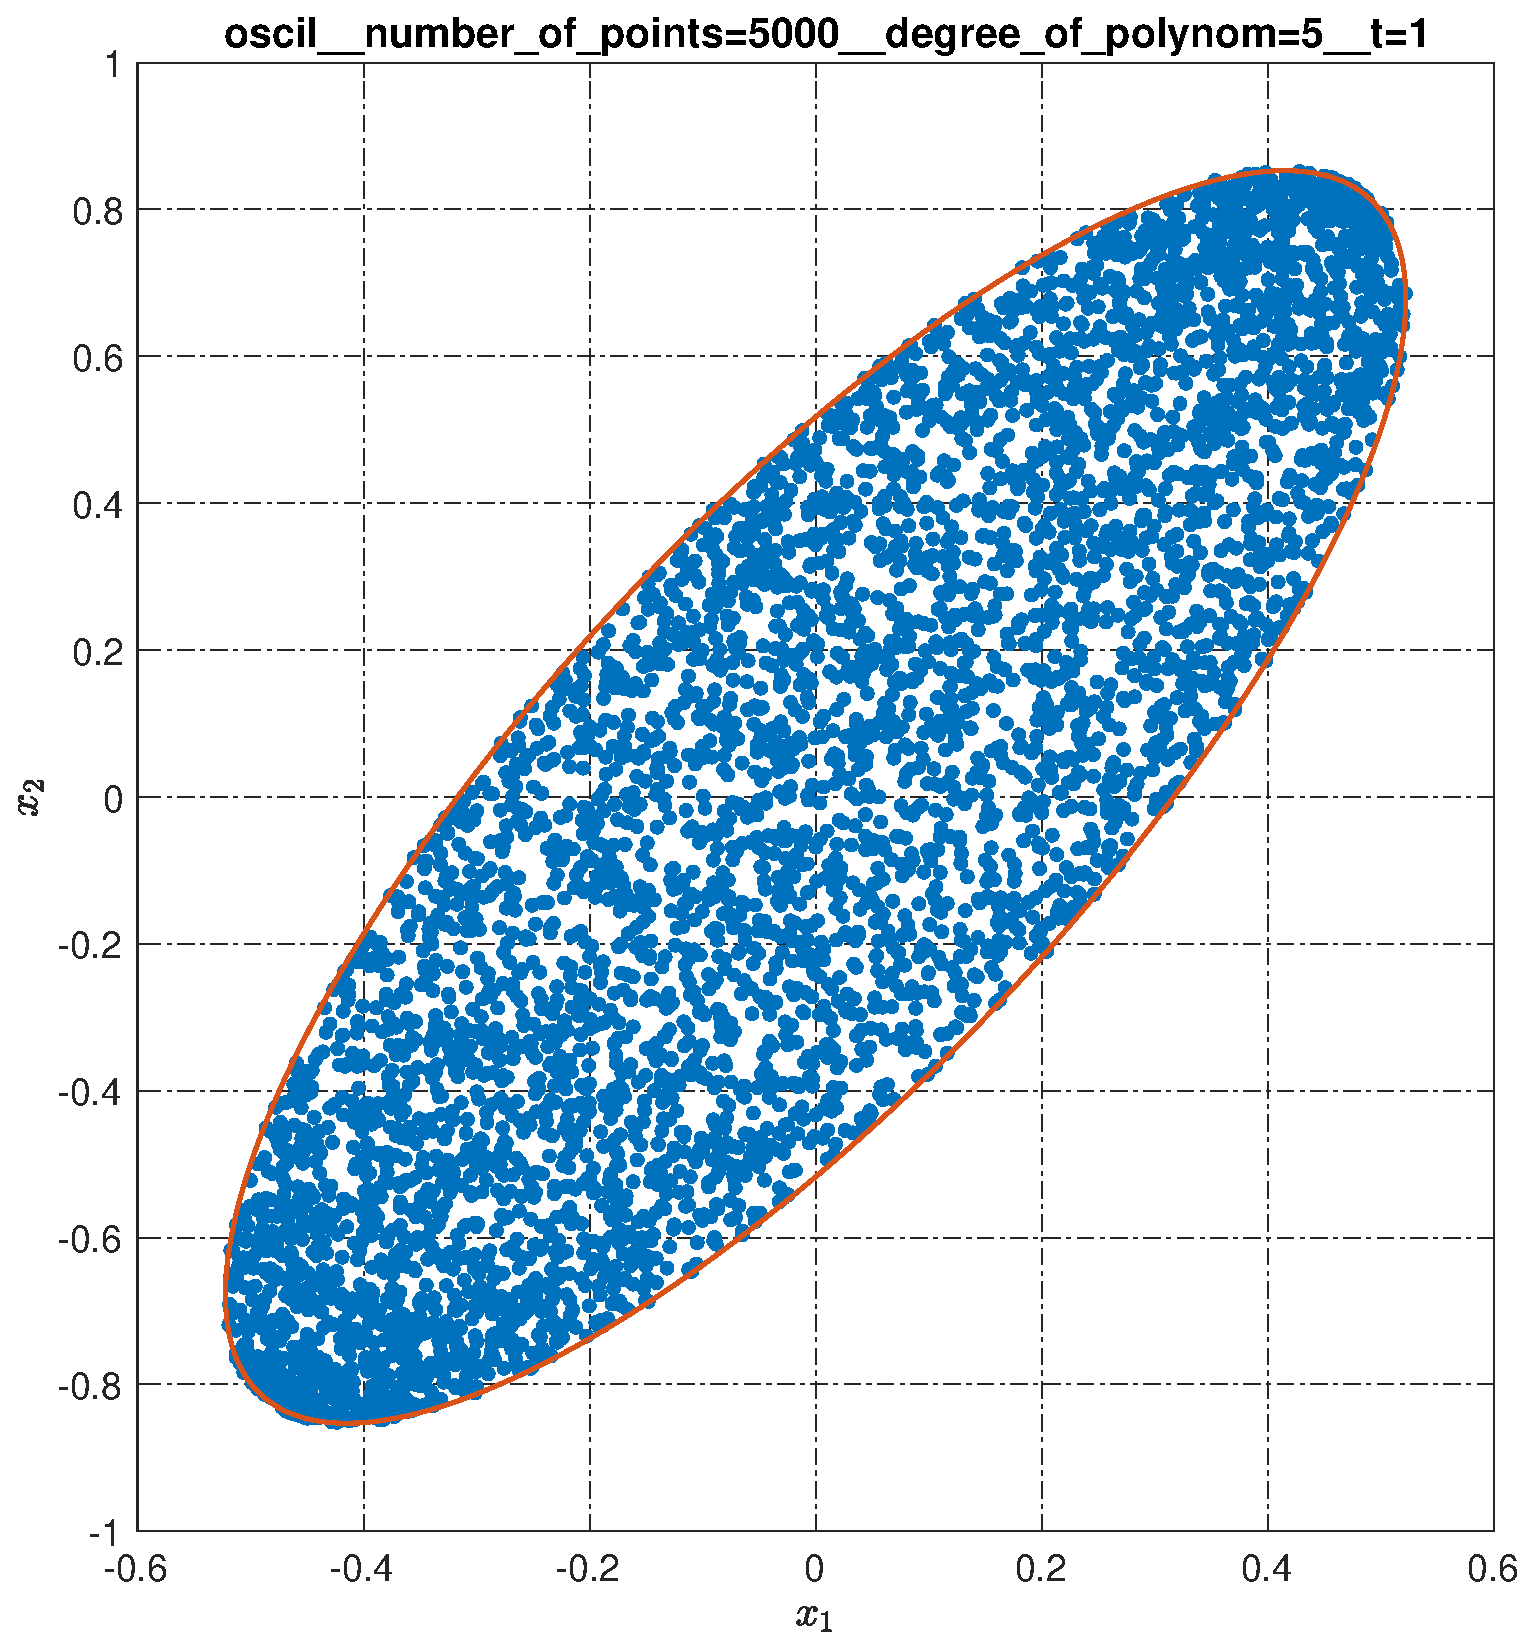
\includegraphics[width=\linewidth]{images/oscil__number_of_points=5000__degree_of_polynom=5__t=1.eps}
 		\subcaption{$ N = 5\cdot10^3 $, $ k = 5 $, $ t = 1 $}
 	\end{minipage} 
 	\vfill
 	\hspace{-2.5ex}
 	\begin{minipage}[b]{.3\linewidth} 
 		\small
 		\centering 
 		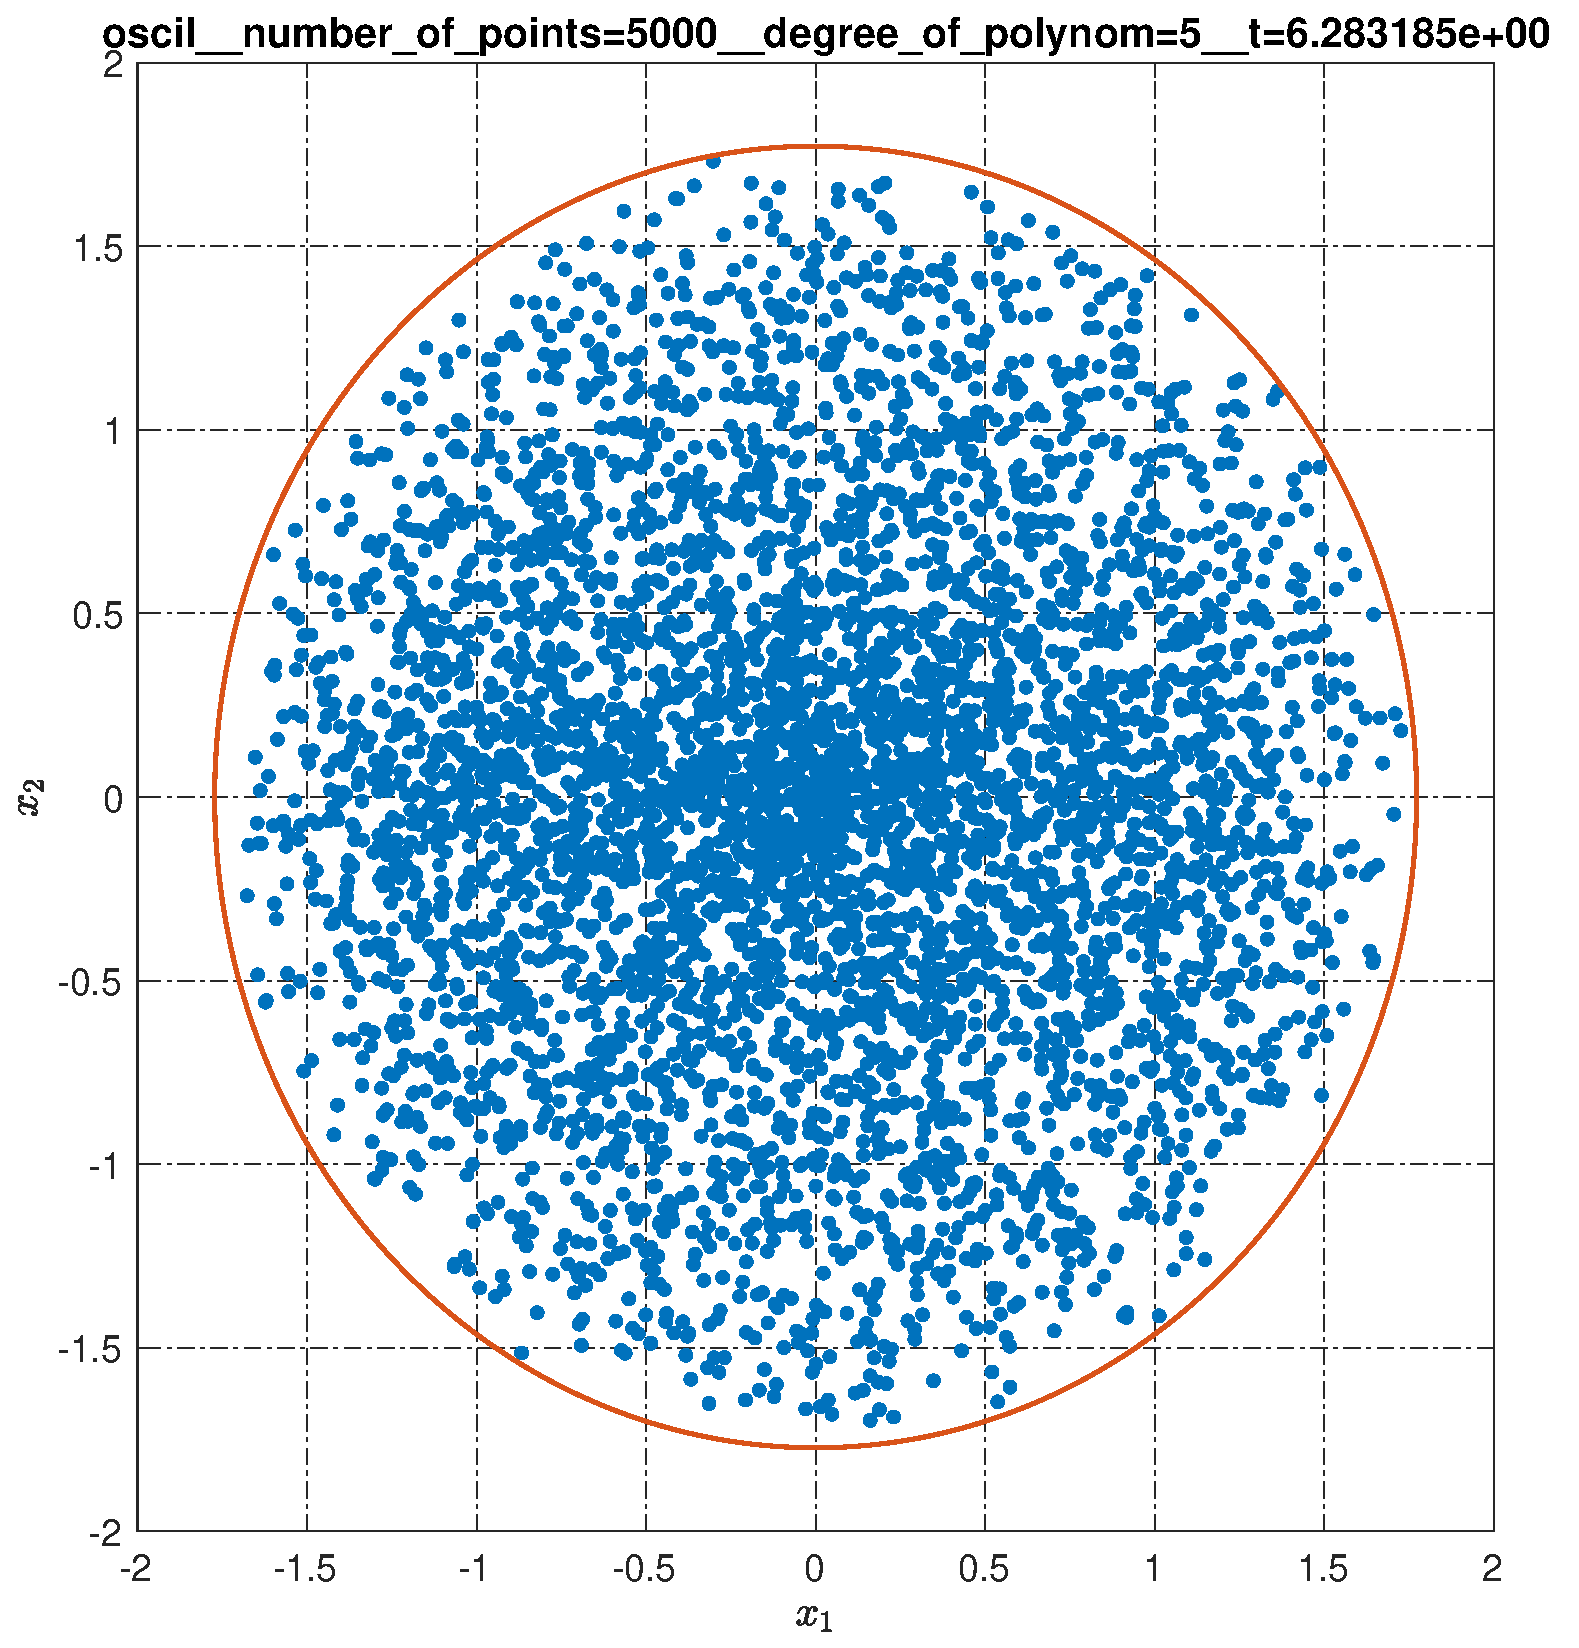
\includegraphics[width=\linewidth]{images/oscil__number_of_points=5000__degree_of_polynom=5__t=2pi.eps}
 		\subcaption{$ N = 5\cdot10^3 $, $ k = 5 $, $ t = 2\pi $ }
 		\label{fig:ap:oscilN5103k5T2pi}
 	\end{minipage}
 	\hfill
 	\begin{minipage}[b]{.3\linewidth} 
 		\small
 		\centering
 		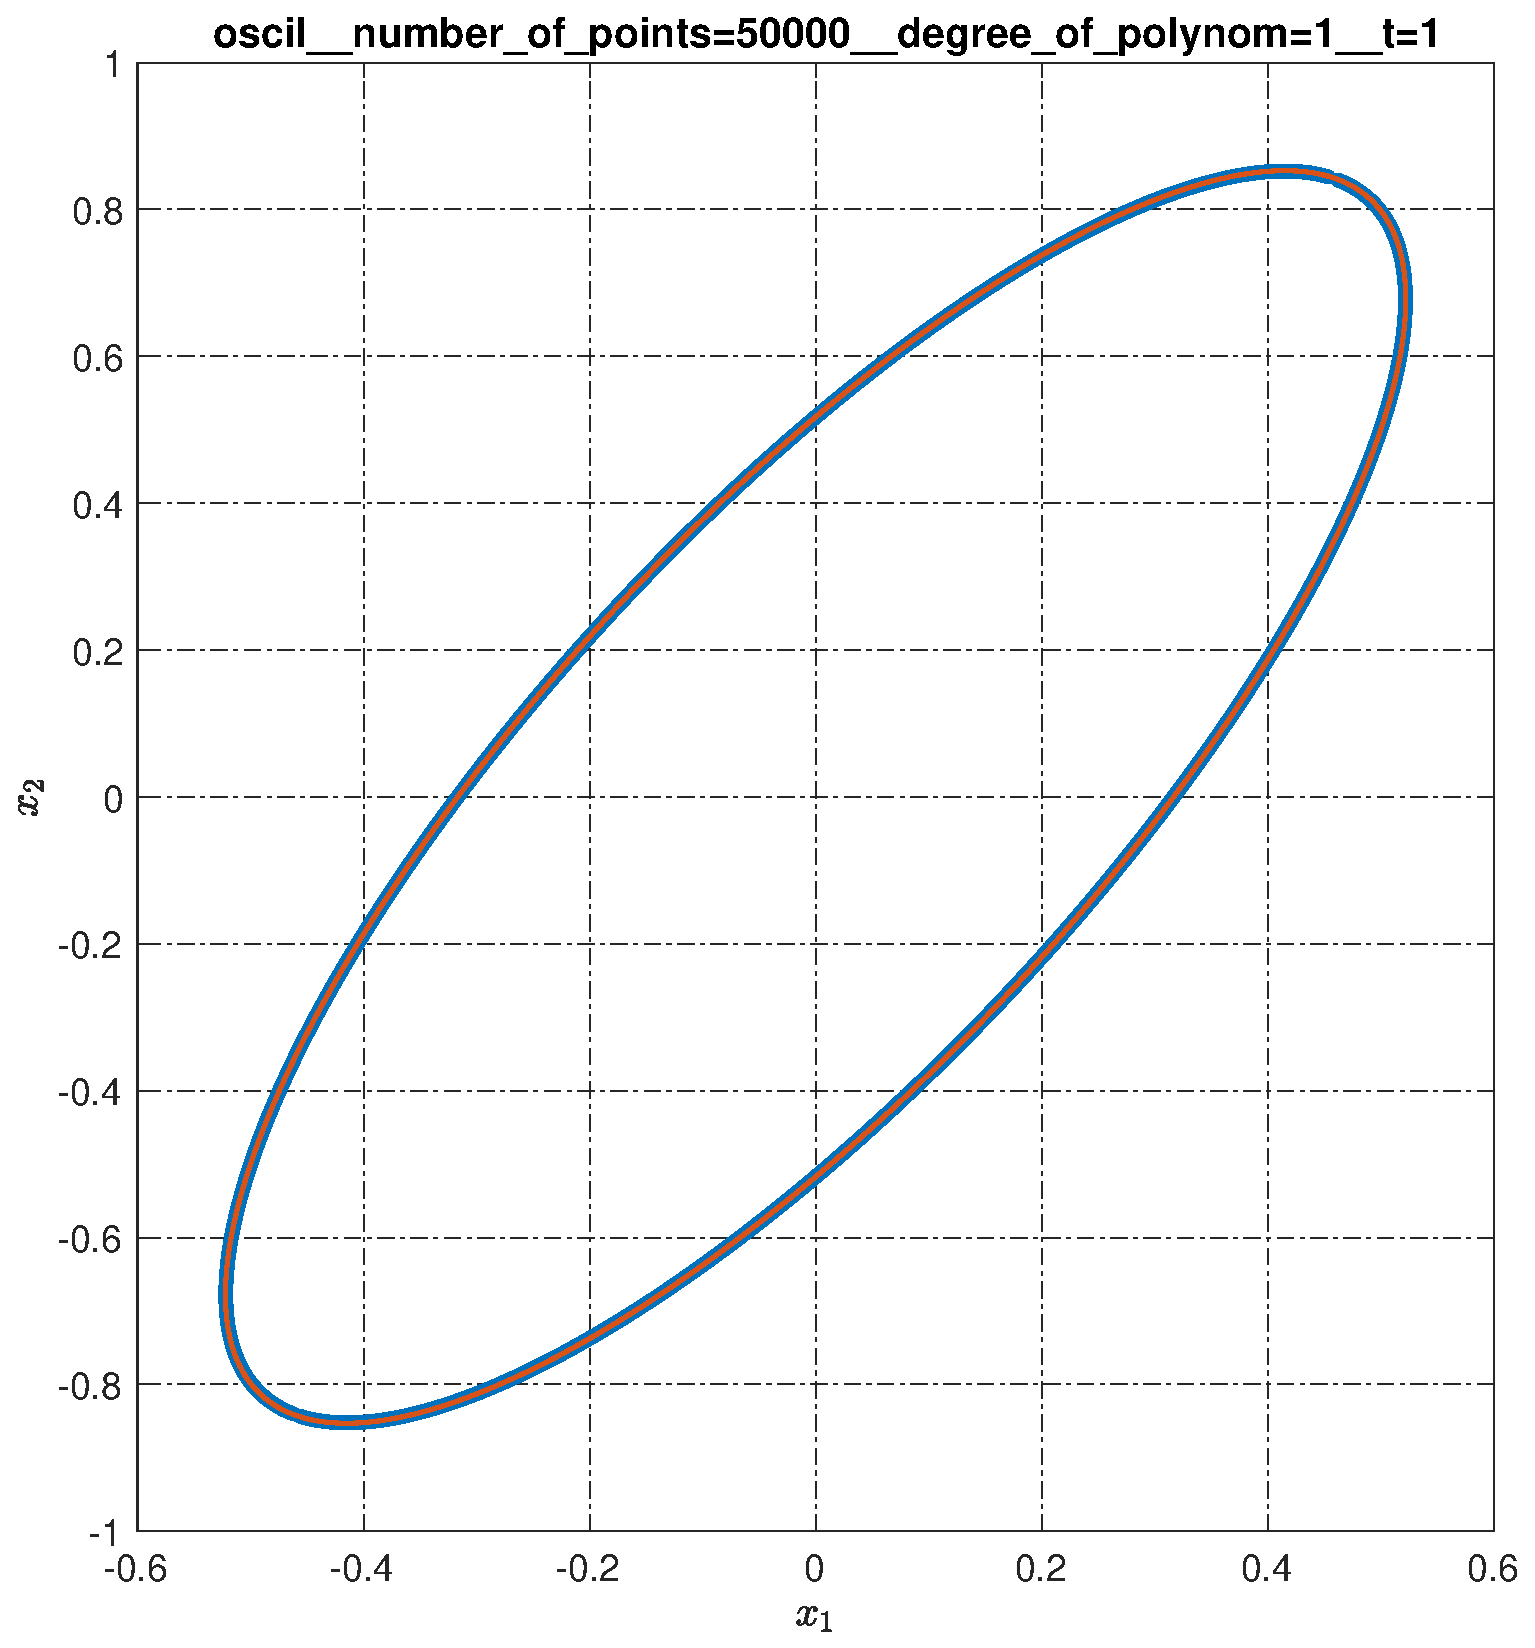
\includegraphics[width=\linewidth]{images/oscil__number_of_points=50000__degree_of_polynom=1__t=1.eps}
 		\subcaption{$ N = 5\cdot10^4 $, $ k = 1 $, $ t = 1 $}
 		\label{fig:ap:oscilN5104k1T1}
 	\end{minipage} 
 	\hfill
 	\begin{minipage}[b]{.3\linewidth} 
 		\small
 		\centering
 		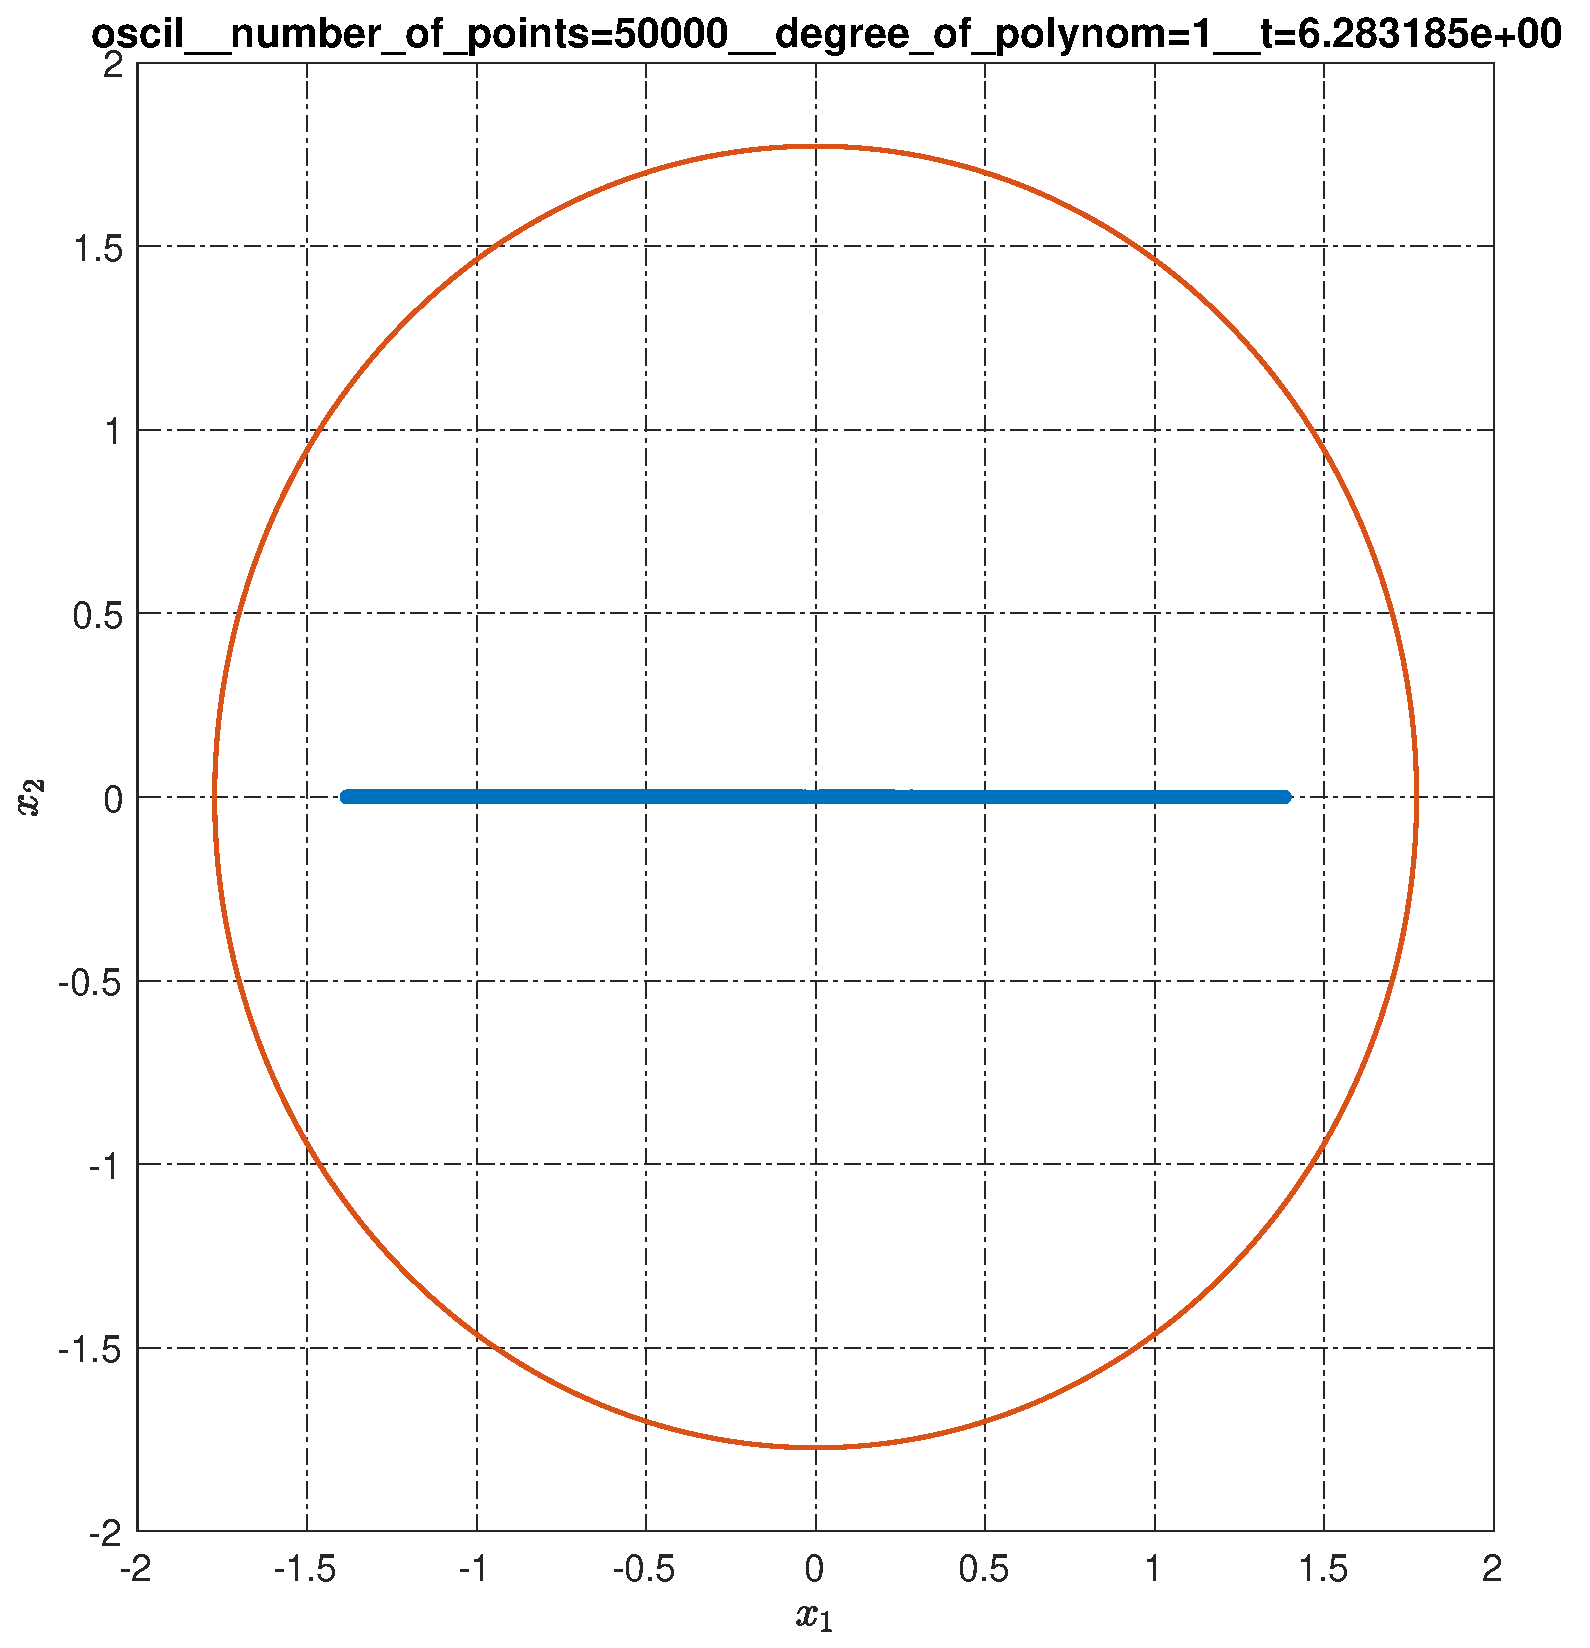
\includegraphics[width=\linewidth]{images/oscil__number_of_points=50000__degree_of_polynom=1__t=2pi.eps}
 		\subcaption{$ N = 5\cdot10^4 $, $ k = 1 $, $ t = 2\pi $ }
 		\label{fig:ap:oscilN5104k1T2pi}
 	\end{minipage} 
 	\vfill
 	\hspace{-2.5ex}
 	\begin{minipage}[b]{.3\linewidth} 
 		\small
 		\centering 
 		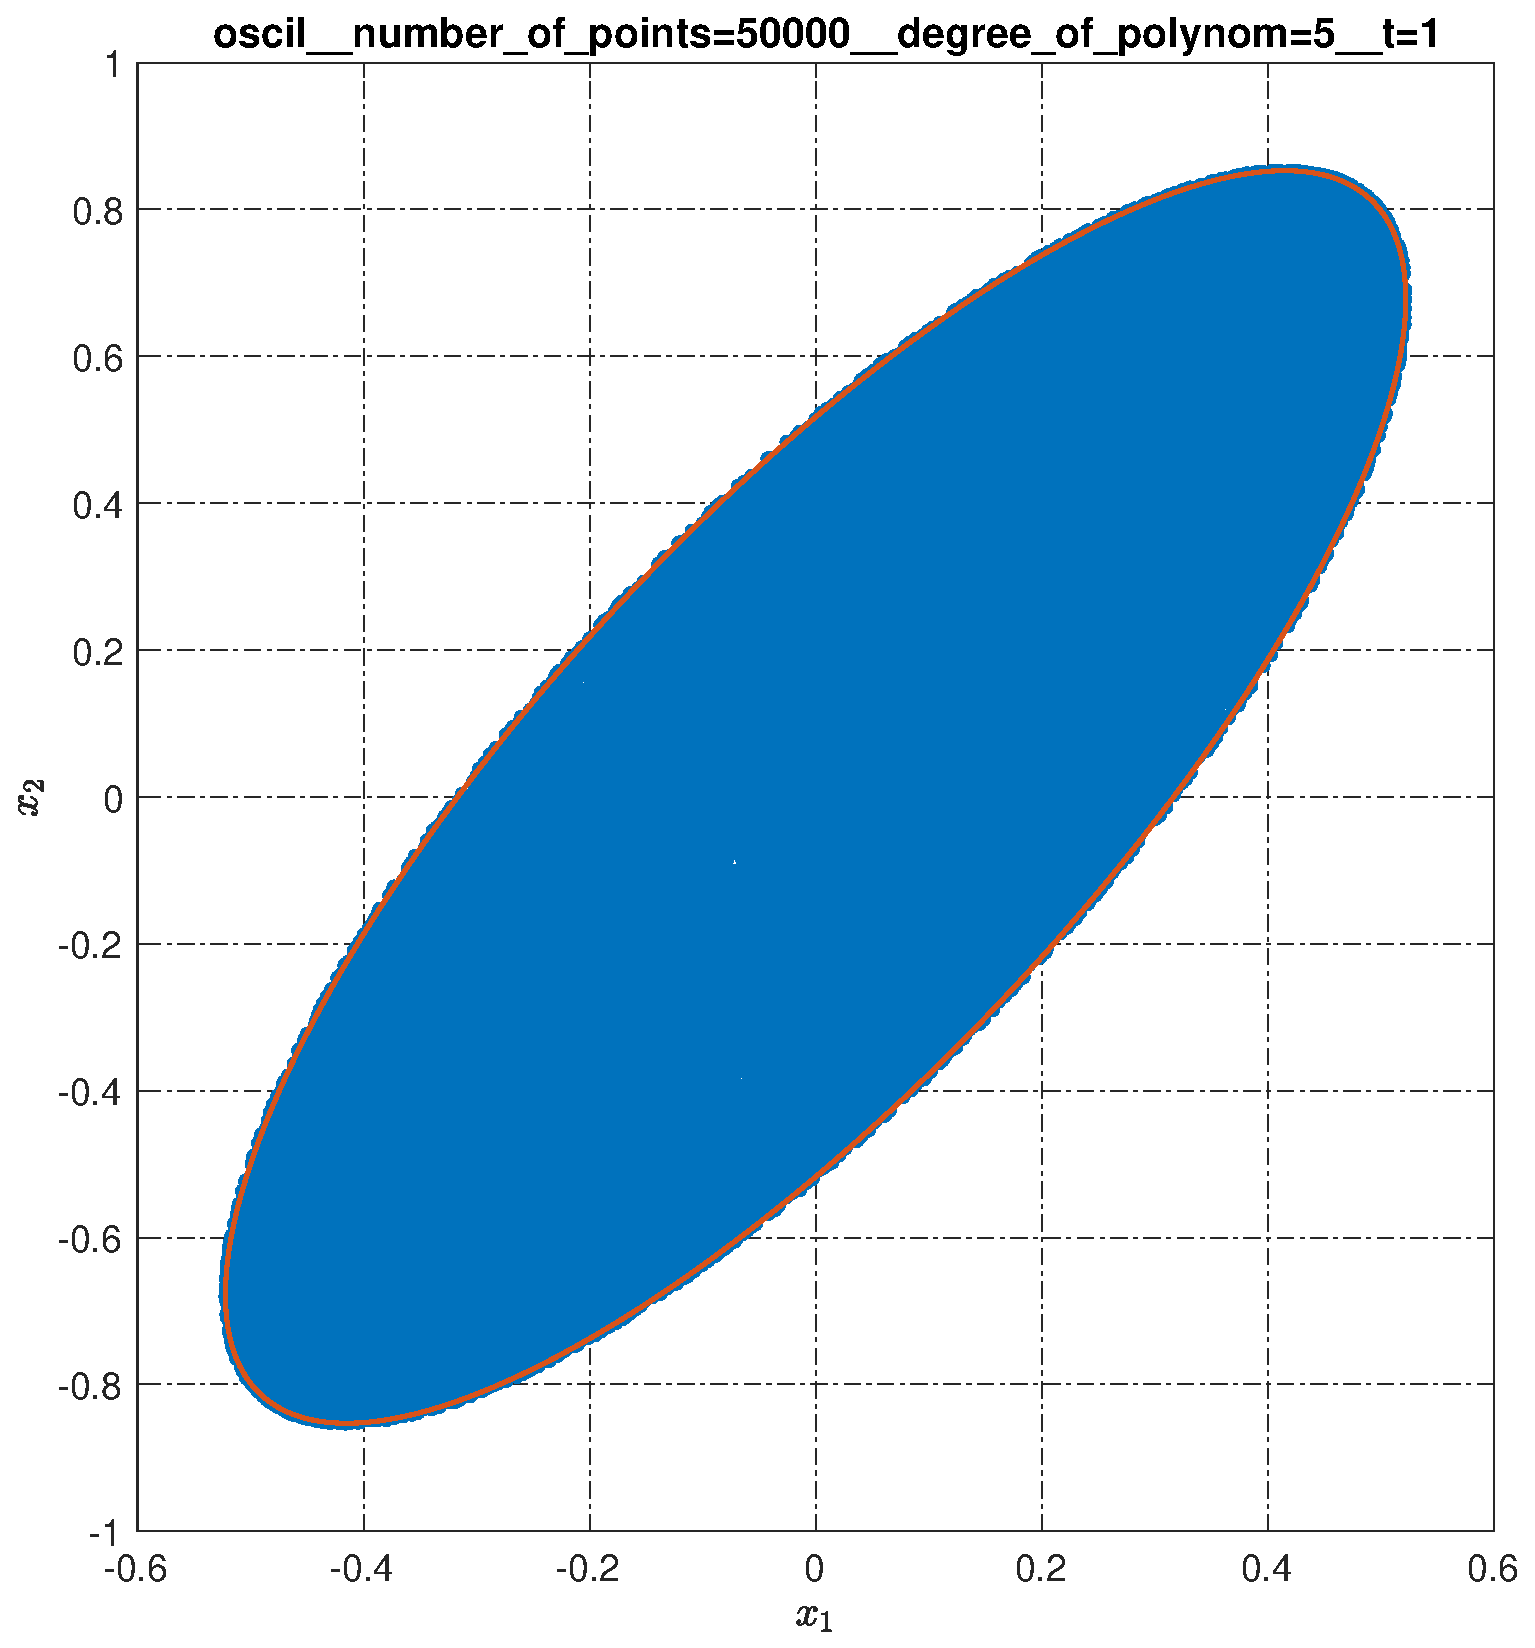
\includegraphics[width=\linewidth]{images/oscil__number_of_points=50000__degree_of_polynom=5__t=1.eps}
 		\subcaption{$ N = 5\cdot10^4 $, $ k = 5 $, $ t = 1 $}
 	\end{minipage}
 	\hfill
 	\begin{minipage}[b]{.3\linewidth} 
 		\small
 		\centering
 		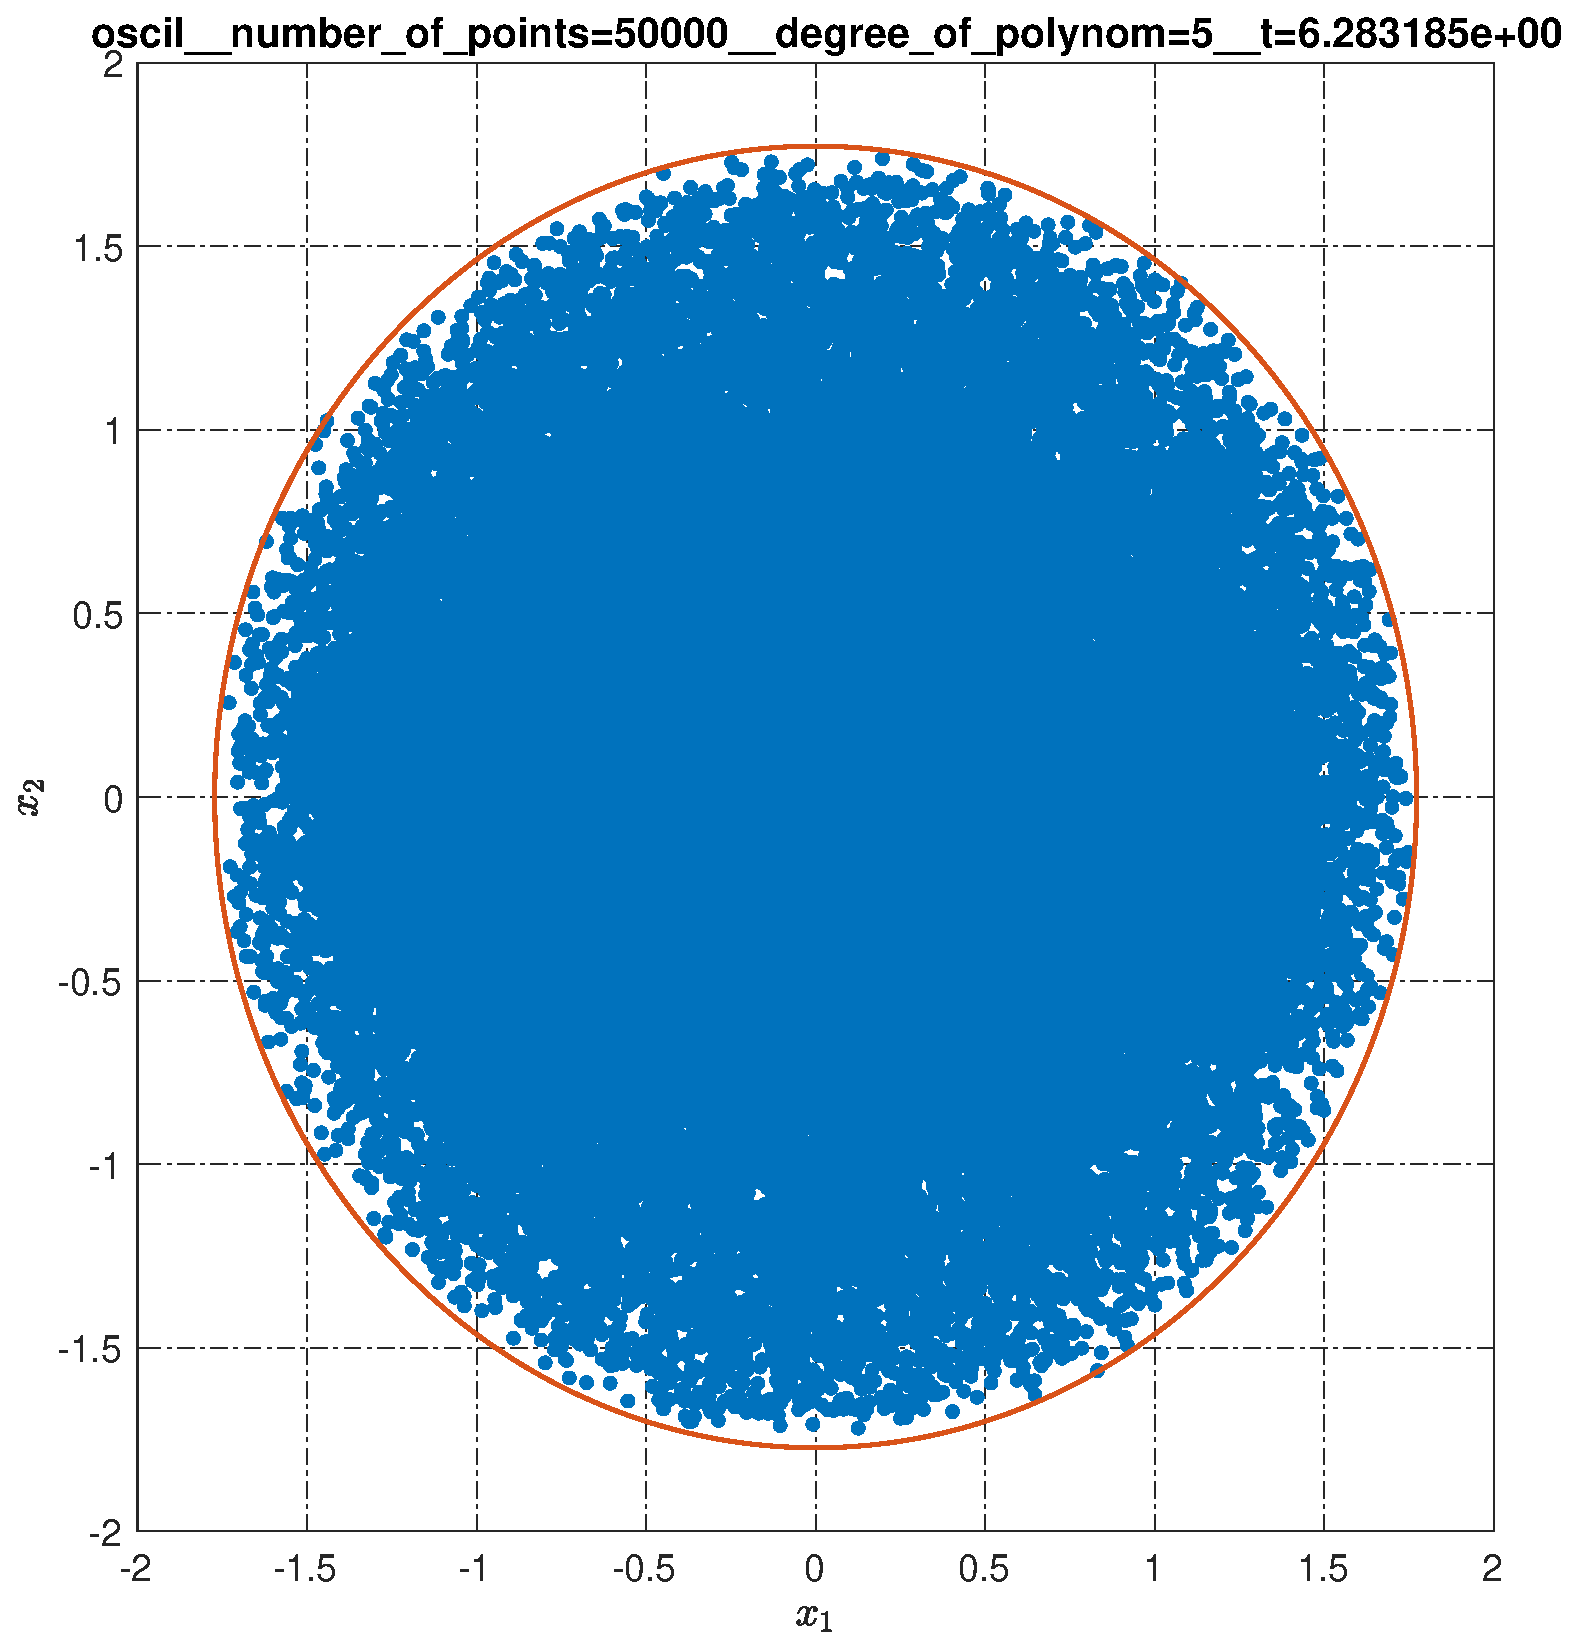
\includegraphics[width=\linewidth]{images/oscil__number_of_points=50000__degree_of_polynom=5__t=2pi.eps}
 		\subcaption{$ N = 5\cdot10^4 $, $ k = 5 $, $ t = 2\pi $ } 
 		\label{fig:ap:oscilN5104k5T2pi}
 	\end{minipage} 
 	\hfill
 	\begin{minipage}[b]{.3\linewidth} 
 		\small
 		\centering
 		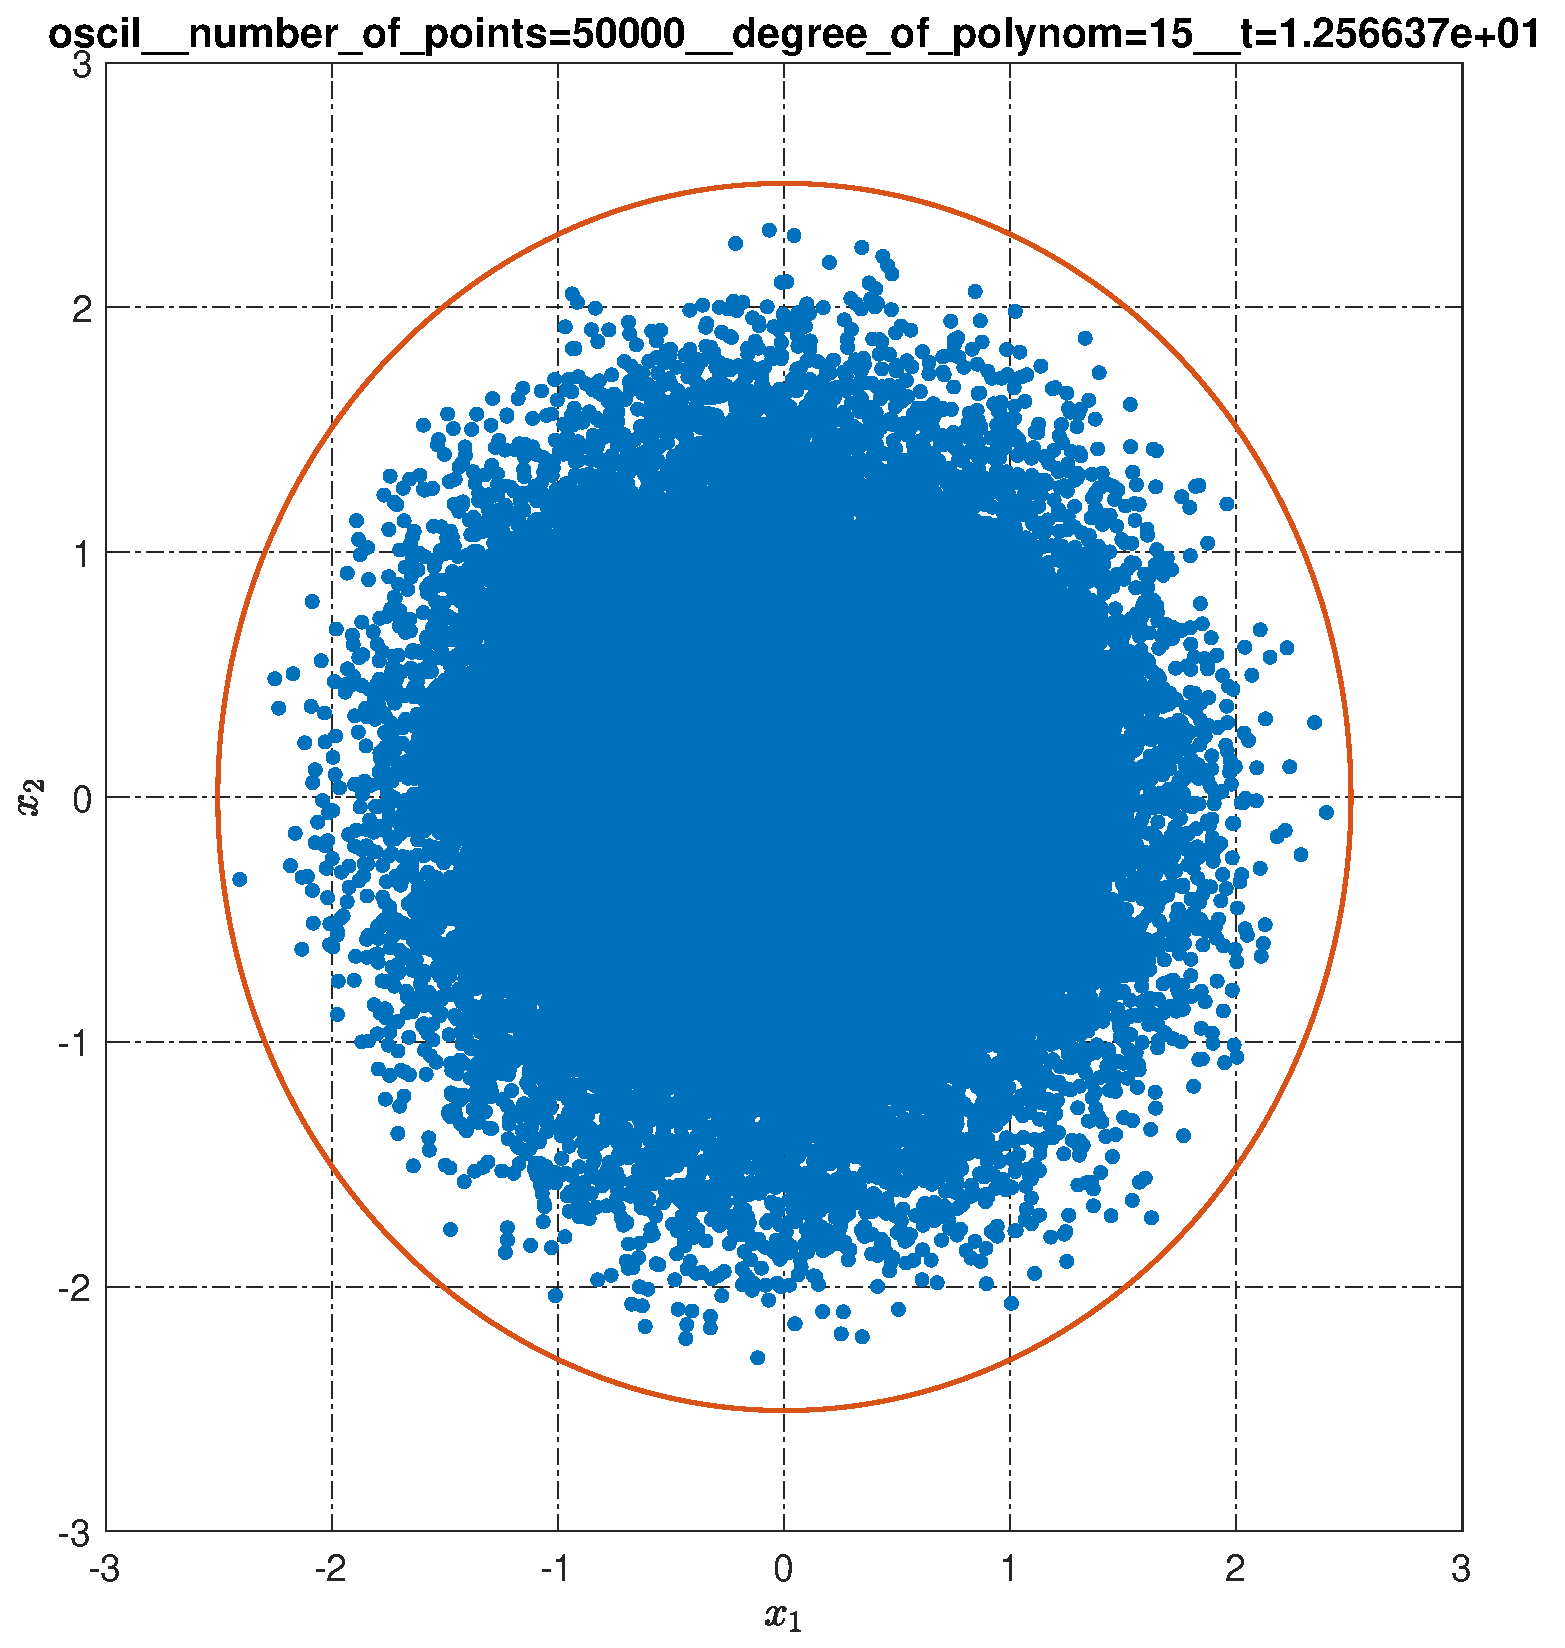
\includegraphics[width=\linewidth]{images/oscil__number_of_points=50000__degree_of_polynom=15__t=4pi.eps}
 		\subcaption{$ N = 5\cdot10^4 $, $ k = 5 $, $ t = 4\pi $ } 
 		\label{fig:ap:oscilN5104k5T4pi}
 	\end{minipage} 
 	\caption{Результаты численного эксперимента для системы \eqref{ap:linear_oscil1}.}\label{fig:ap:rs_linear_oscil}
 \end{figure}
 
 \begin{figure}[ht!] 
 	\hspace{-2.5ex}
 	\begin{minipage}[b]{.3\linewidth} 
 		\small
 		\centering 
 		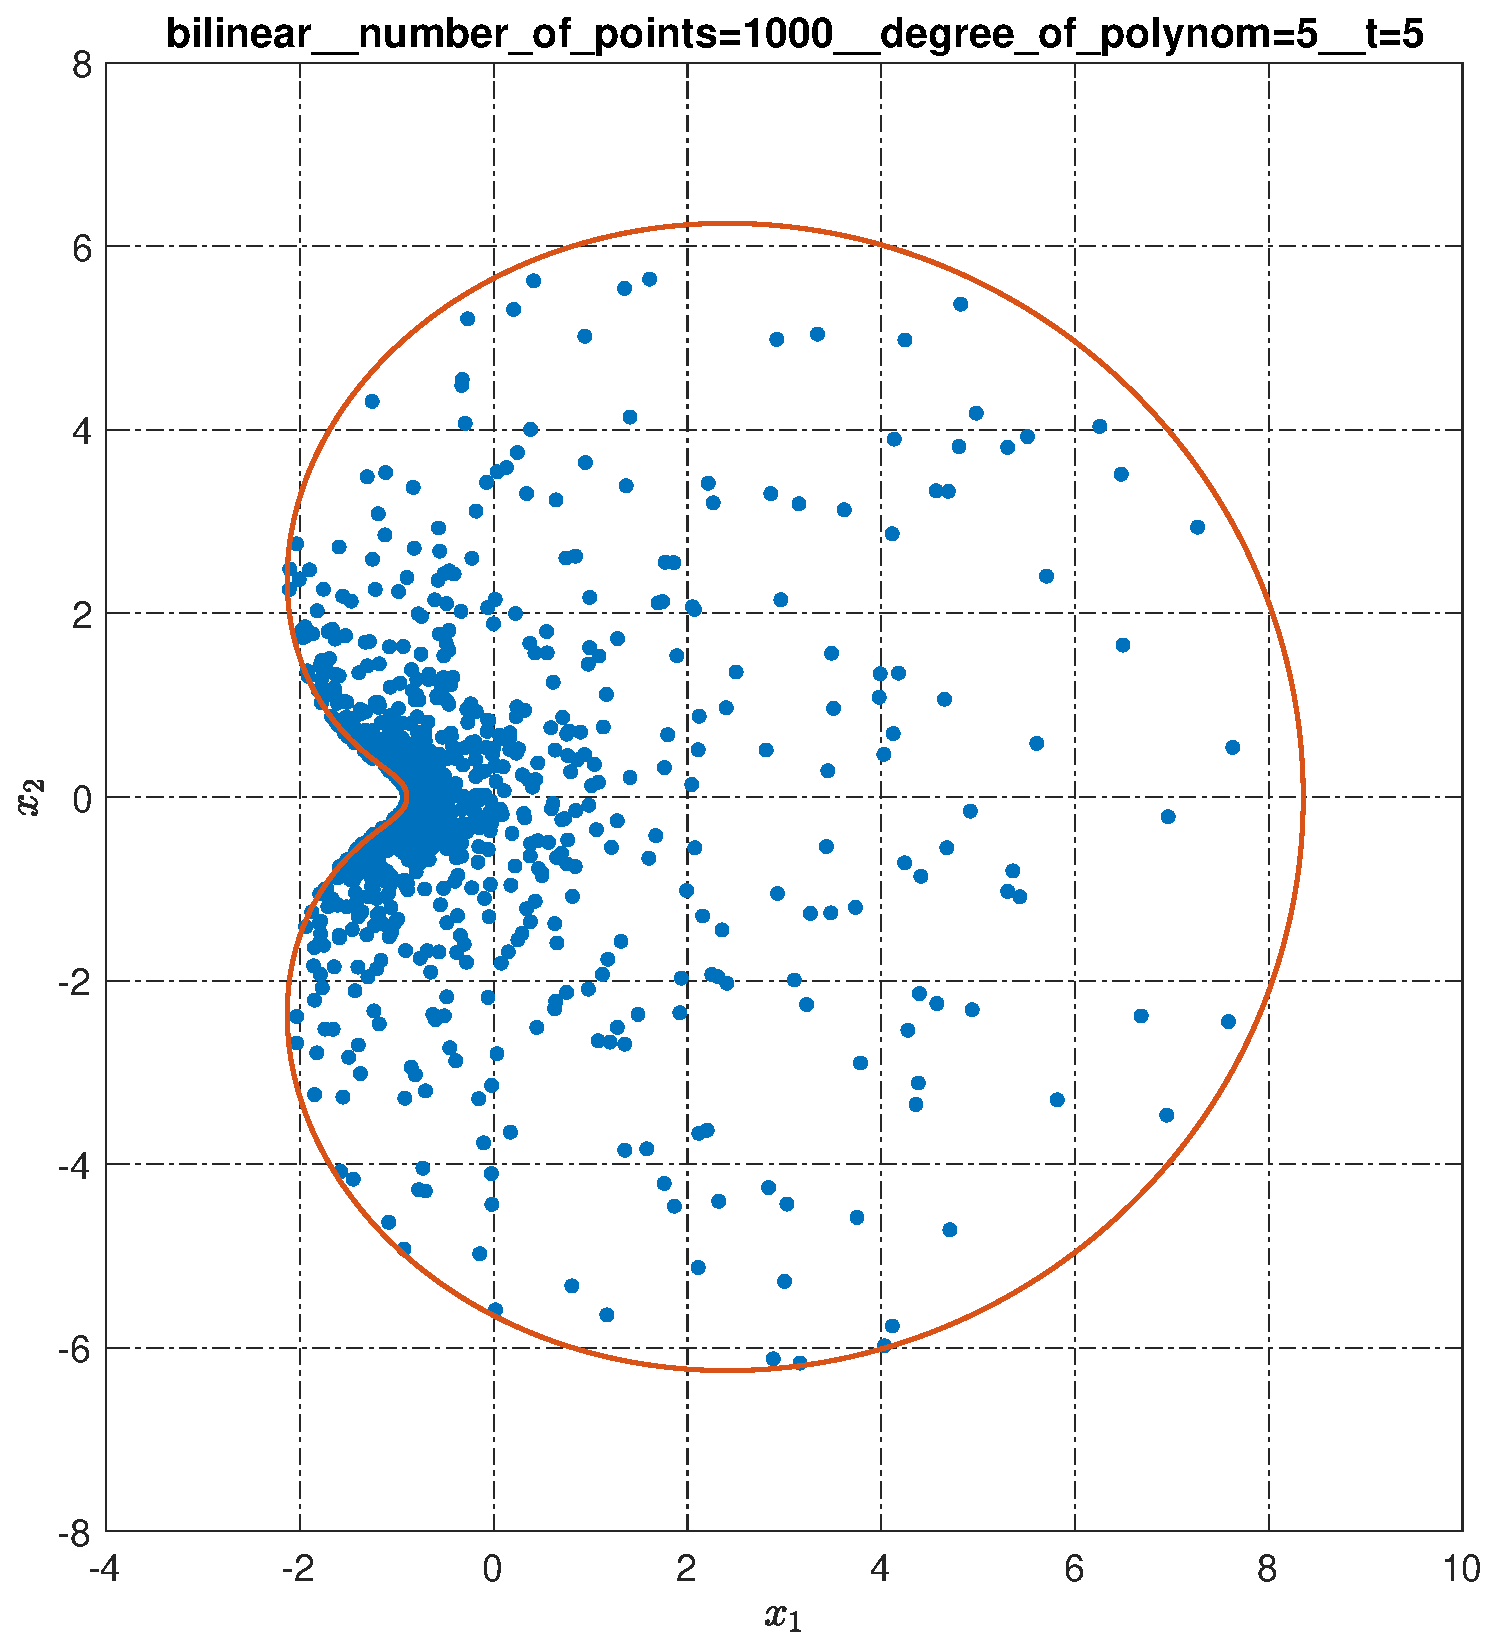
\includegraphics[width=\linewidth]{images/bilinear__number_of_points=1000__degree_of_polynom=5__t=5.eps}
 		\subcaption{$ N = 10^3 $, $k = 5 $, $T = 5 $ } 
 	\end{minipage}
 	\hfill
 	\begin{minipage}[b]{.3\linewidth} 
 		\small
 		\centering
 		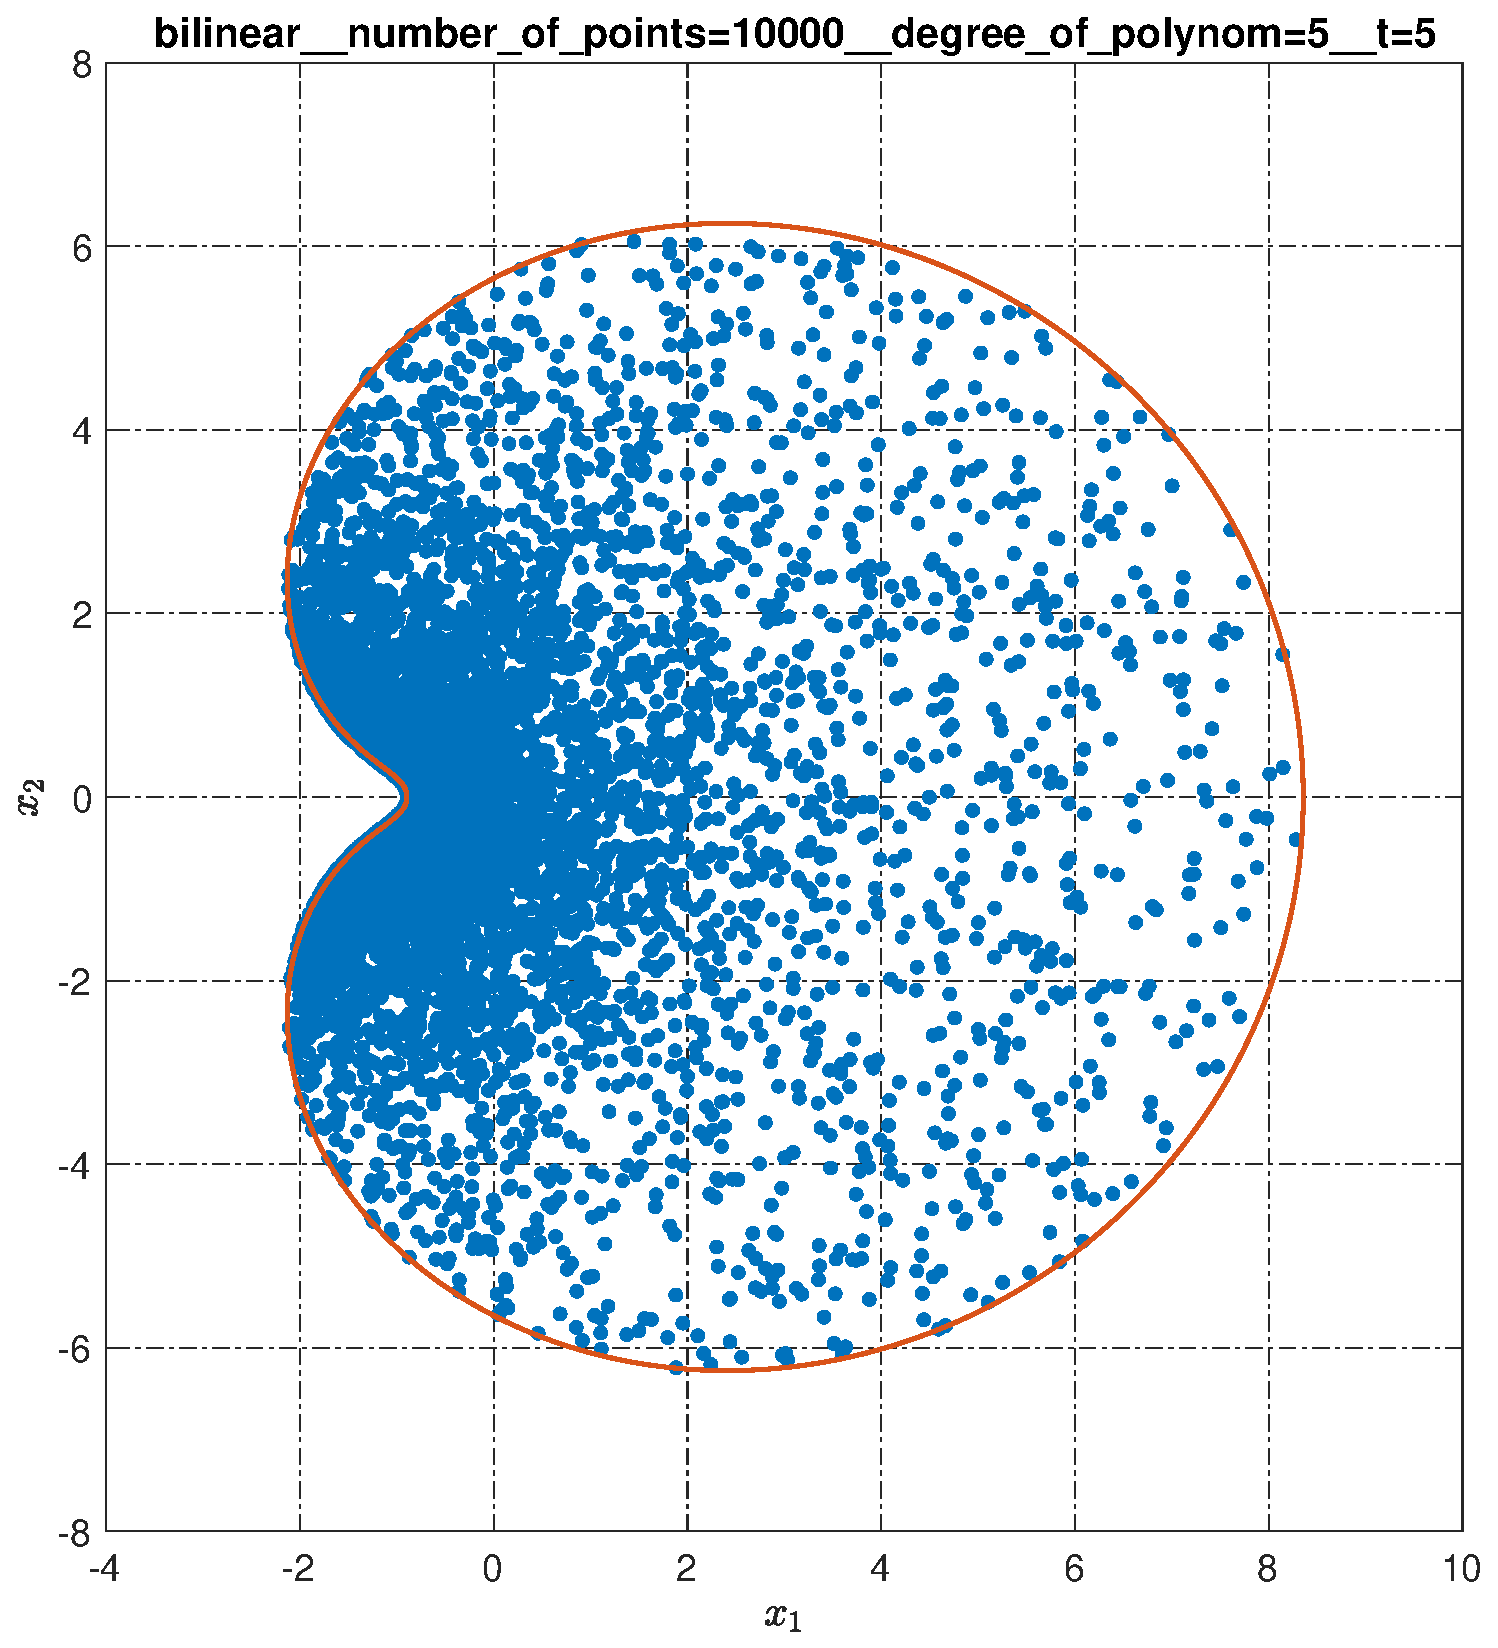
\includegraphics[width=\linewidth]{images/bilinear__number_of_points=10000__degree_of_polynom=5__t=5.eps}
 		\subcaption{$ N = 10^4 $, $k = 5 $, $T = 5 $ } 
 	\end{minipage} 
 	\hfill
 	\begin{minipage}[b]{.3\linewidth} 
 		\small
 		\centering 
 		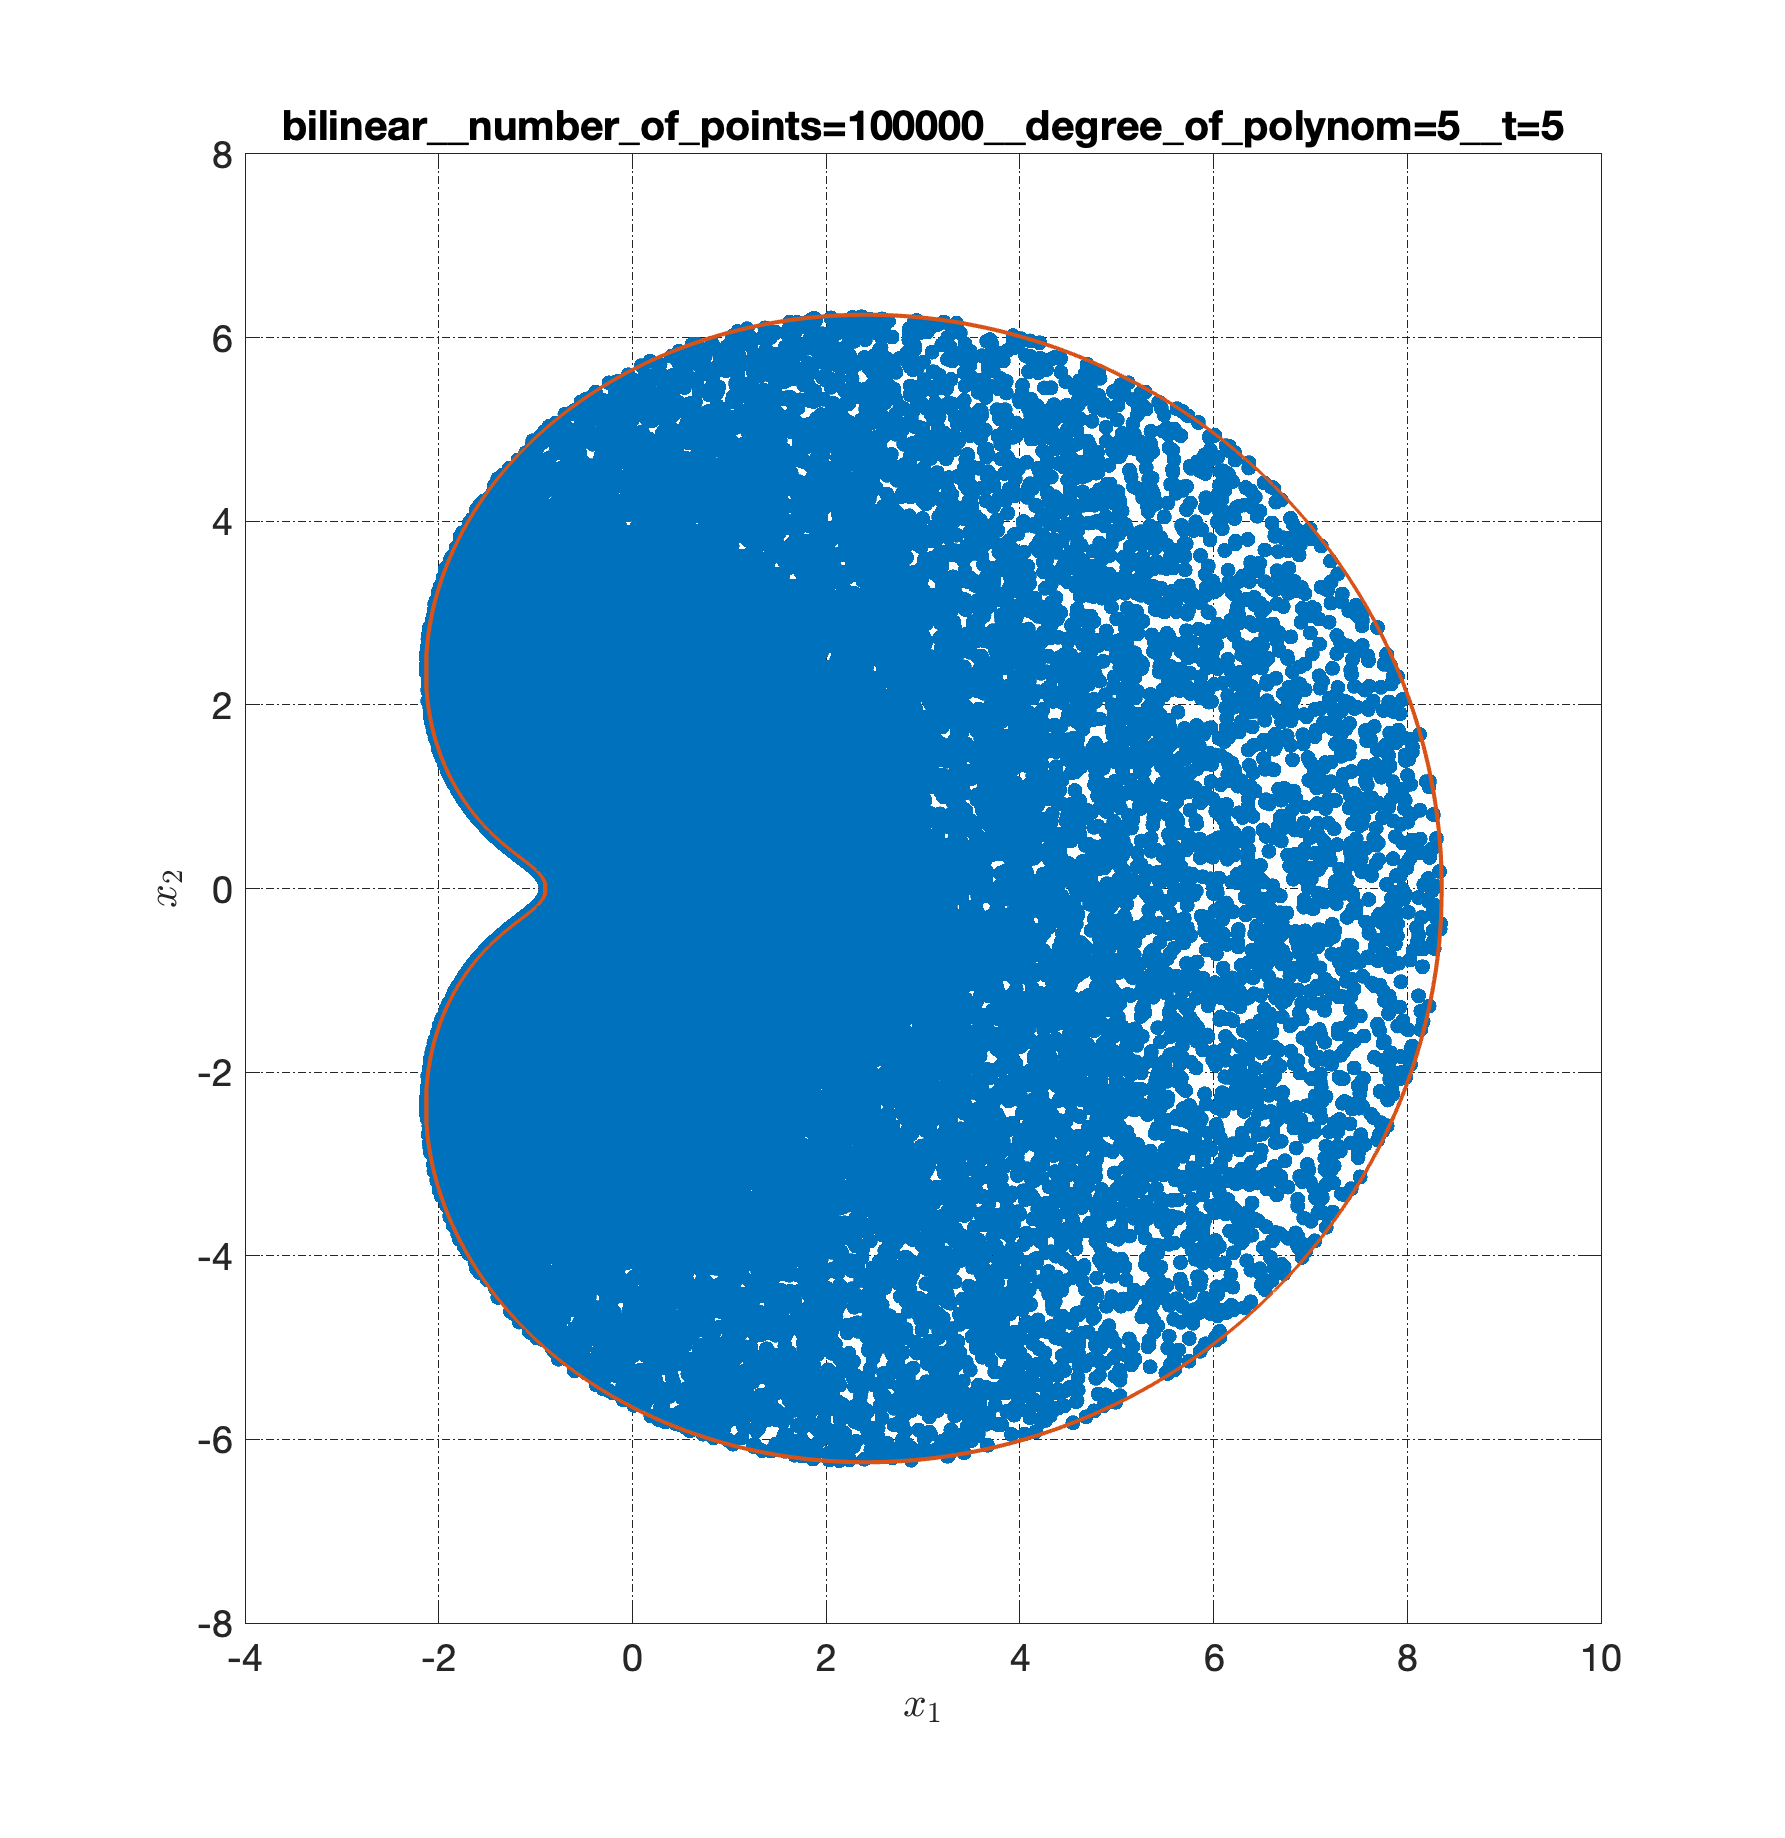
\includegraphics[width=\linewidth]{images/bilinear__number_of_points=100000__degree_of_polynom=5__t=5.eps}
 		\subcaption{$ N = 10^5 $, $k = 5 $, $T = 5 $ } 
 	\end{minipage}
 	\vfill
 	\hspace{-2.5ex}
 	\begin{minipage}[b]{.3\linewidth} 
 		\small
 		\centering
 		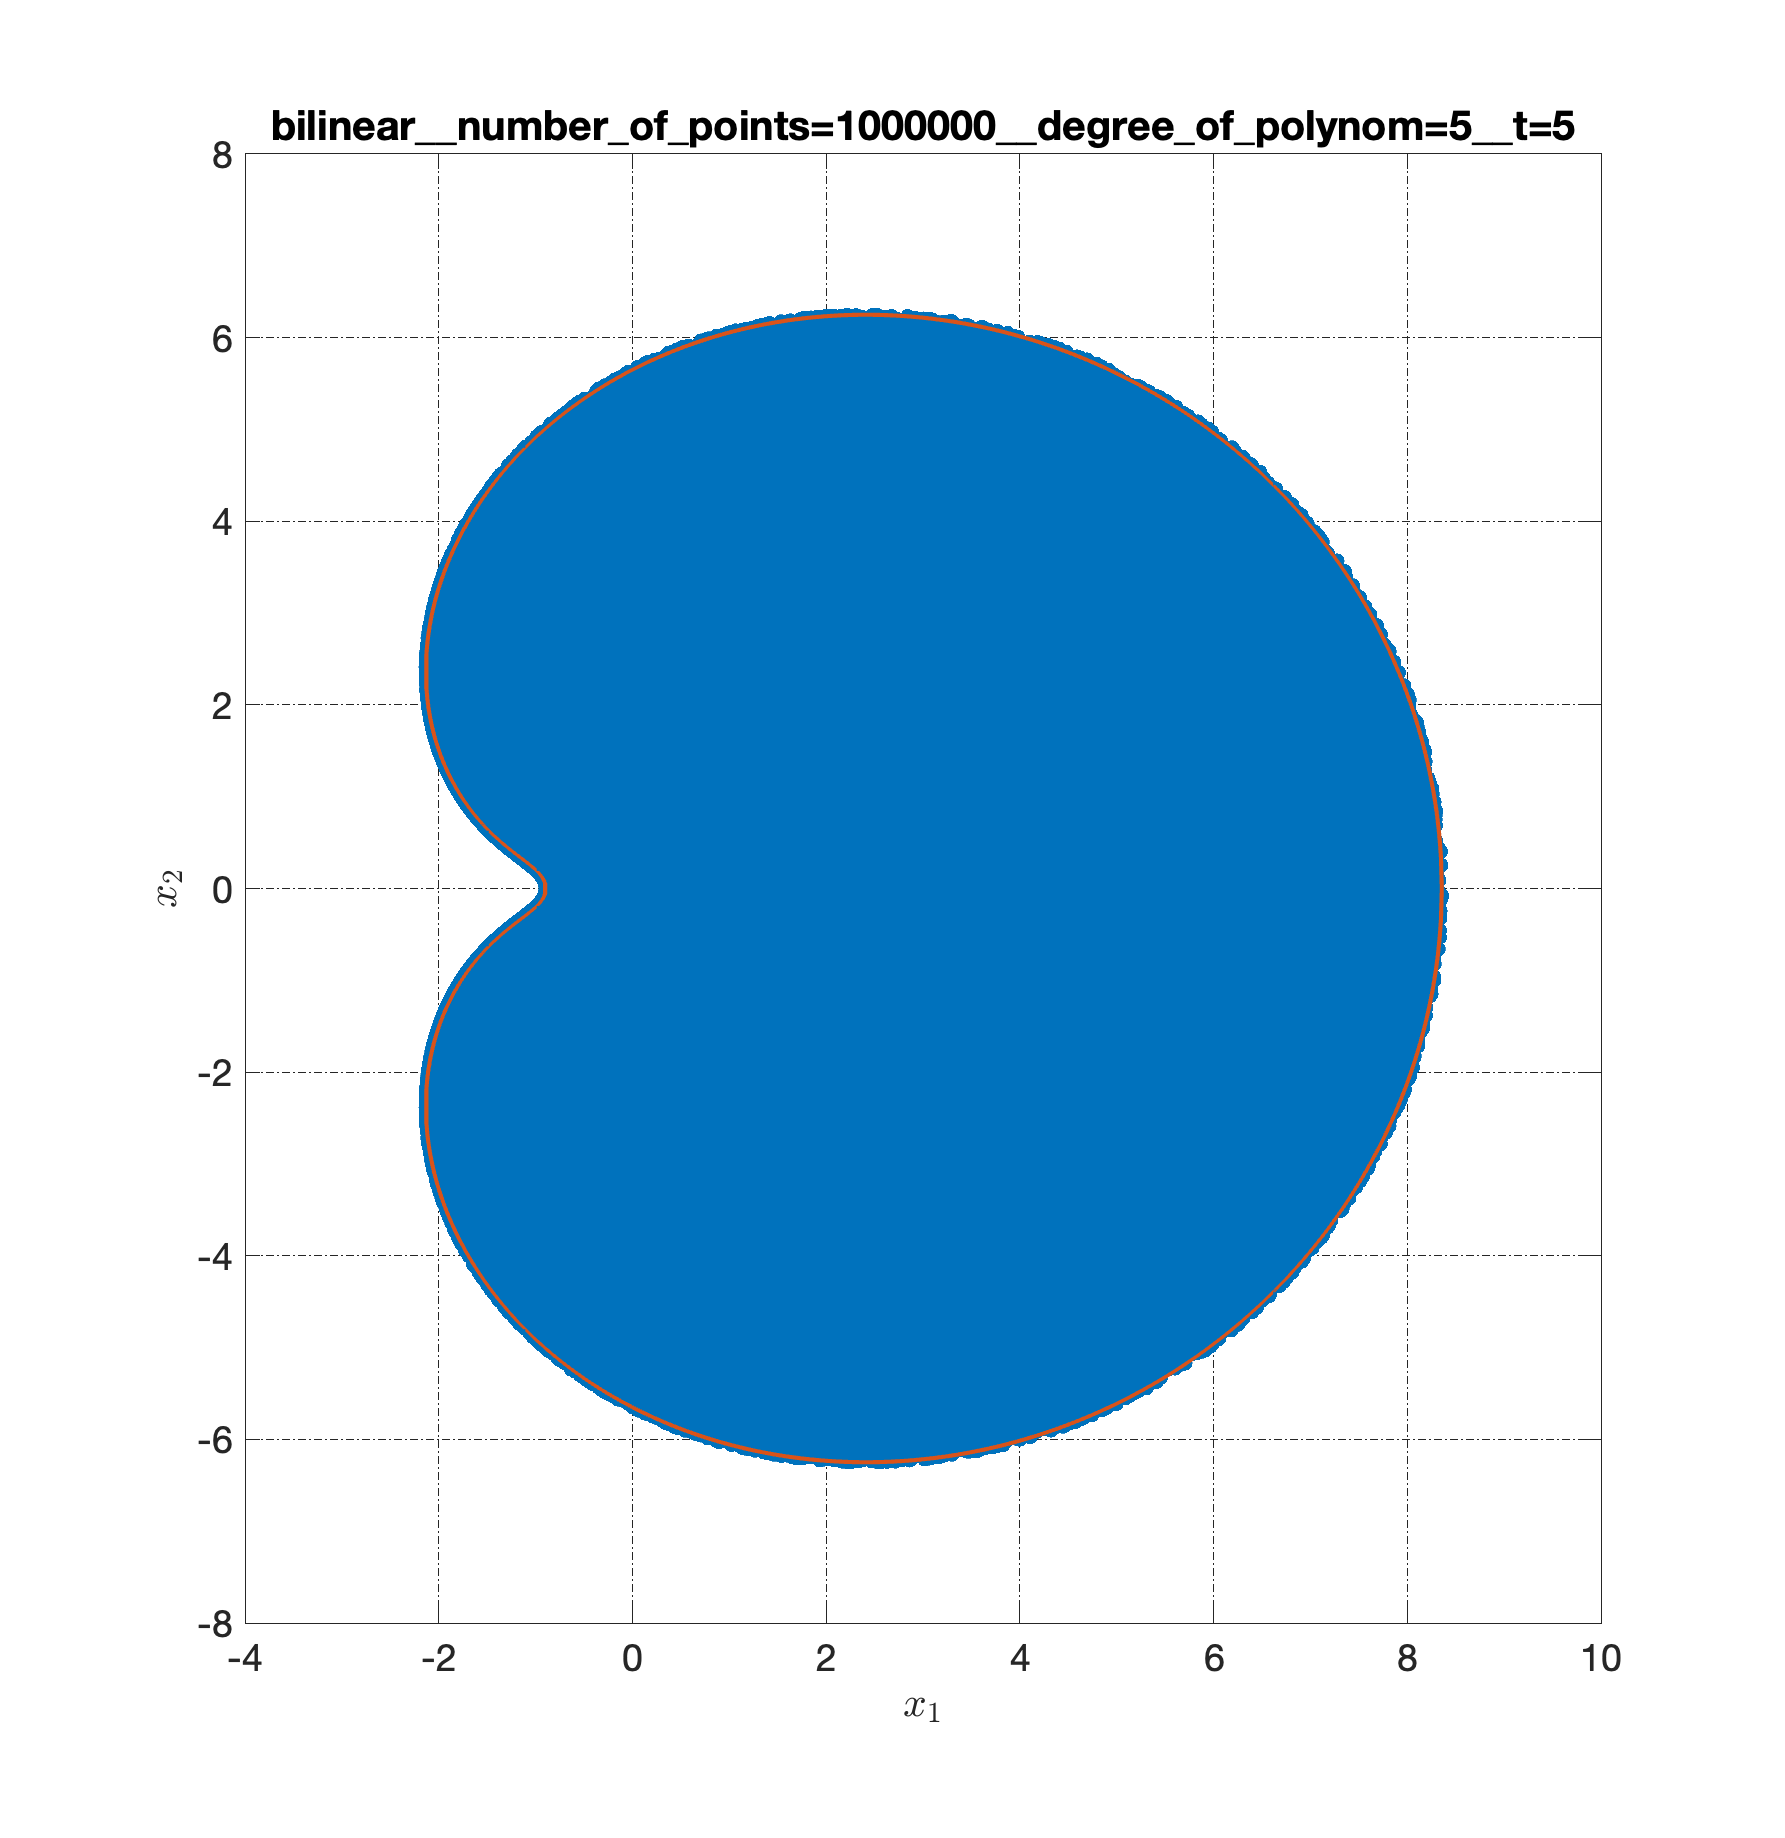
\includegraphics[width=\linewidth]{images/bilinear__number_of_points=1000000__degree_of_polynom=5__t=5.eps}
 		\subcaption{$ N = 10^6 $, $k = 5 $, $T = 5$} 
 	\end{minipage} 
 	\hfill
 	\begin{minipage}[b]{.3\linewidth} 
 		\small
 		\centering 
 		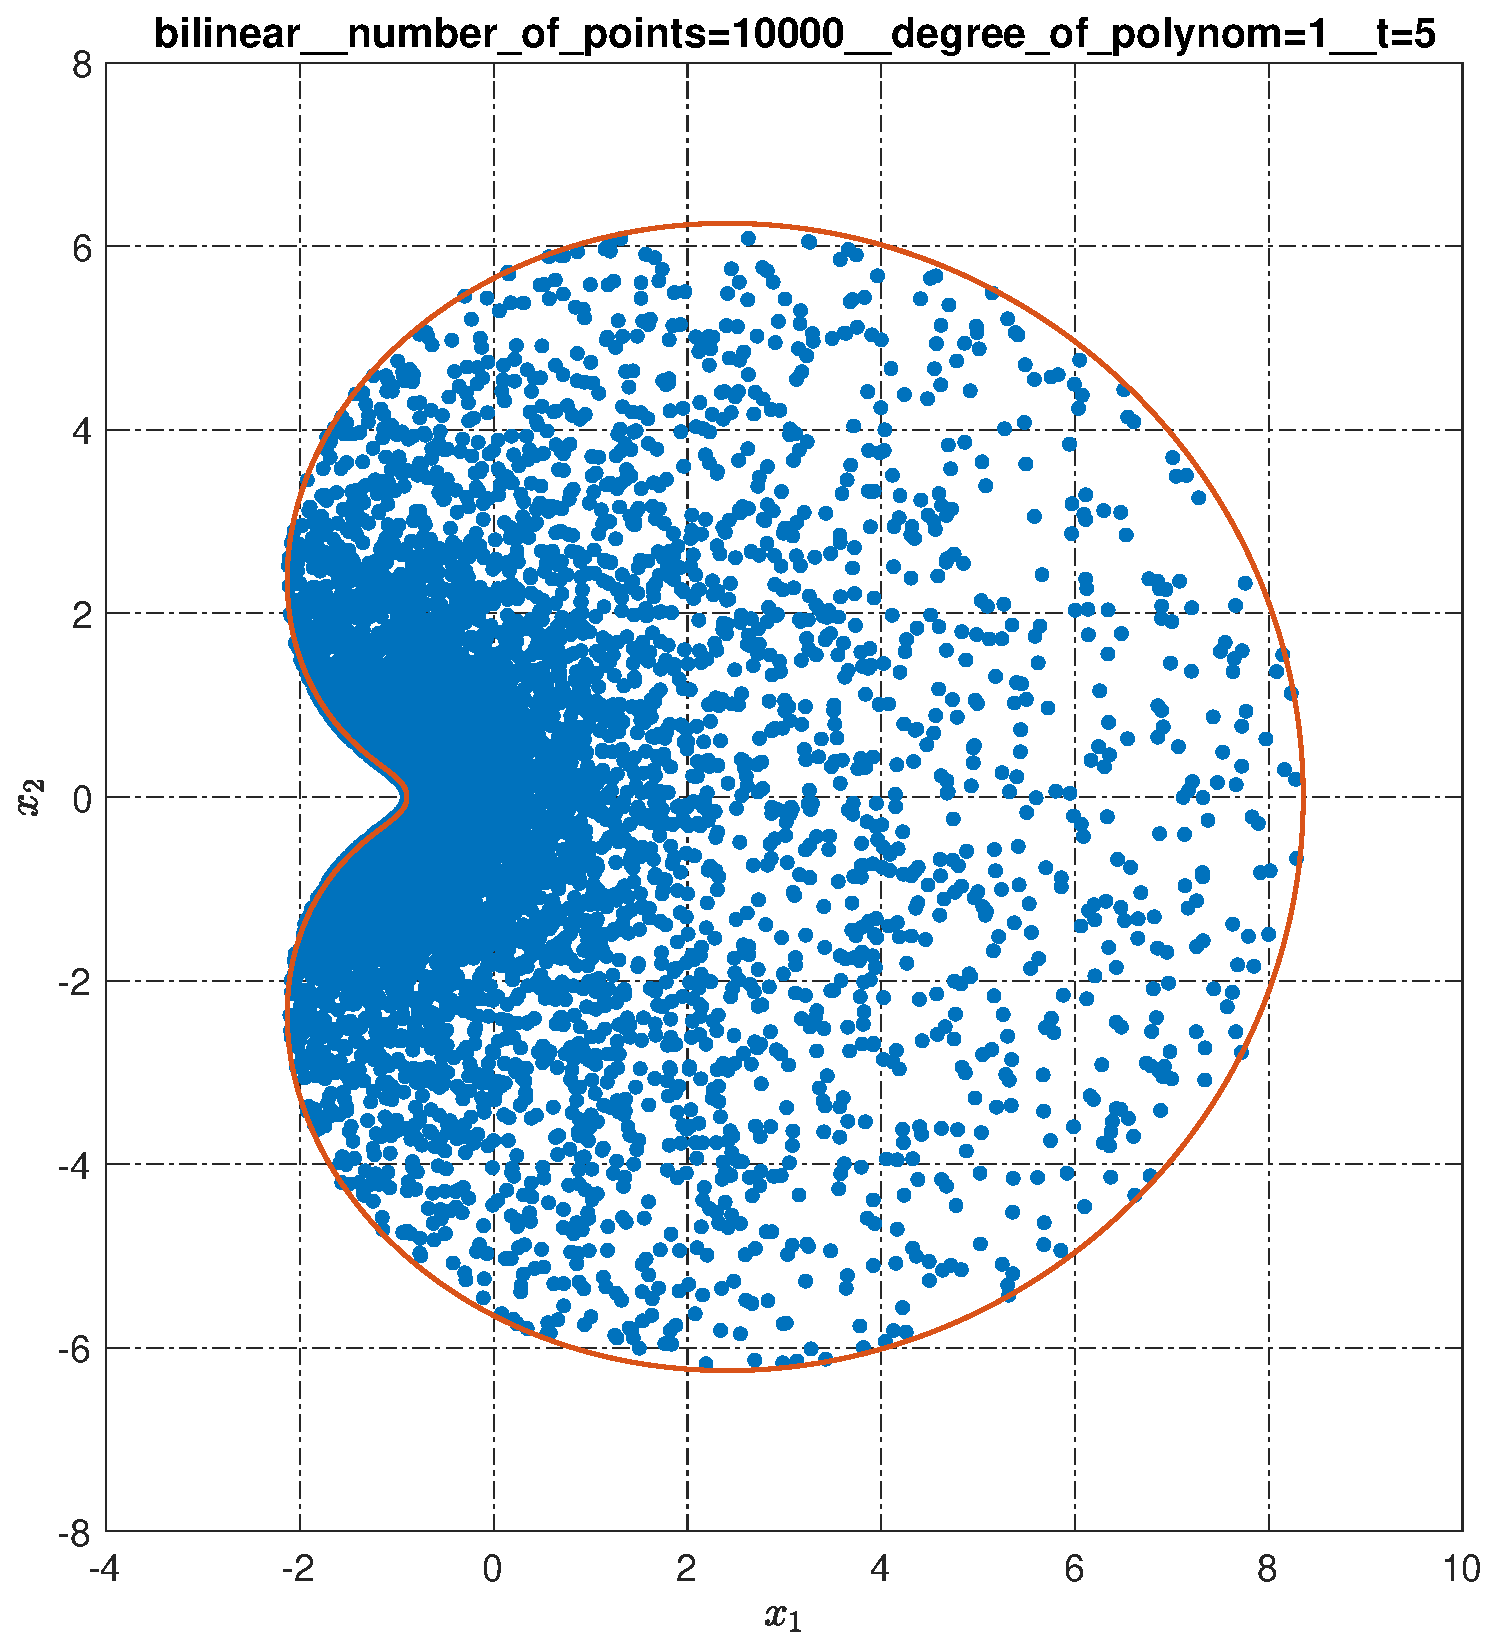
\includegraphics[width=\linewidth]{images/bilinear__number_of_points=10000__degree_of_polynom=1__t=5.eps}
 		\subcaption{$ N = 10^4 $, $k = 1 $, $T = 5 $} 
 	\end{minipage}
 	\hfill
 	\begin{minipage}[b]{.3\linewidth} 
 		\small
 		\centering
 		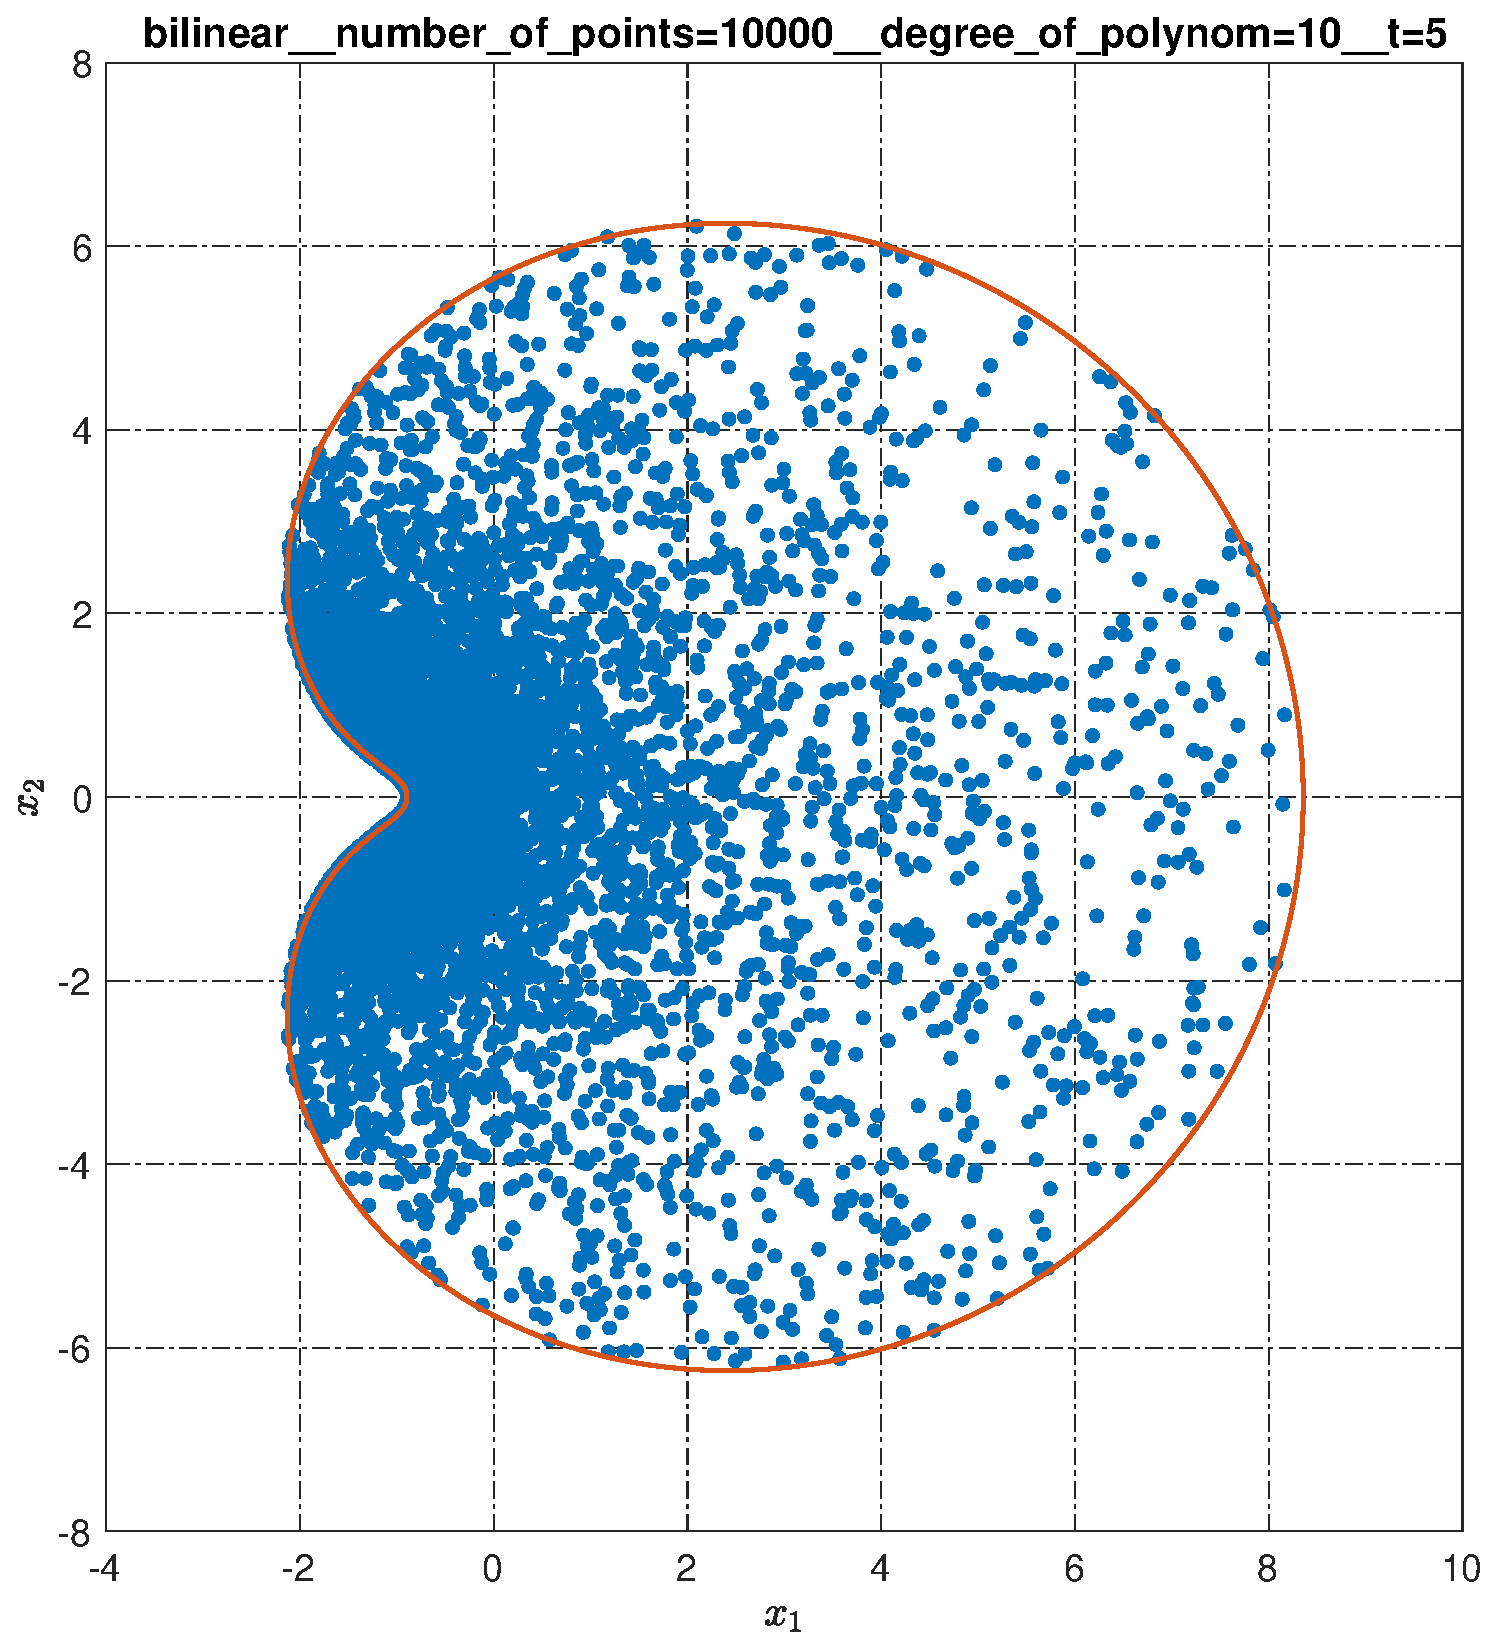
\includegraphics[width=\linewidth]{images/bilinear__number_of_points=10000__degree_of_polynom=10__t=5.eps}
 		\subcaption{$ N = 10^4 $, $k = 10 $, $T = 5 $} 
 	\end{minipage} 
 	\vfill
 	\hspace{-2.5ex}
 	\begin{minipage}[b]{.3\linewidth} 
 		\small
 		\centering 
 		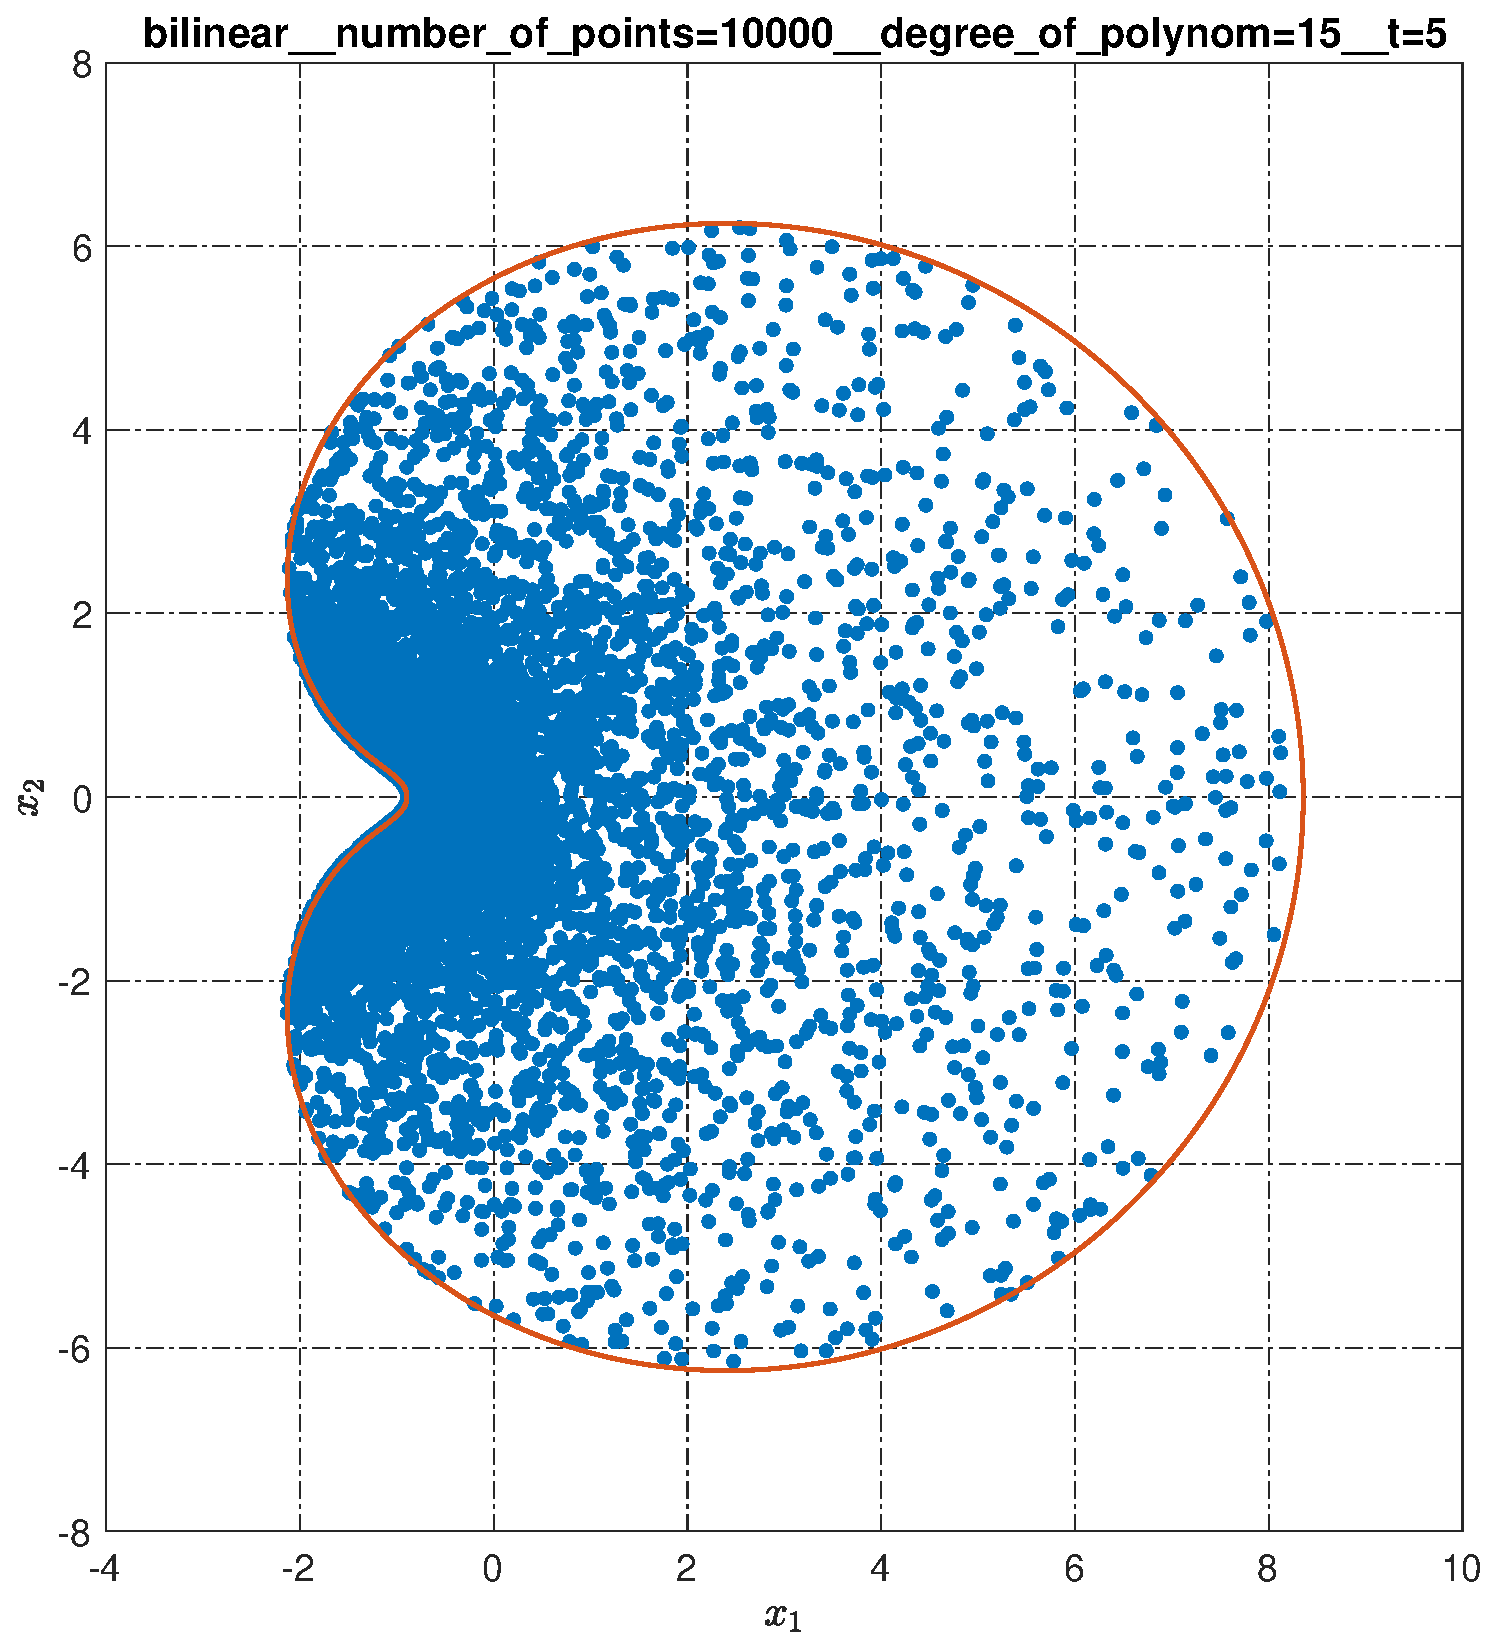
\includegraphics[width=\linewidth]{images/bilinear__number_of_points=10000__degree_of_polynom=15__t=5.eps}
 		\subcaption{$ N = 10^4 $, $k = 15 $, $T = 5 $ } 
 	\end{minipage}
 	\hfill
 	\begin{minipage}[b]{.3\linewidth} 
 		\small
 		\centering
 		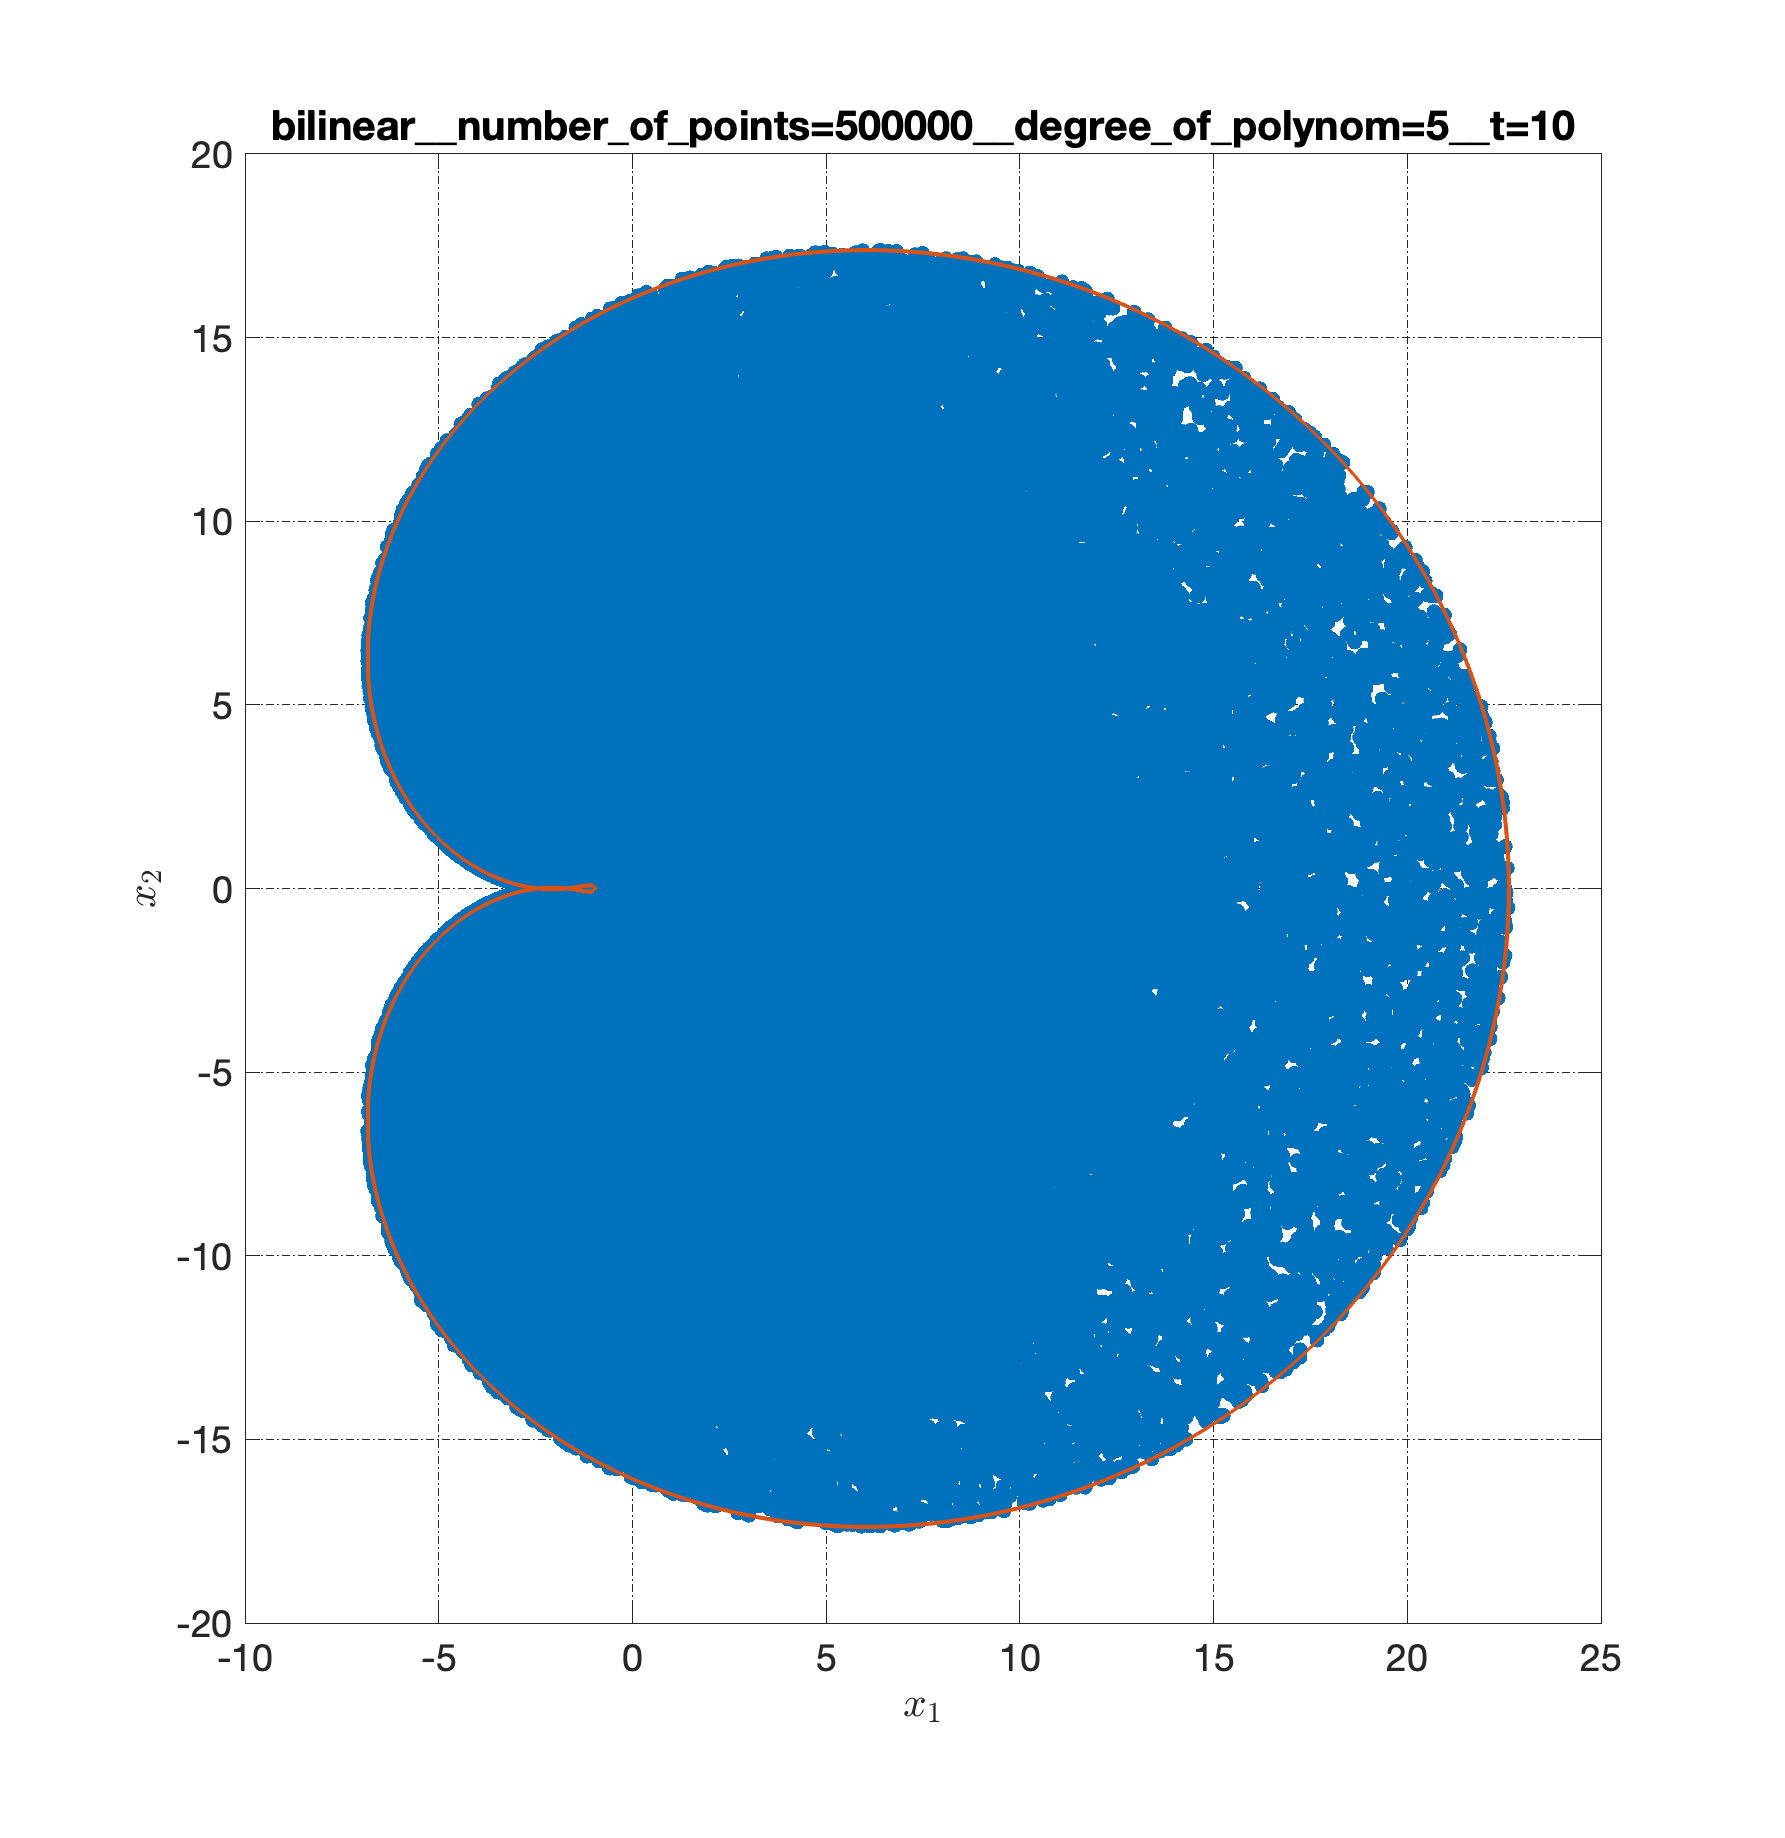
\includegraphics[width=\linewidth]{images/bilinear__number_of_points=500000__degree_of_polynom=5__t=10.eps}
 		\subcaption{$ N = 5\cdot10^5 $, $k = 5 $, $T = 10 $} 
 	\end{minipage} 
 	\hfill
 	\begin{minipage}[b]{.3\linewidth} 
 		\small
 		\centering
 		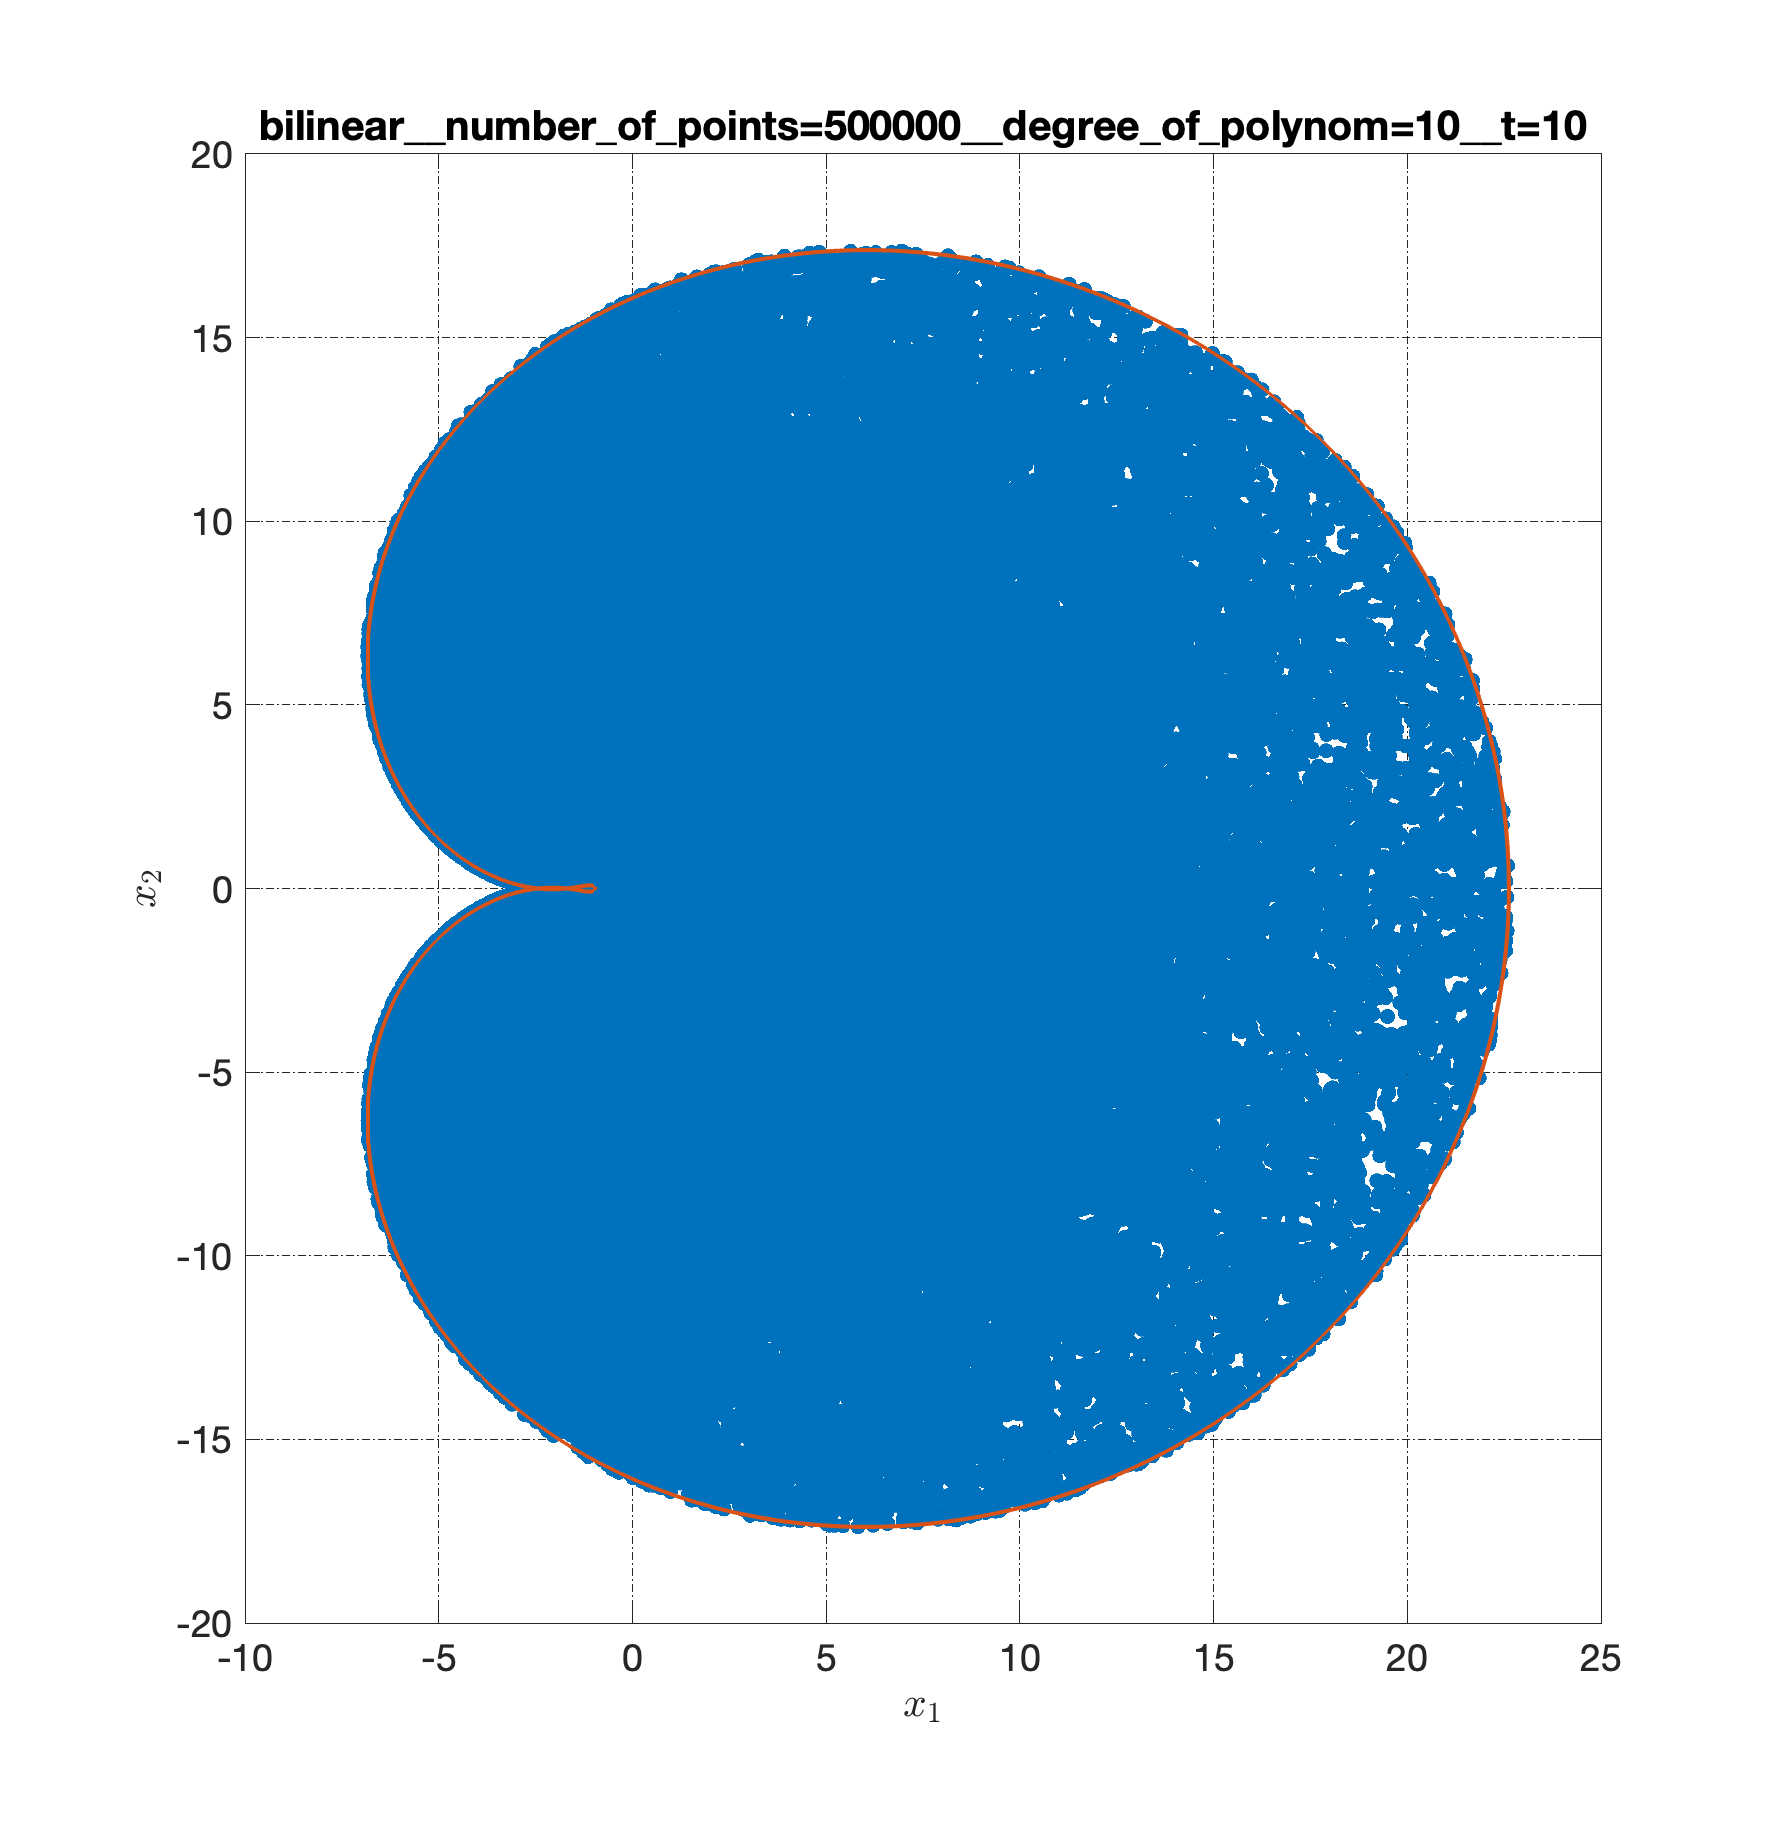
\includegraphics[width=\linewidth]{images/bilinear__number_of_points=500000__degree_of_polynom=10__t=10.eps}
 		\subcaption{$ N = 5\cdot10^5 $, $k = 10 $, $T = 10 $} 
 	\end{minipage} 
 	\caption{Результаты численного эксперимента для системы \eqref{ap:nonlinear_system1}.}\label{fig:ap:rs_nonlinear1}
 \end{figure}
 
 \textbf{Линейная система.} На интервале времени $ 0 \leqslant t \leqslant 1$ рассмотрим линейную систему 
 \begin{gather}\label{ap:linear_system1}
 	\begin{pmatrix} 
 		\dot{x}_1 \\
 		\dot{x}_2 
 	\end{pmatrix} = 
 	\begin{pmatrix}
 		0 & 1 \\
 		-2 & -3
 	\end{pmatrix}
 	\begin{pmatrix} 
 		x_1 \\
 		x_2 
 	\end{pmatrix} +
 	\begin{pmatrix} 1 \\ 0
 	\end{pmatrix} u
 \end{gather}
 при нулевых начальных условиях $x_1(0) = x_2(0) = 0 $ и ограничениях на управление 
 \begin{gather*}
 	\int\limits_0^1 u^2dt \leqslant 1.
 \end{gather*}
 
 На рисунке \ref{fig:ap:rs_linear1} показаны множества достижимости системы \eqref{ap:linear_system1} при различных $N$, $k$ и $T$.
 Красная линия --- граница множества достижимости, вычисленного аналитически.
 Видно, что при увеличении количества точек $N$, они плотнее заполняют множество достижимости (Рис. \ref{fig:ap:linearN103k5T1} --- \ref{fig:ap:linearN106k5T1}). 
 Также можно заметить, что при использовании линейных полиномов (при $k = 1$) точки лежат на эллипсоиде, близком к границе множества достижимости (Рис. \ref{fig:ap:linearN104k1T1}). 
 Этот эффект будет обсужден ниже.
 
 \textbf{Линейный осциллятор.} На интервале времени $ 0 \leqslant t \leqslant T$ рассмотрим линейную систему 
 \begin{gather}\label{ap:linear_oscil1}
 	\begin{pmatrix} 
 		\dot{x}_1 \\
 		\dot{x}_2 
 	\end{pmatrix} = 
 	\begin{pmatrix}
 		0 & 1 \\
 		-1 & 0
 	\end{pmatrix}
 	\begin{pmatrix} 
 		x_1 \\
 		x_2 
 	\end{pmatrix} +
 	\begin{pmatrix} 0 \\ 1
 	\end{pmatrix} u
 \end{gather}
 при нулевых начальных условиях $x_1(0) = x_2(0) = 0 $ и ограничениях на управление 
 \begin{gather*}
 	\int\limits_0^T u^2dt \leqslant 1.
 \end{gather*}
 
 На рисунке \ref{fig:ap:rs_linear_oscil} показаны множества достижимости системы \eqref{ap:linear_oscil1} при различных $N$, $k$ и $T$.
 Красная линия --- граница множества достижимости, вычисленного аналитически.
 Видно, что при увеличении количества точек, они плотнее заполняют множество достижимости.
 Как и в предыдущем примере, видно, что при использовании линейных полиномов на малом промежутке времени, $t = 1$ точки лежат на эллипсе, близком к границе множества достижимости (Рис. \ref{fig:ap:oscilN5103k1T1}, \ref{fig:ap:oscilN5104k1T1}), однако, при использовании таких же полиномов на интервале $t = 2\pi$ точки лежат на одном отрезке, который находится внутри множества достижимости (Рис. \ref{fig:ap:oscilN5103k1T2pi}, \ref{fig:ap:oscilN5104k1T2pi}). 
 Также можно заметить, что даже при большом количестве точек на интервале $t = 2\pi$ и $t = 4\pi$, они не покрывают все множество достижимости, особенно рядом с границей (Рис. \ref{fig:ap:oscilN5103k5T2pi}, \ref{fig:ap:oscilN5104k5T2pi}, \ref{fig:ap:oscilN5104k5T4pi}). 
 Это можно объяснить тем, что управления, которые ведут на границу множества достижимости системы \eqref{ap:linear_oscil1} являются периодическими функциями, и плохо аппроксимируются  алгебраическими полиномами небольшого порядка, которые были использованы в алгоритме.
 
 \textbf{Нелинейная система.} В следующем примере рассмотрим нелинейную систему 
 \begin{gather}\label{ap:nonlinear_system1}
 	\begin{gathered}
 	\dot{x}_1 = x_2 u_1 - (1 + x_1) u_2,\\
 	\dot{x}_2 = -(1 + x_1) u_1 - x_2 u_2
 	\end{gathered}
 \end{gather}
 на интервале $ 0 \leqslant t \leqslant 5$.
 Начальное состояние $x_1(0) = x_2(0) = 0 $, а управление стеснено такими же ограничениями, что и в прошлом примере
 \begin{gather*}
 	\int\limits_0^1 u^2dt \leqslant 1.
 \end{gather*}
 
 На рисунке \ref{fig:ap:rs_nonlinear1} показаны множества достижимости системы \eqref{ap:nonlinear_system1} при различных $N$ и $k$.
 Красная линия --- граница множества достижимости, вычисленного аналитически.
 Видно, что при увеличении количества точек, они заполняют множество достижимости, однако, в отличие от линейной системы в предыдущем примере, здесь точки заполняют множество достижимости неравномерно.
 
 \begin{figure}[ht]
 	\centering
 	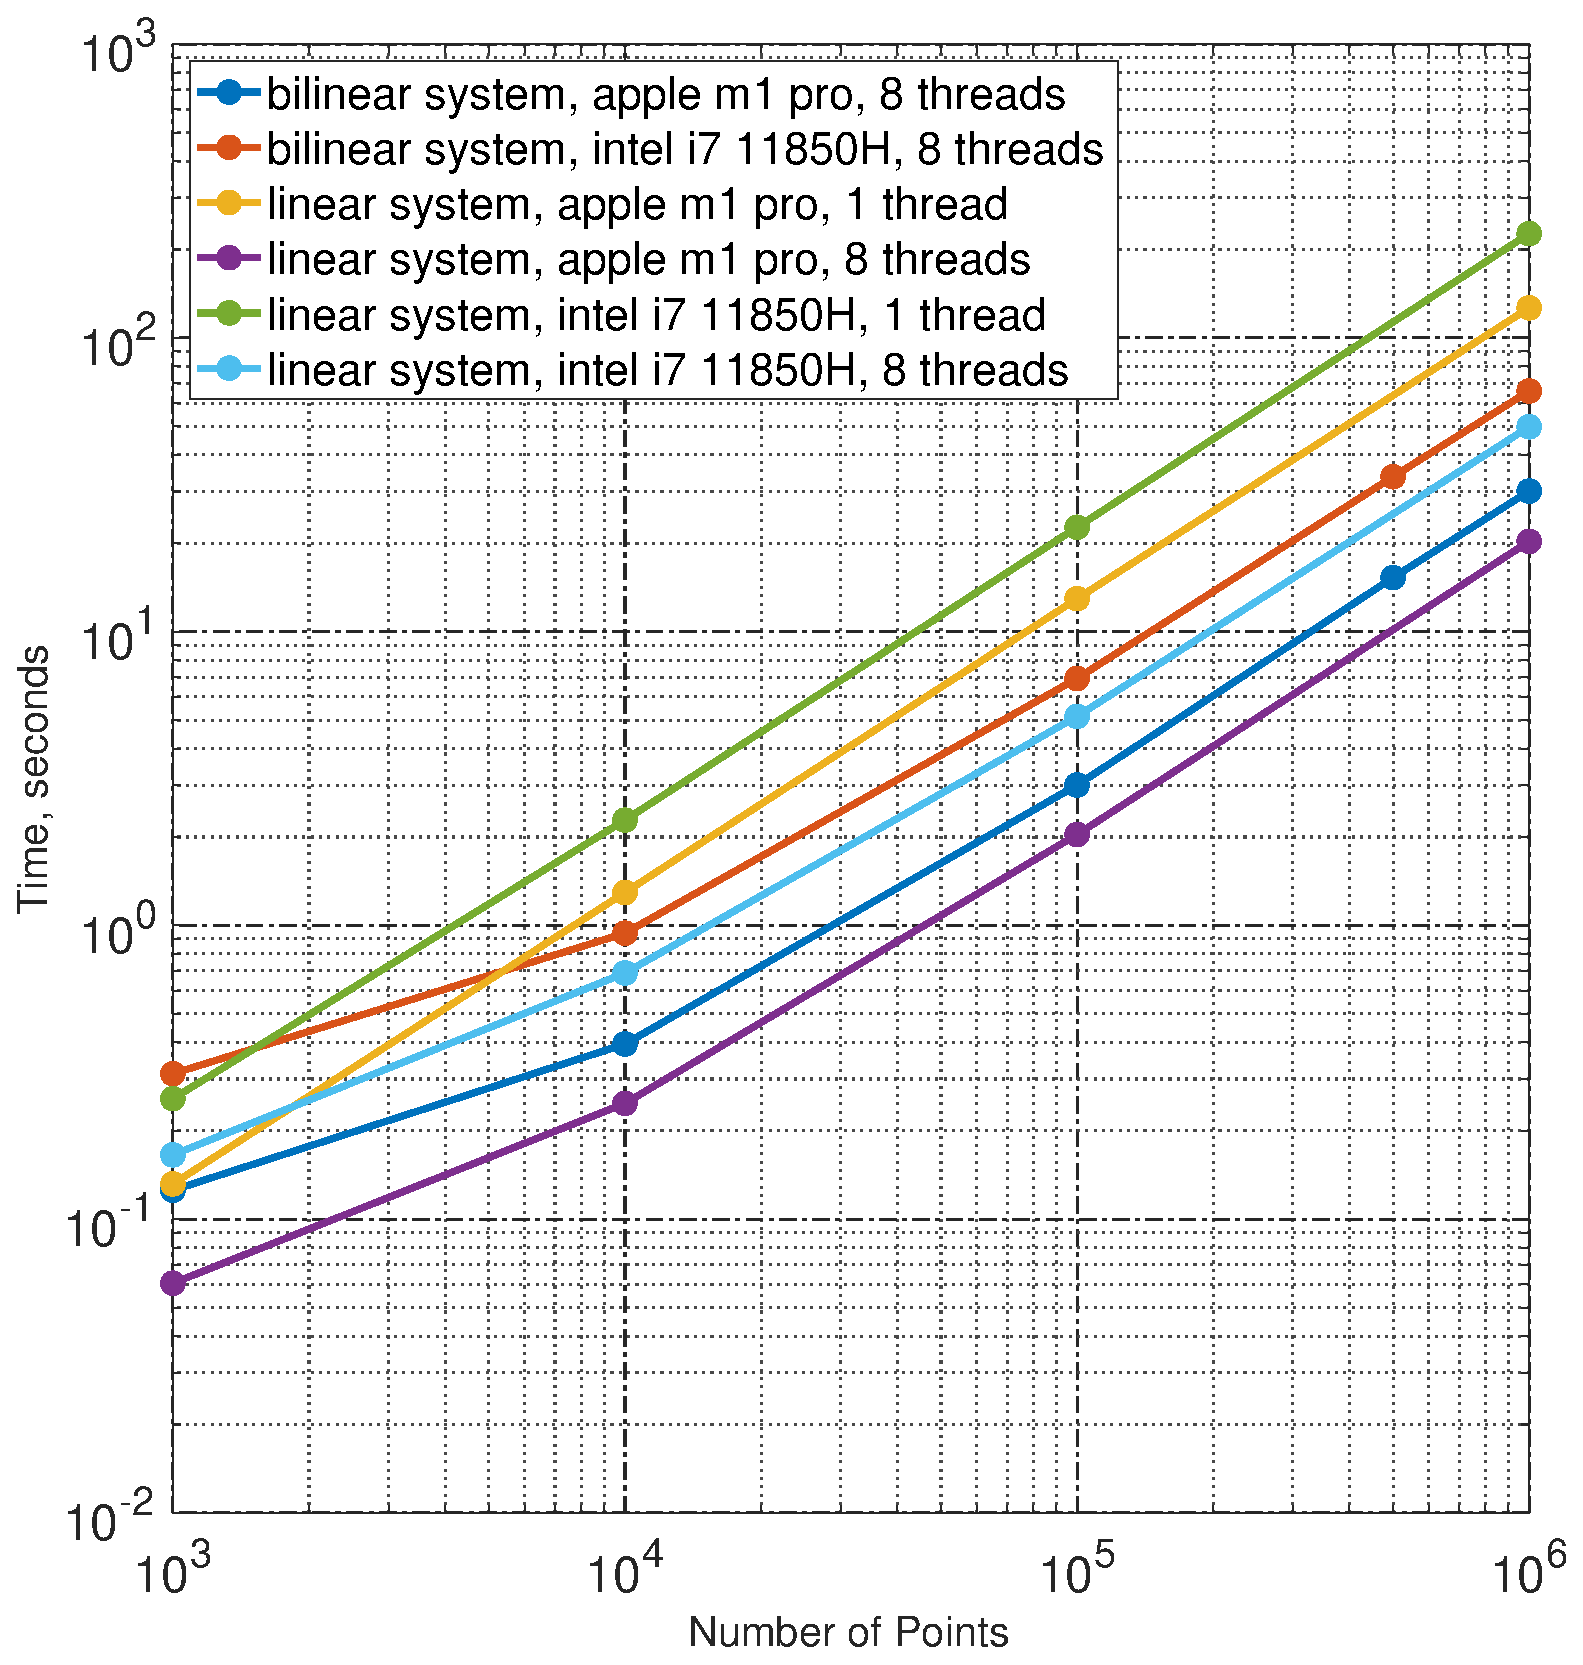
\includegraphics[width=0.5\textwidth]{images/time_complexity.eps}
 	\caption{Время работы алгоритма.}
 	\label{fig:ap:timings}
 \end{figure}

 Следующий рисунок, рисунок \ref{fig:ap:timings}, показывает зависимость времени работы алгоритма от количества точек и числа параллельных потоков (threads).
 Видно, что при параллельном вычислении точек множества достижимости время работы алгоритма существенно сокращается при постоянном количестве точек.

 \subsection{Влияние выбора коэффициентов }
 
 \begin{figure}[ht]
 	\centering
 	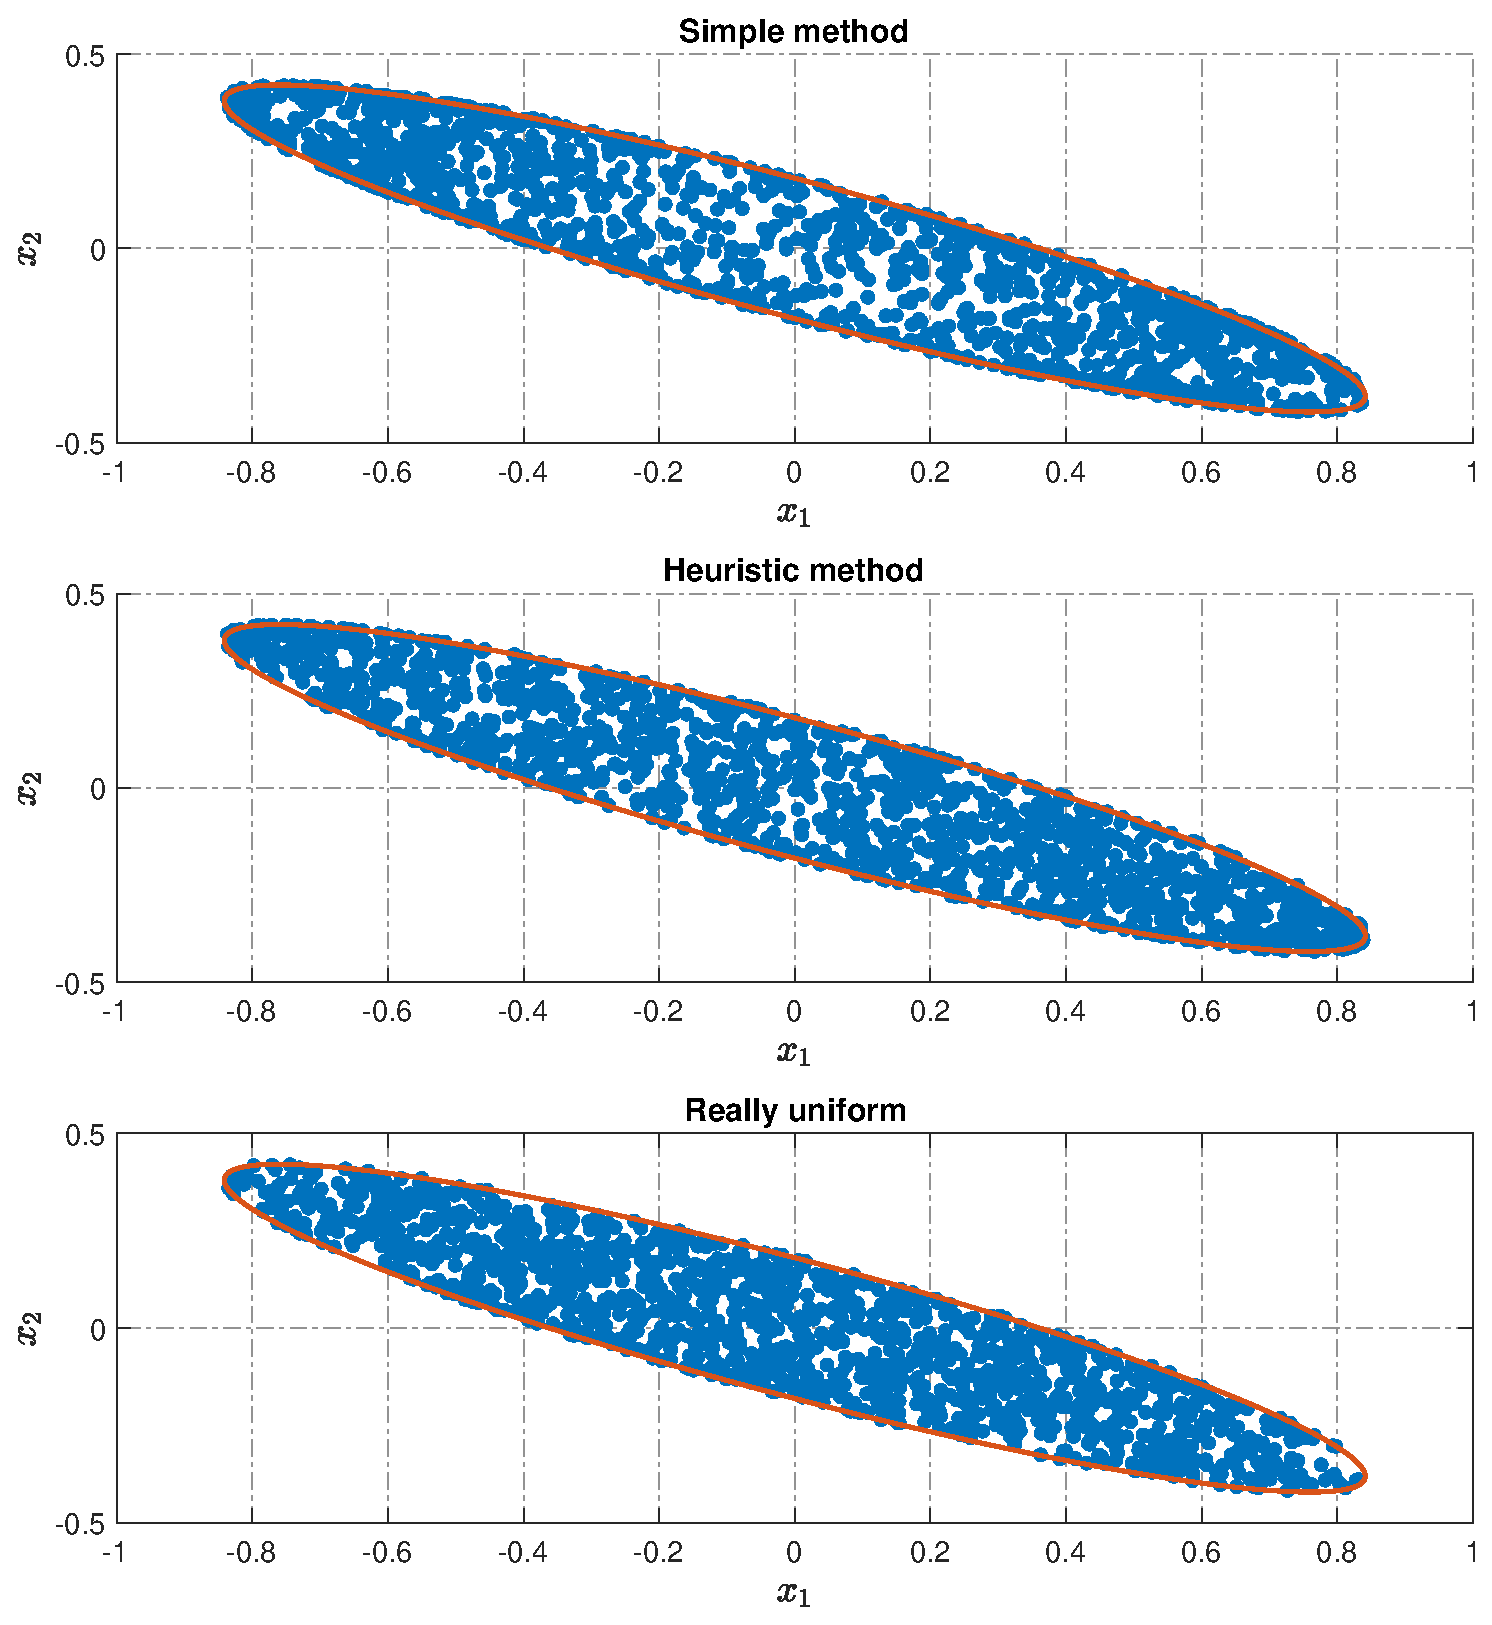
\includegraphics[width=0.6\textwidth]{images/three_linear_system_sets.eps}
 	\caption{Влияние выбора коэффициентов $C_i$.}
 	\label{fig:ap:coeffs_RS}
 \end{figure}
 
 Оказалось, что равномерность заполнения множеств достижимости точками сильно зависит от выбора коэффициентов $C_i$. 
 Автор использовал два метода получения случайной матрицы $C_i \in \mathbb{R}^{r \times k+1}$ с заданной фробениусовой нормой $ \|C_i\| = \mu$. 
 
 Первый метод состоит в генерации $r (k + 1)$ равномерно распределенных скаляров $ \overline{c}_{i, j}$, $ j = 1\dots r (k + 1)$ в диапазоне $[-1;1] $, $\overline{c}_{i, j} \sim \mathcal{U}[-1;1]$, составлении из них матрицы $\overline{C_i} \in \mathbb{R}^{r \times k+1}$ и нормировании ее
 \begin{gather*}
 		C_i = \frac{\mu}{\|C_i\|}\overline{C_i}.
 \end{gather*}
 
 В верхней части рисунка \ref{fig:ap:coeffs_RS} представлено множество достижимости системы \eqref{ap:linear_system1}, полученное с использованием этого метода генерации коэффициентов. 
 
 Второй метод также состоит из покомпонентной генерации равномерно распределенных скаляров, однако, диапазон, в котором происходит генерация уменьшается на сумму квадратов уже сгенерированных компонентов. 
 Так, нулевой компонент $c_{i, 0}$ равномерно распределен в диапазоне $[-\mu; \mu]$, $c_{i, 0} \sim \mathcal{U}[-\mu; \mu]$. 
 Первый компонент выбирается 
 \begin{gather*}
 	 c_{i, 1} \sim \mathcal{U}\left[-\sqrt{\mu^2 - c_{i, 0}^2}; \sqrt{\mu^2 - c_{i, 0}^2}\right].
 \end{gather*} 
 Аналогично выбираются все остальные компоненты, кроме последнего
 \begin{gather*}
 	c_{i, j} \sim \mathcal{U}\left[-\sqrt{\mu^2 - \sum\limits_{s = 0}^j c_{i, s}^2}; \sqrt{\mu^2 - \sum\limits_{s = 0}^j c_{i, s}^2}\right], \qquad 1 \leqslant j \leqslant r(k+1) - 2.
 \end{gather*} 
 Величина последнего коэффициента выбирается равной $\sqrt{\mu^2 - \sum\limits_{s = 0}^{r(k+1) - 2} c_{i, s}^2} $, а случайно выбирается лишь его знак.
 На рисунке \ref{fig:ap:coeffs_RS} приведено три результата генерации одинакового количества точек множества достижимости системы \eqref{ap:linear_system1}.
 На верхнем рисунке показан результат использования первого метода генерации коэффициентов, на среднем рисунке использован второй метод, а в нижней части рисунка аналитически рассчитанный эллипсоид множества достижимости равномерно заполнен таким же количеством точек, как и в первых двух частях рисунка. 
 Видно, что в верхней части рисунка эллипсоид заполнен менее равномерно, чем в средней и тем более, чем в нижней. 
 
 Для того, чтобы исследовать причины такого результата, решим обратную задачу, восстановив управления, ведущие в равномерно распределенные точки третьего рисунка и коэффициенты разложения этих управлений по той же системе полиномов третьего порядка, что и использовалась в первых двух рисунках.
 
 Точки множества достижимости, полученные в результате работы Алгоритма \ref{ap:method} можно представить в виде $x_i(T, u_i) = M C_i^{\top}$, где $M$ --- матрица, составленная из решений системы \eqref{ap:linear_system1}, порожденных управлениями в виде полиномов $p_k(t)$, 
 \begin{gather}\label{ap:matrix_M}
 	 M = \big(x(T, p_0), x(T, p_1), \dots, x(T, p_k)\big).
 \end{gather} 
 
 \begin{figure}[ht]
 	\centering
 	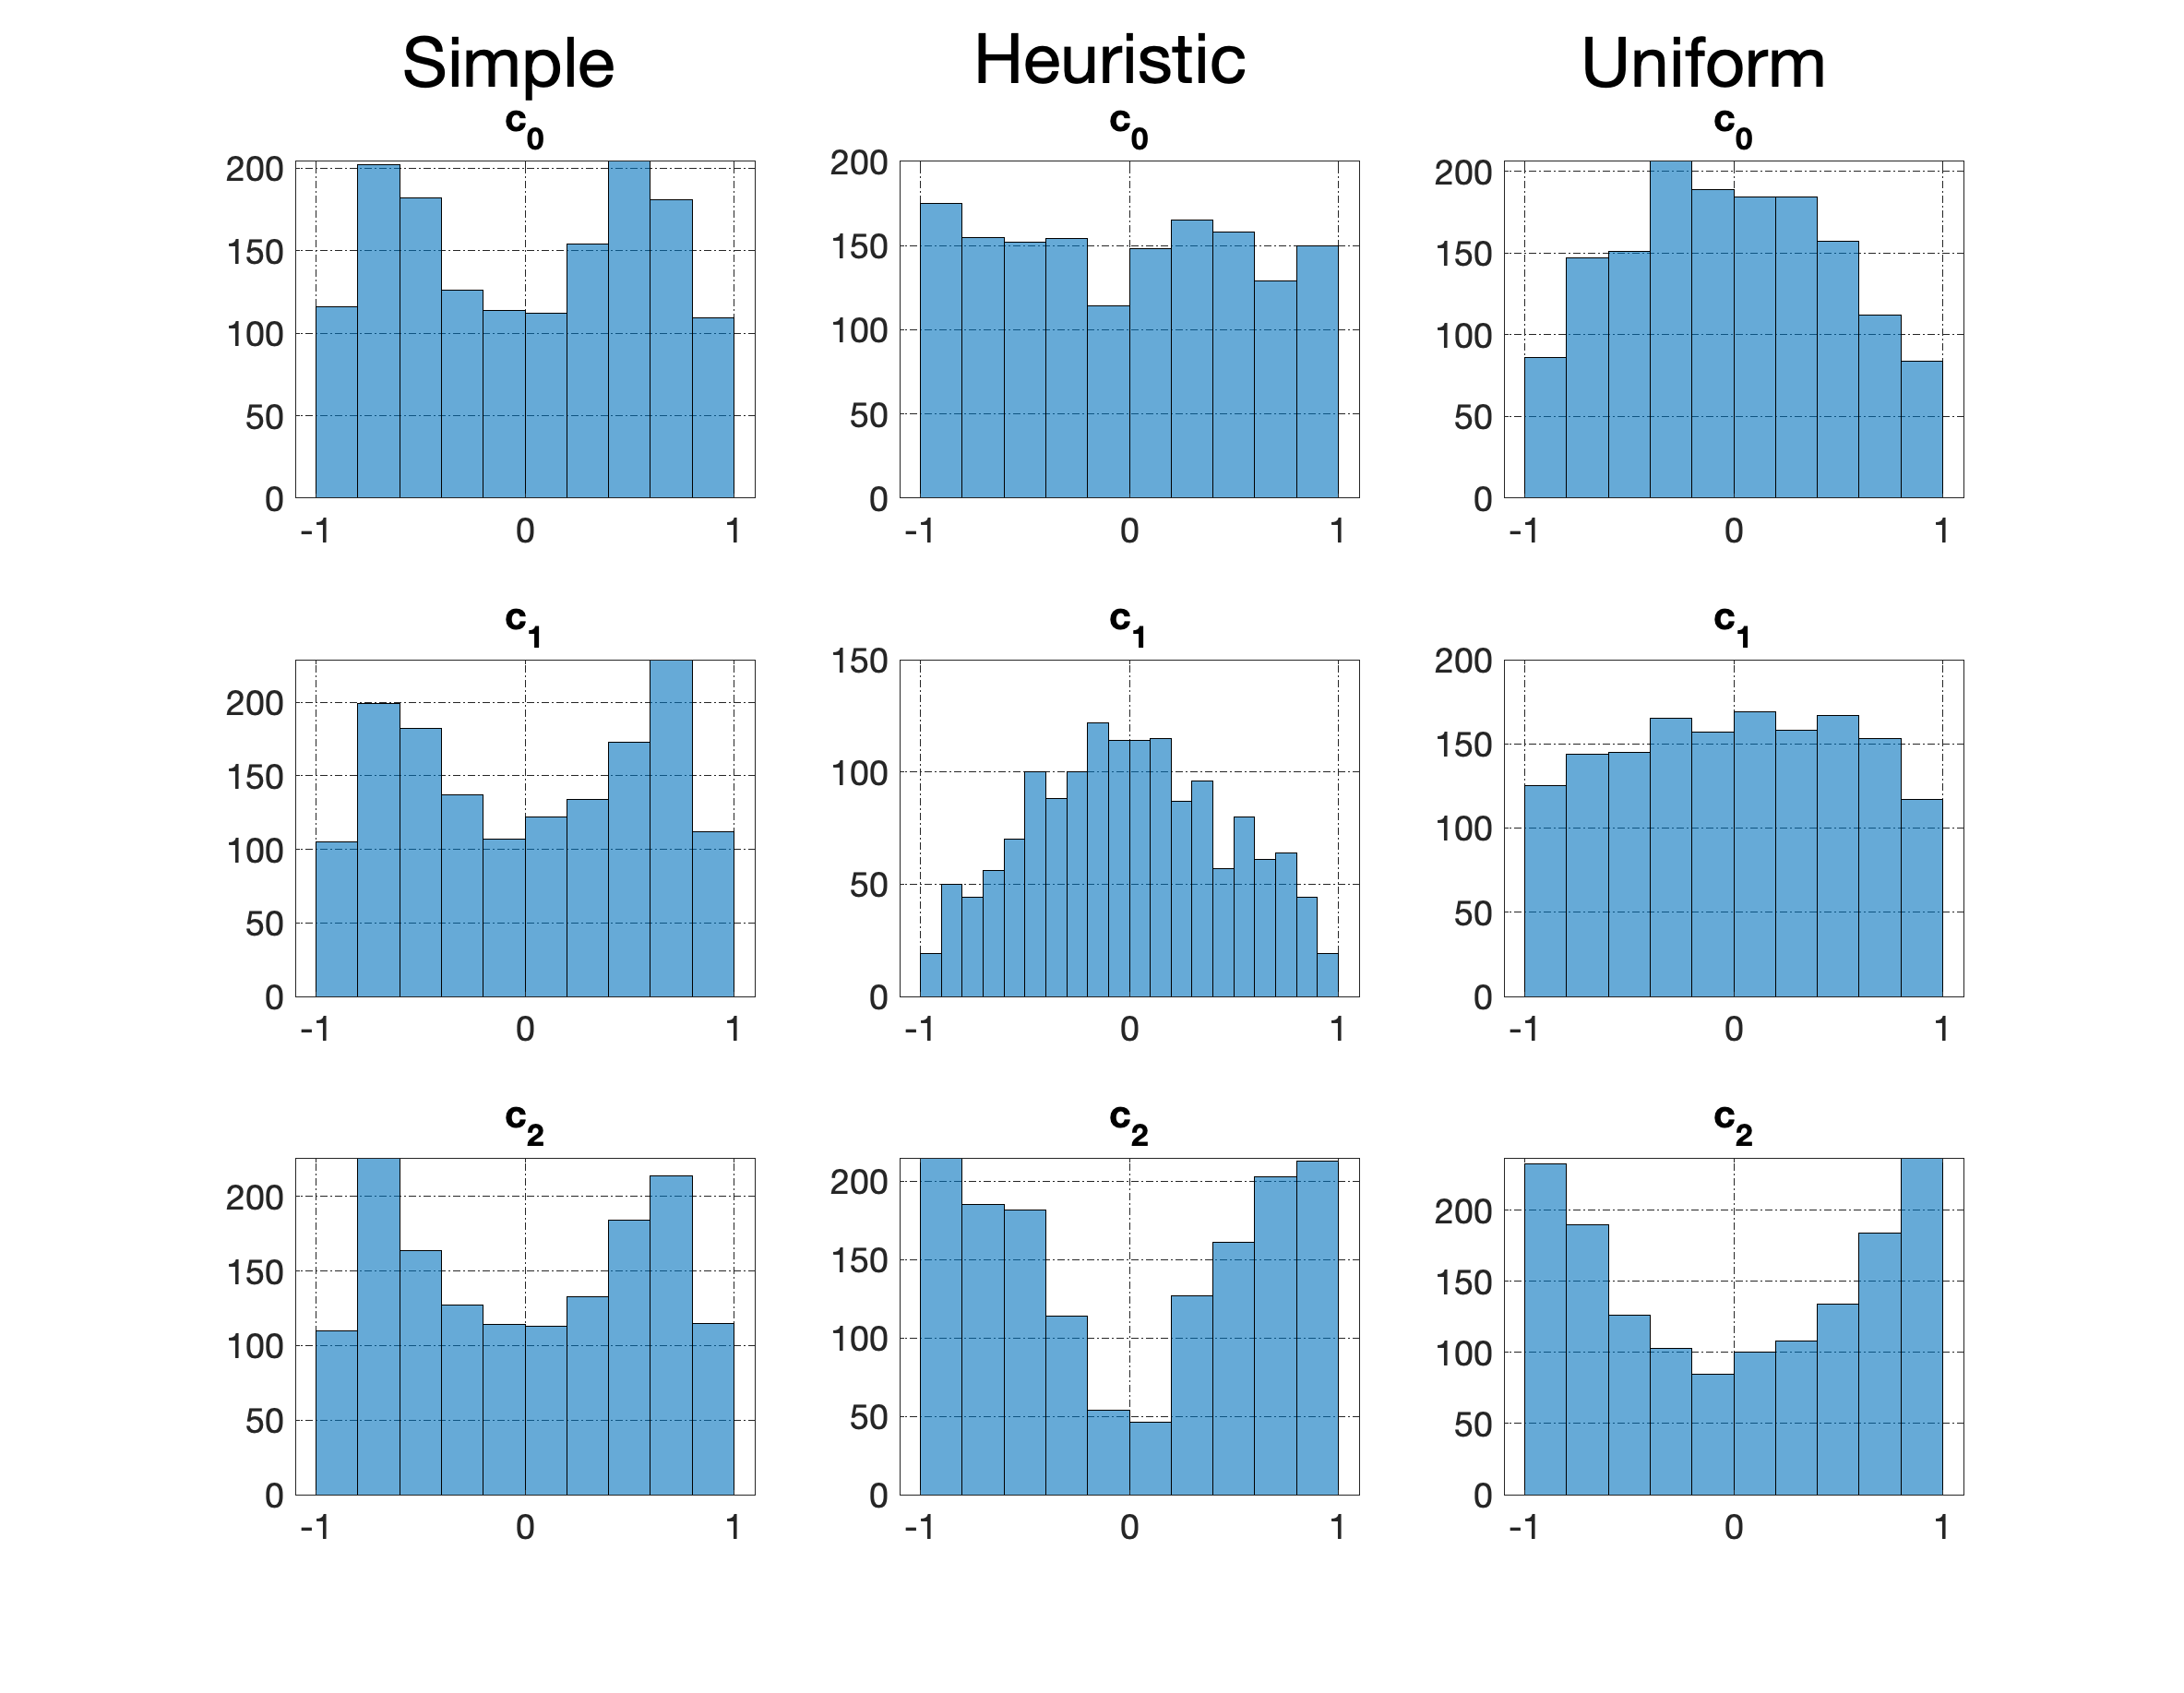
\includegraphics[width=0.7\textwidth]{images/three_coefficients_distribution.eps}
 	\caption{Распределение коэффициентов $C_i$.}
 	\label{fig:ap:three_coefficients_distribution}
 \end{figure}
 
 Пусть $l\in \mathbb{R}^{n}$ --- одна из точек, равномерно распределенных по эллипсу $\{x: x^{\top} (M M^{\top})^{-1} x \leqslant \mu \}$.
 Тогда $\widetilde{C} = M^{\top} (M M^{\top})^{-1} l + z$, где $z \in \operatorname{null}(M)$.
 
 На рисунке \ref{fig:ap:three_coefficients_distribution} приведены гистограммы распределений коэффициентов $C_i$, полученных при помощи описанных двух методов, а также восстановленных из действительно равномерно распределенных по множеству достижимости точек. 
 Видно, что форма распределения коэффициентов в третьей колонке ближе к распределениям во второй колонке, чем к первой. 
 
 \subsection{Особенность линейных управлений}
 \begin{figure}[ht!]
 \centering
 	\hspace{-2.5ex}
 	\begin{minipage}[b]{.4\linewidth} 
 		\small
 		\centering 
 		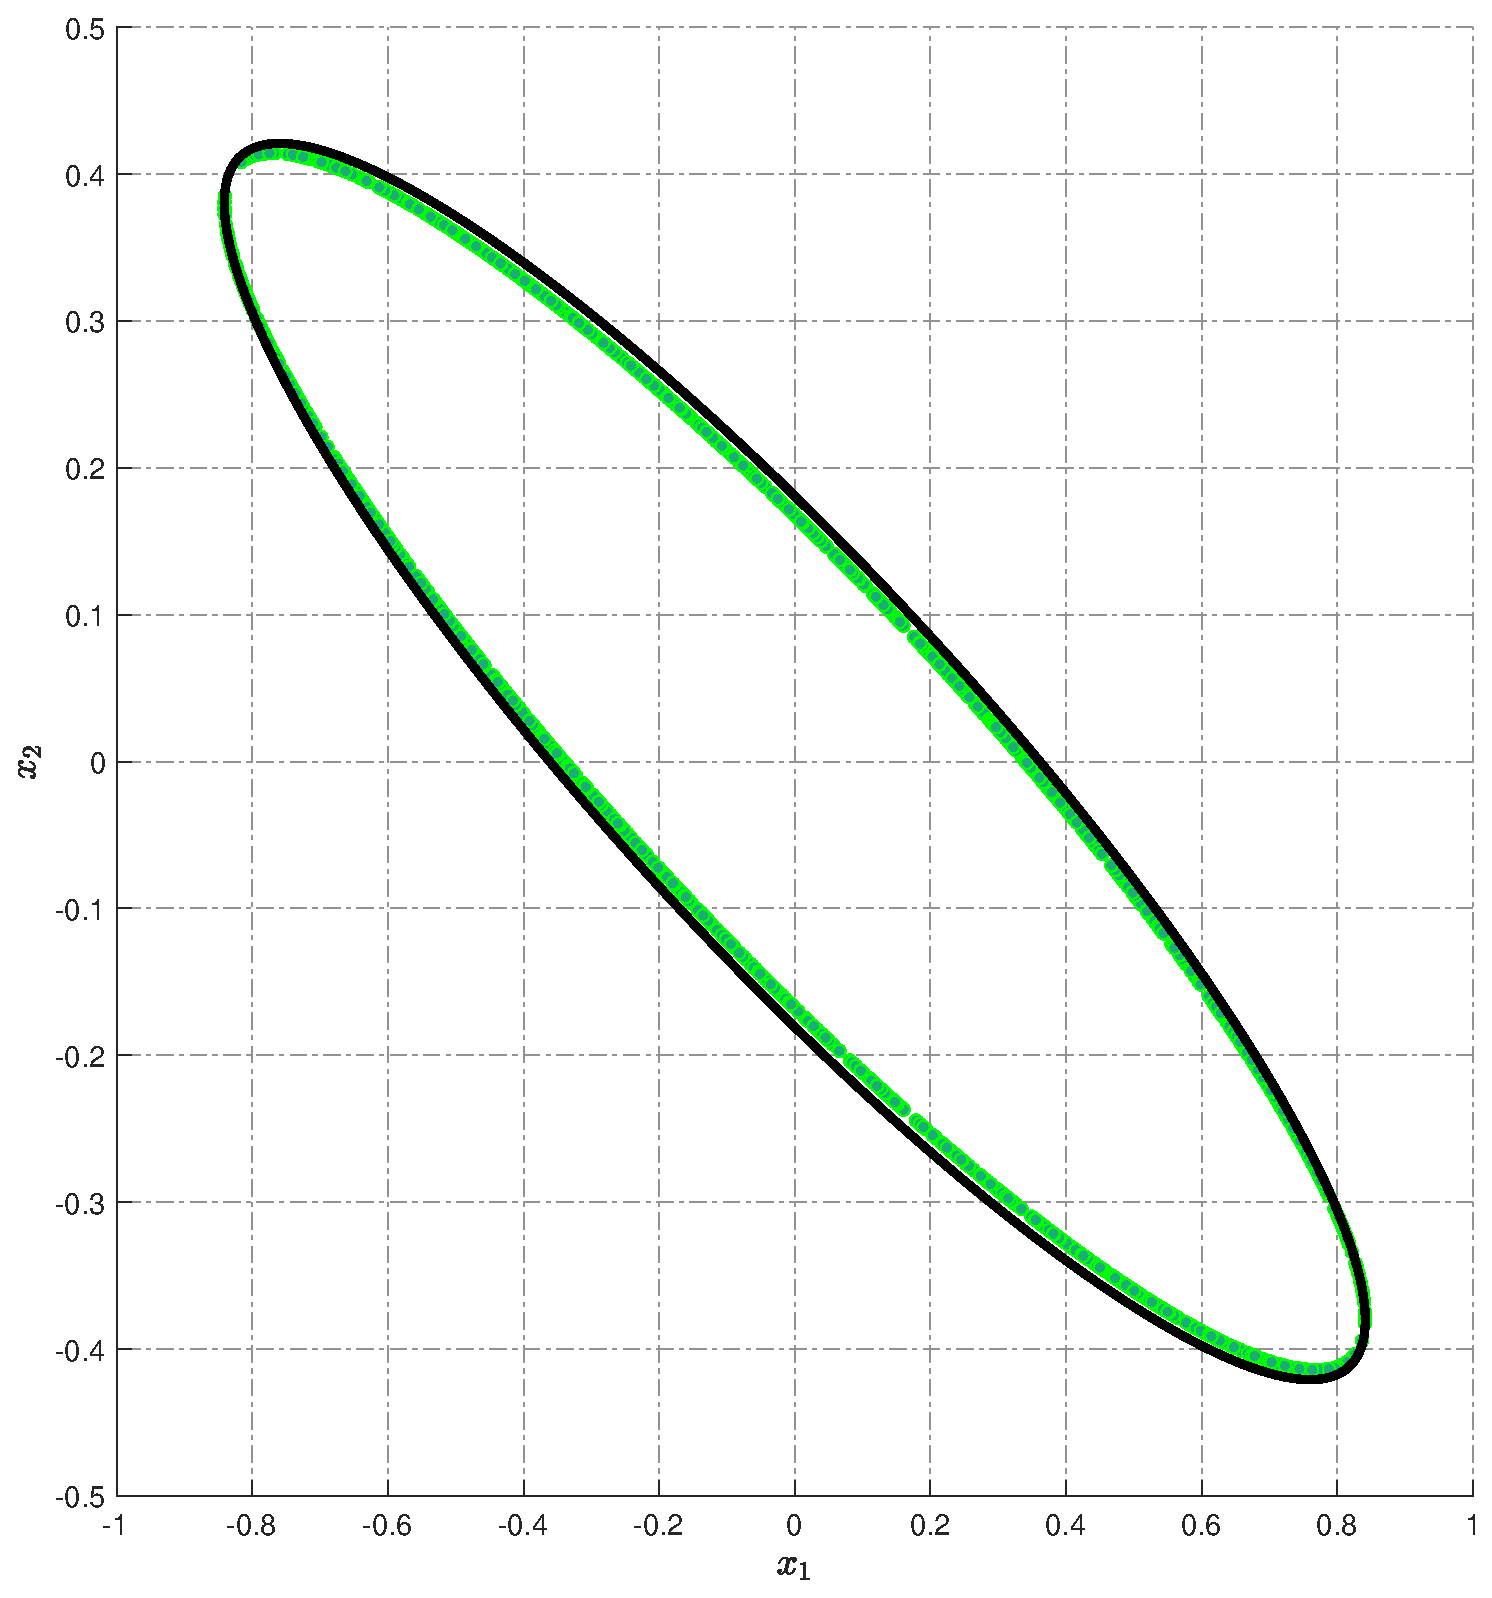
\includegraphics[width=\linewidth]{images/linear_system_linear_control.eps}
 		\subcaption{$ N = 10^3 $ } 
 		 \label{fig:ap:random_linear_system}
 	\end{minipage}
 	\hfill
 	\begin{minipage}[b]{.4\linewidth} 
 		\small
 		\centering
 		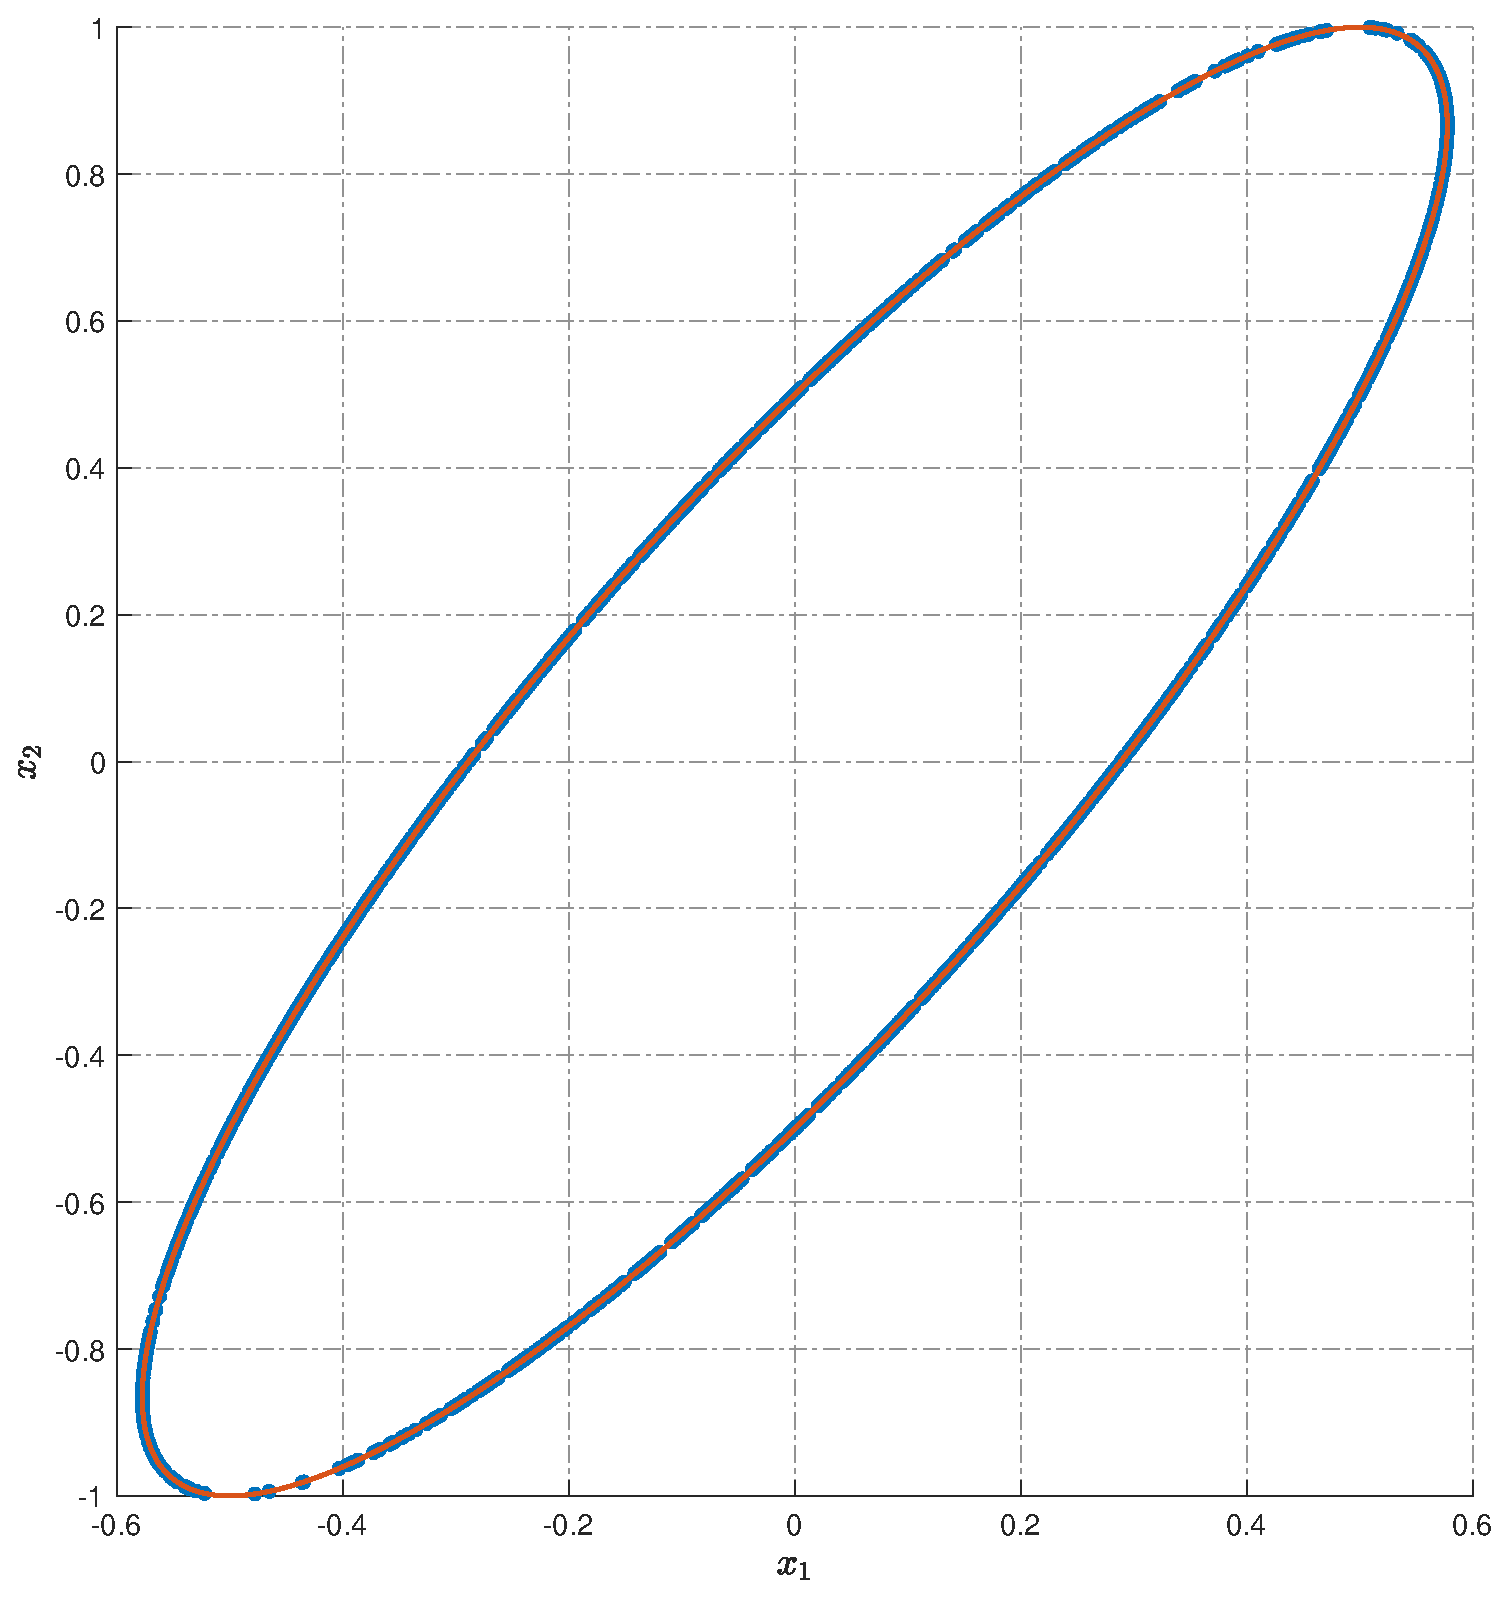
\includegraphics[width=\linewidth]{images/double_integrator_linear_control.eps}
 		\subcaption{$ N = 10^4 $ }
 		 \label{fig:ap:double_intrgrator} 
 	\end{minipage} 
 	\caption{Использование линейных управлений для линейных систем.}\label{fig:ap:linear_control}
 \end{figure}
 
 Другой особенностью, замеченной при изучении Алгоритма \ref{ap:method} является интересный эффект при использовании полиномов 1-ого порядка, то есть линейных по времени управлений, для построения множеств достижимости линейных систем.
 Точки, порождаемые такими управлениями, лежат на эллипсе, который может быть близок к границе истинного множества достижимости (Рис. \ref{fig:ap:random_linear_system}), а иногда и совпадать с границей (Рис. \ref{fig:ap:double_intrgrator}). 
 
 На рисунке \ref{fig:ap:random_linear_system} показано множество достижимости линейной системы
 \begin{gather}\label{ap:random_linear_system}
 	\begin{pmatrix} 
 		\dot{x}_1 \\
 		\dot{x}_2 
 	\end{pmatrix} = 
 	\begin{pmatrix}
 		0 & 1 \\
 		-2 & -3
 	\end{pmatrix}
 	\begin{pmatrix} 
 		x_1 \\
 		x_2 
 	\end{pmatrix} +
 	\begin{pmatrix} 1 \\ 0
 	\end{pmatrix} u.
 \end{gather}
 в момент времени $t = 1$, с нулевыми начальными условиями $x_1(0) = x_2(0) = 0 $ и ограничениями на управление 
 \begin{gather*}
 	\int\limits_0^1 u^2dt \leqslant 1.
 \end{gather*}
 Используются полиномы первого порядка, то есть $u_i(t) $ линейно зависят от времени.
 
 На рисунке \ref{fig:ap:double_intrgrator} показано множество достижимости линейной системы
 \begin{gather}\label{ap:double_intrgrator}
 \dot{x}_1 = x_2,\\
 	\dot{x}_2 = u
 \end{gather}
 в момент времени $t = 1$, с такими нулевыми начальными условиями $x_1(0) = x_2(0) = 0 $ и такими же ограничениями на управление 
 \begin{gather*}
 	\int\limits_0^1 u^2dt \leqslant 1.
 \end{gather*}
 Как и в соседнем примере, используются полиномы первого порядка, то есть $u_i(t) $ линейно зависят от времени.
 
 Для того, чтобы понять причину этого эффекта, рассмотрим задачу оптимального управления
 \begin{gather*}
 	c^{\top} x(1) \rightarrow \max, \\
 	s.t. 	\int\limits_0^1 u^2dt \leqslant 1.
 \end{gather*}
 
 В случае системы \eqref{ap:double_intrgrator} ее решение имеет вид
 \begin{gather*}
 	u(t) = \frac{c_1(1 - t) + c_2}{\sqrt{\frac{c_1^2}{3} + c_1 c_2 + c_2^2}}, \qquad c = \big(c_1, c_2 \big)^{\top}
 \end{gather*}
 
 В случае произвольной системы $\dot{x} =Ax + Bu$ имеем
 \begin{gather}\label{ap:optimal_control}
 	u(t) = \frac{1}{\sqrt{c^{\top}Wc}} B^{\top} \operatorname{exp}\big(-A^{\top}(1-t)\big) c,
 \end{gather}
 где $W$ --- грамиан управляемости, $W = \int\limits_{0}^{1} \operatorname{exp}\big(A(1-\tau)\big) B B^{\top} \operatorname{exp}\big(A^{\top}(1-\tau)\big) d\tau$.
 
 Таким образом, для того, чтобы управление переводило систему \eqref{ap:double_intrgrator}, в граничную точку множества достижимости, необходимо и достаточно, чтобы оно линейно зависело от времени, а также, чтобы норма этого управления в $\mathbb{L}_2[0,1]$ была равна 1. 
 
 В случае линейных двумерных систем, отличных от \eqref{ap:double_intrgrator}, множество точек, в которые система может быть переведена при помощи линейных управлений, является линейным преобразованием окружности.
 Если матрица $M$ этого преобразования, определенная в \eqref{ap:matrix_M}, невырождена, то точки будут лежать на эллипсе. 
 Такие случаи можно видеть на рисунках \ref{fig:ap:linearN104k1T1}, \ref{fig:ap:linearN5105k1T10}, \ref{fig:ap:oscilN5103k1T1}, \ref{fig:ap:oscilN5104k1T1} и \ref{fig:ap:random_linear_system}.
 При малых $T$, оптимальное управление \eqref{ap:optimal_control} может быть достаточно точно приближено линейными функциями. 
 В этом случае, точки будут лежать достаточно близко к границе множества достижимости (Рис. \ref{fig:ap:linearN104k1T1}, \ref{fig:ap:oscilN5103k1T1}, \ref{fig:ap:oscilN5104k1T1} и \ref{fig:ap:random_linear_system}).
 Однако, при увеличении $T$, ошибка аппроксимации оптимального управления линейными функциями будет увеличиваться, что приведет к тому, что точки уже не будут близки к границе (Рис. \ref{fig:ap:linearN5105k1T10}). 
 Если матрица вырождена, то точки будут лежать на отрезке, как на рисунках \ref{fig:ap:oscilN5103k1T2pi}, \ref{fig:ap:oscilN5104k1T2pi}).
 
 \subsection{Другие примеры}
 
 Для построения иллюстраций в диссертации был широко использован Алгоритм \ref{ap:method}, приведем здесь примеры некоторых систем, обладающих наиболее интересными по форме множествами достижимости.
 
 \textbf{Пример 1}. На рисунке \ref{fig:Duffing} показано множество достижимости системы 
 \begin{gather}\label{ap:Duffing}
 	\dot{x_1} = x_2, \qquad
 	\dot{x_2} = -x_1 - 10 \varepsilon x_1^3 + u,
 \end{gather}
 для момента времени $t = 2$, различных значений $\varepsilon$, при нулевых начальных условиях $x_1(0) = x_2(0) = 0 $ и ограничениях на управление 
 \begin{gather}\label{ap:Duffing_controls}
 	\int\limits_0^2u^2dt \leqslant 1.
 \end{gather}
 	 
 	 \textbf{Пример 2}. На рисунке \ref{fig:LinearDubins} показано множество достижимости системы 
 \begin{gather}\label{ap:Linear+Dubins}
 	\begin{pmatrix} 
 		\dot{x}_1 \\
 		\dot{x}_2 \\ 
 		\dot{x}_3 \end{pmatrix} = 
 	\begin{pmatrix}
 		0 & 1 & 0 \\
 		0 & 0 & 1 \\
 		0 & 0 & 0
 	\end{pmatrix}
 	\begin{pmatrix} 
 		x_1 \\
 		x_2 \\ 
 		x_3 \end{pmatrix} + 
 	\varepsilon
 	\begin{pmatrix}
 		\cos x_3 - x_2\\
 		\sin x_3 - x_3 \\
 		0
 	\end{pmatrix} + 
 	\begin{pmatrix}
 		0 \\ 0 \\ 1
 	\end{pmatrix} u.
 \end{gather}
 	для момента времени $t = 1$, различных значений $\varepsilon$, при нулевых начальных условиях $x_1(0) = x_2(0) = x_3(0) = 0 $ и таких же ограничениях на управление, как в предыдущем примере, но на интервале времени $0 \leqslant t \leqslant 1$.
 	
 	\begin{figure}[t]
 		\centering
 			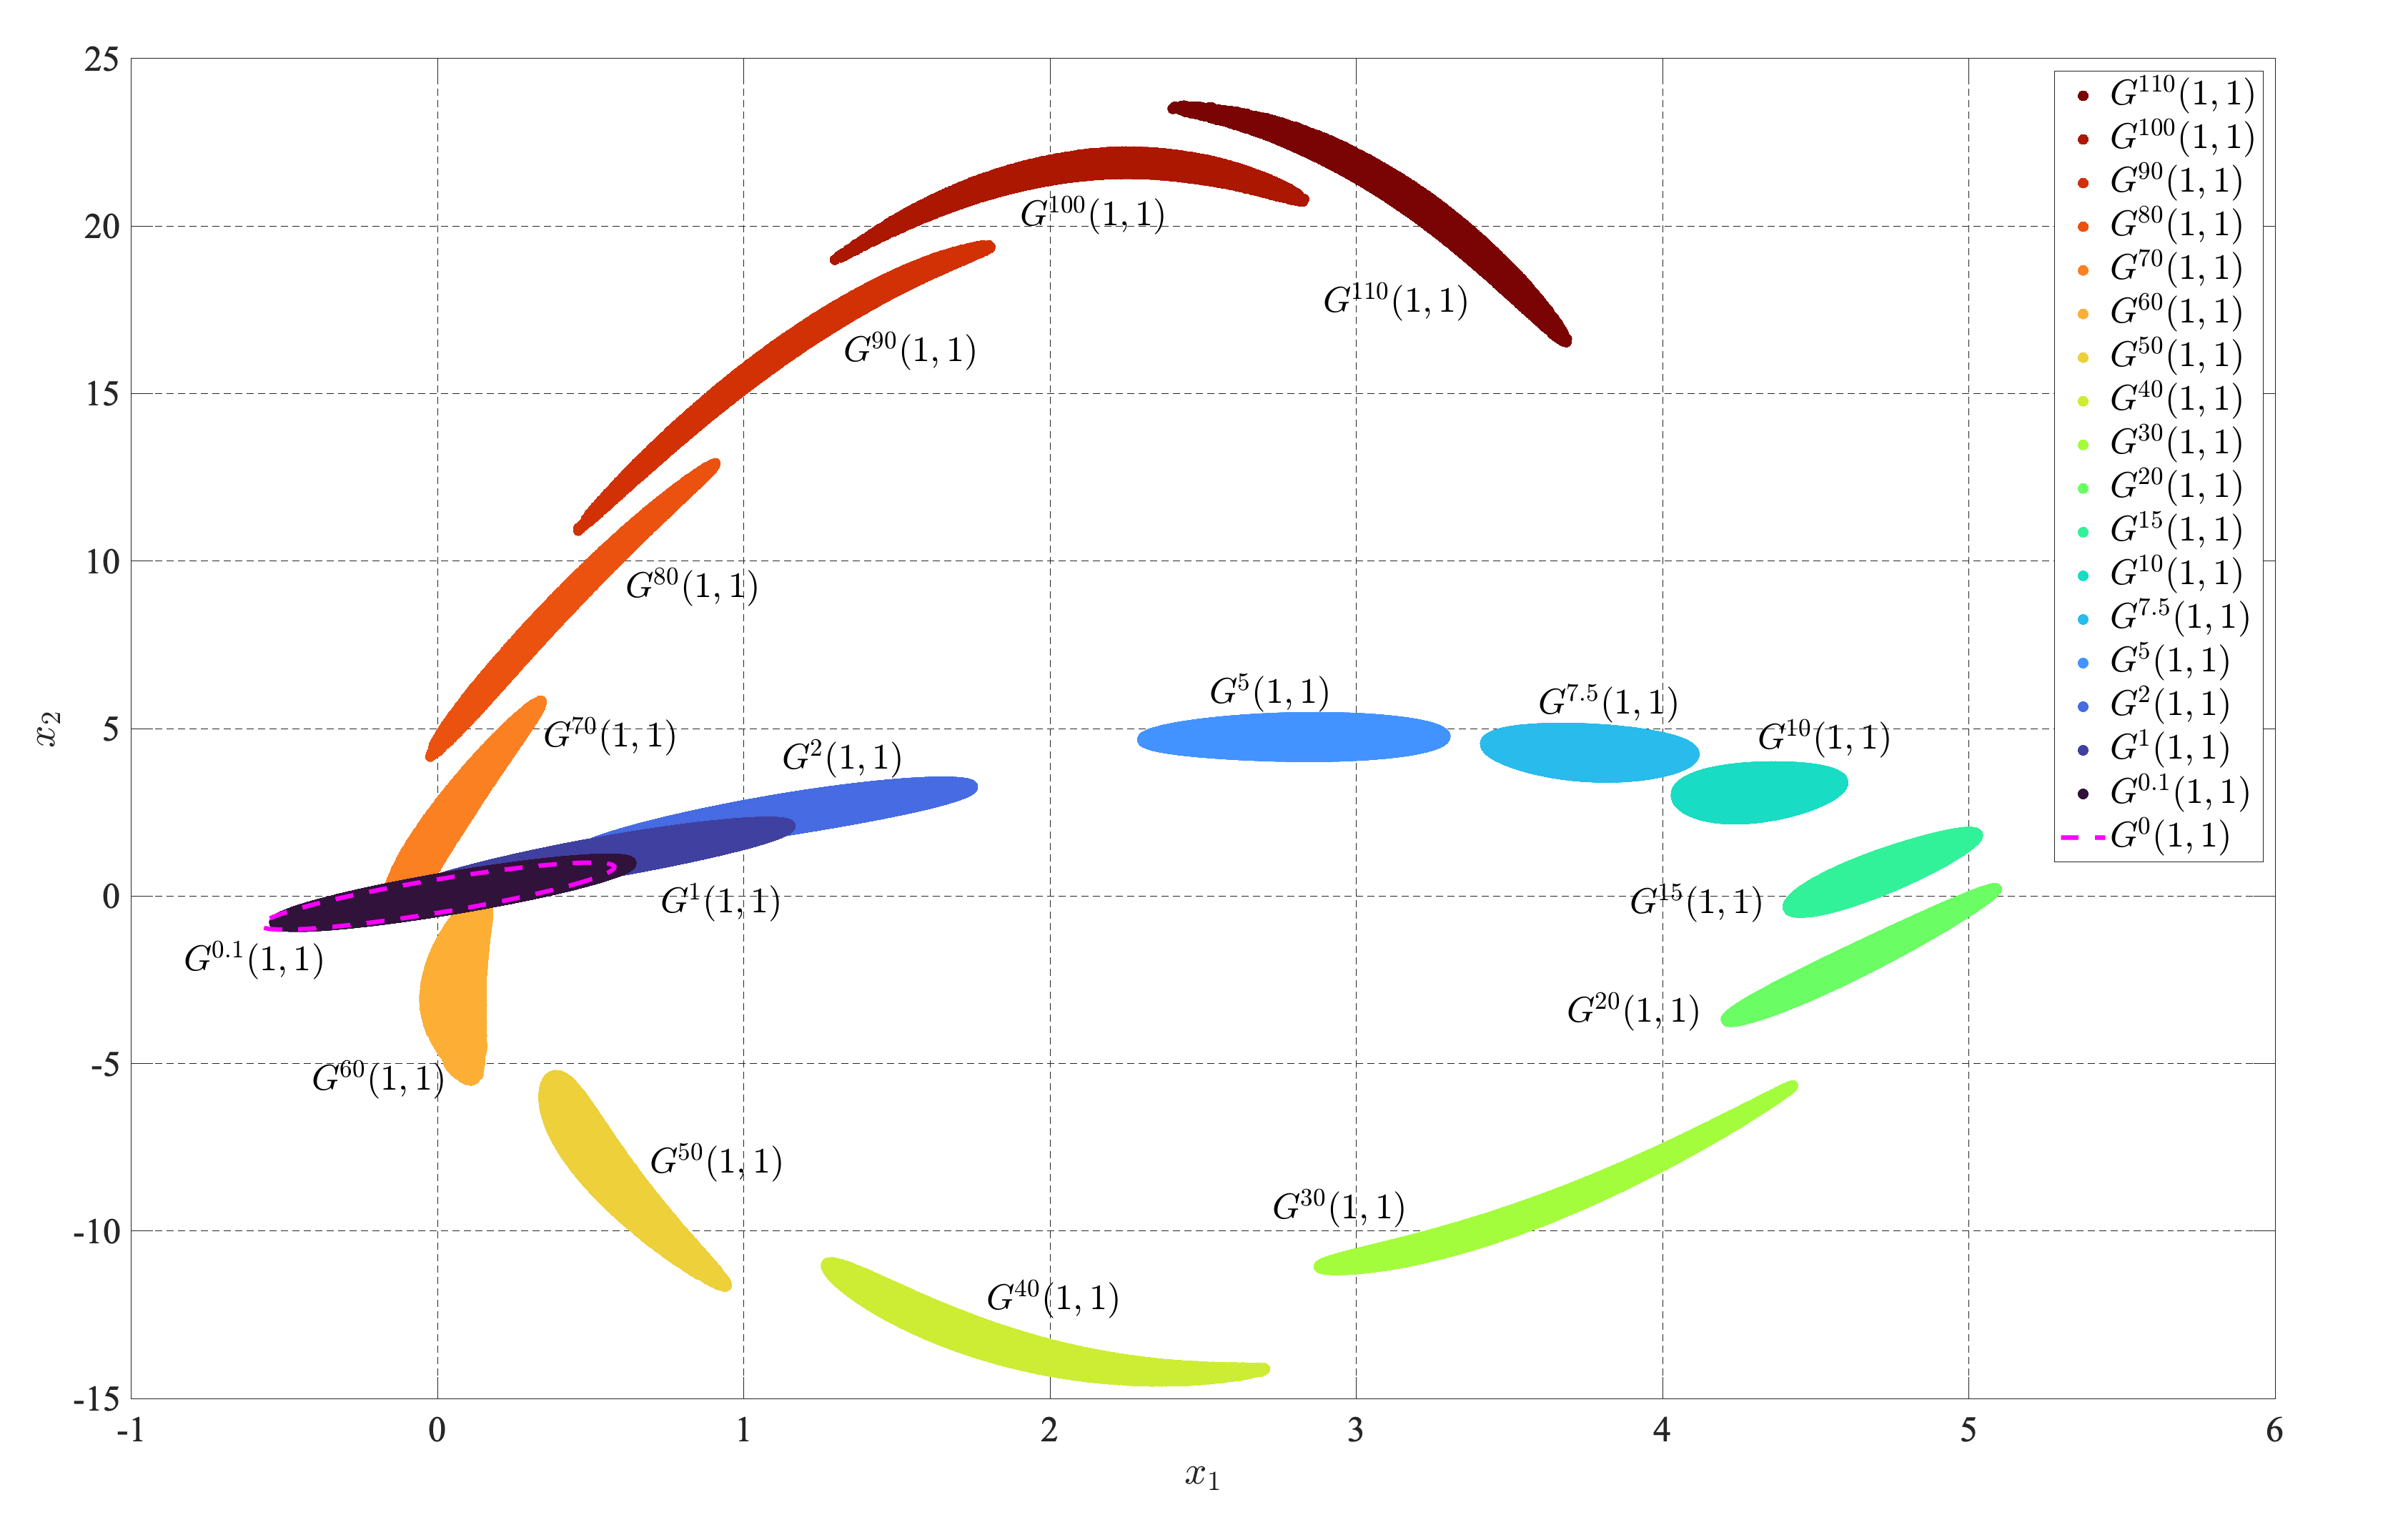
\includegraphics[width=0.92\textwidth]{images/Osipov_QuaziLinearExp.eps}
 		\caption{Множества достижимости системы \eqref{ap:Example3}.}
 		\label{ap:fig:QuaziLinearExp}
 	\end{figure}
 
 \textbf{Пример 3}. На рисунке \ref{ap:fig:QuaziLinearExp} показано множество достижимости системы 
 \begin{gather}\label{ap:Example3}
 	\dot{x_1} = x_2, \qquad
 	\dot{x_2} = u + \varepsilon(\sin x_1 + \cos x_1),\qquad 0\leqslant t \leqslant 1.
 \end{gather}
 Начальное состояние $x_1(0) = x_2(0) = 0 $, управление ограничено 
 \begin{gather}\label{example3_controls}
 	\int\limits_0^1 u^2dt \leqslant 1.
 \end{gather}
 
\end{document}